\renewcommand{\imagepath}{../40-coils/img}

\chapter{Feshbach and Gradient Field Coils}

In this chapter, the design and characterization of the coils used for creating steep magnetic gradients for the 3-dimensional magneto-optical trap and a strong homogeneous magnetic fields for tuning Feshbach resonances is presented. These coils are going to be called \textit{Feshbach coils} in this chapter.

\section{Requirements and Constraints}
In this section, all requirements and constraints in terms of field strength, geometry, stability and field curvature for the coils are elaborated. The next section describes how the coils were specified in order to fulfill these constraints. 
\todo{Would it make more sense to combine these two sections into one?}

\subsection*{Magnetic Field Strength}
The Feshbach coils serve two main purposes in the FermiQP demonstrator. On the one hand, they provide magnetic gradients on the order of \SIrange[]{1e1}{1e2}{\gauss\per\centi\meter}\footnote{Definition of the unit \href[]{https://www.youtube.com/watch?v=_3_JVVs2Kls}{Gauss}: $\SI{1}{\gauss} = \SI{1e-4}{\tesla}$} for the 3-dimensional magneto optical trap. On the other hand, they need to produce homogeneous magnetic fields for scanning over the Feshbach resonance of lithium at \SI{832}{\gauss}. A maximum field of \SI{1300}{\gauss}, created at a current of $I = \SI{400}{\ampere}$, was set as a target for the coil setup.

In order to generate these homogeneous fields, the coils are arranged in Helmholtz configuration, meaning that two equally-sized circular coils are placed on a common axis such that their distance is equal to their radius. The effective ratio of distance and radius required for homogeneous fields, however, depends on the finite size of the coils.

\subsection*{Geometry}
In order to produce the high Feshbach fields in the glass cell with reasonable currents, the radius of the coils should be kept as small as possible, and they should be placed as close to the glass cell as possible.

The coils will enclose the two objectives sitting above and below the glass cell between them. This introduces a minimum distance of around \SI{50}{\milli\meter} between the coils still allowing a few \si[]{\milli\meter} of leeway to fit the objectives between the coils. It was decided for a distance of \SI{55}{\milli\meter} between the innermost wires of the coils, not considering additional surface material on the coils. These geometrical constraints allow an estimation of the number of windings needed to attain the required \SI{1300}{\gauss} of field in Helmholtz configuration to 30, which was determined using simulations (see sections~\ref{ch:simulation} and~\ref{ch:coil_properties}).

The orientation of the coil arrangement is constraint by the requirement to drive Raman transitions on the atoms in the optical lattice with $\pi$-polarized light shone in through the objectives. $\pi$ transitions can only be driven with light having a polarization parallel to the quantization axis of the atoms, which is set by the direction of the magnetic field. Light shone in along the $z$ axis through the objectives can only be $\pi$-polarized in the $xy$ plane, constraining the direction of the magnetic field to the $xy$ plane. It was decided to align the coil arrangement axis with the $y$ axis of the experiment chamber, meaning that the two coils sit on the left and on the right of the glass cell with the coil axis passing through the trap region of the magneto-optical trap.

Figure~\ref{fig:feshbach_coil_geometry_constraints} shows the geometrical constraints on the position of the coils.

\begin{figure}
    \centering
    \includegraphics[]{\imagepath/feshbach_coil_geometry_constraints/feshbach_coil_geometry_constraints.pdf}
    \caption{Position of the Feshbach coils with respect to the glass cell and the objectives: The objectives (\SI{44}{\milli\meter} diameter) which are positioned below and above the glass cell are enclosed by the two coils, setting the minimum distance between the coils. The innermost coil wires have a distance of \SI{55}{\milli\meter}.}
    \label{fig:feshbach_coil_geometry_constraints}
\end{figure}

As the coils have many windings, thus having a significant size, and are close to the glass cell, they block a significant part of the optical access to the location of the atoms. Many laser beams and imaging signals must, however, be shot into and received from the glass cell, demanding that the coils leave open as much optical access to the glass cell as possible. Most notably, the beams of the magneto-optical trap need to enter the glass cell on the $y$ axis through the left and right surfaces, the pinning lattice beams also enter there with incidence angles of $\pm \SI{45}{\degree}$. On the short side of the glass cell, the science lattice beams enter with incidence angles of around $\pm \SI{15}{\degree}$. The available space for the coils is hence bound by these laser beams. In order to minimize the blocked optical access, a cone-shape coil geometry with parallelogram-shaped cross-section, consisting of $6 \times 5$ windings, was opted for, as depicted in figure~\ref{fig:parallelogram_cross_section}. The opening angle of the cone has been set to $\SI{45}{\degree}$ because then the Helmholtz condition of equal coil distance and radius is approximately fulfilled for every layer.
\begin{figure}
    \centering
    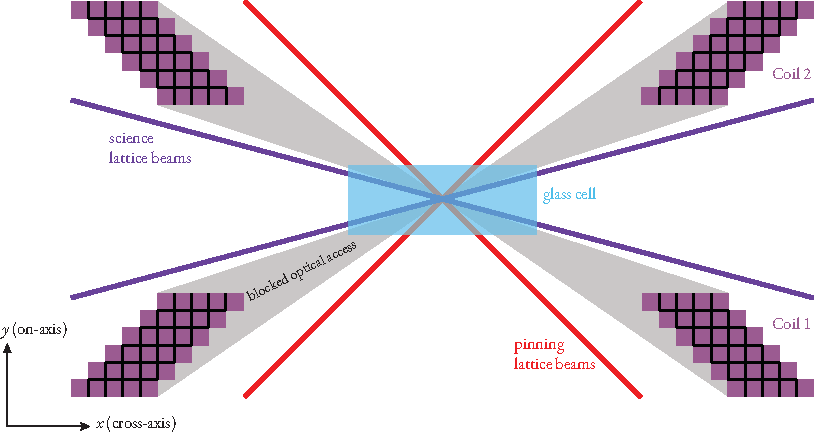
\includegraphics[]{\imagepath/parallelogram_cross_section/parallelogram_cross_section.pdf}
    \caption{Parallelogram-shaped cross-section of the coils for minimizing the blocked optical access into the glass cell, letting the pinning and science lattice beams pass alongside the coil (view from above): The windings layers stacked onto each other (in the coil axis direction) have radii that increase by one wire size per layer (cross-axis direction).}
    \label{fig:parallelogram_cross_section}
\end{figure}

\subsection*{Field and Temperature Stability}
The FermiQP demonstrator aims for a relative field stability of \SI{e-7}{} calling for an active stabilization mechanism. For this purpose, both coils are independently driven by two independent power supplies enabling fast switching.

Furthermore, it is important to ensure thermal stability of the coils. The electrical power $P(I) = RI^2$ dissipated in the coils with resistance $R$ shows quadratic scaling  with the driving current $I$. For an exemplary coil with \SI{10}{\milli\ohm} resistance driven with $I = \SI{400}{\ampere}$ this would amount to a dissipated power of \SI{1.6}{\kilo\watt} converted into heat. In order to transport this heat off efficiently, avoiding a critical increase of temperature, the coil must be made of hollow-core wires allowing for water-cooling. For a given maximal temperature increase $\Delta T$ of the cooling water, the cooling power of the water can be estimated as
\begin{align}
    Q_\text{cool} = c_\text{water} ~ \Delta T ~ m_\text{water} ~ v_\text{flow}
\end{align}
with the heat capacity $ c_\text{water}$ of water, the specific mass $m_\text{water}$, and the speed $v_\text{flow}$ of the cooling water flow, which depends on the applied pressure, the turbulence of the flow, and the wire geometry.

To lower the required cooling water pressure and to avoid turbulences in the cooling water stream, it was decided to separate the wire layers of the coils into pancakes of two layers each constituting separately driven water cooling circuits, as shown in figure~\ref{fig:pancake_structure}. For this the two supply lines for each pancake are placed next to each other, forming pairs of wires with current flowing in opposite directions. This has the additional advantage that the fields of the supply lines cancel out in the far-field and do not influence the magnetic field in the center of the coil arrangement.

\begin{figure}
    \centering
    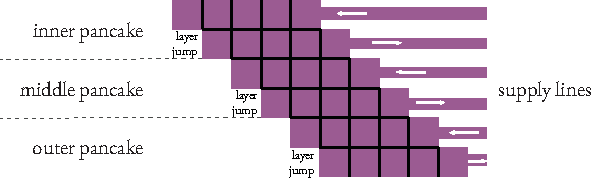
\includegraphics[]{\imagepath/pancake_structure/pancake_structure.pdf}
    \caption{Cross-section of the pancake structure of the coils: Two layers of wire are combined into a so-called pancake that constitutes a single water cooling circuit. The layers have layer jump on the innermost winding where the wire hops from one layer to the other. The current in the two supply lines for each pancake is flowing in opposite directions such that the magnetic fields originating from the wire cancel out in the far-field.}
    \label{fig:pancake_structure}
\end{figure}

\subsection*{Field Curvature}\label{ch:field_curvature_definition}
When the atoms trapped in the optical lattice are exposed to the homogeneous Feshbach field, they experience an energy shift resulting from the interaction of the magnetic moment $\vec \mu$ with the field that can lead to trapping or anti-trapping effects $\vec B$~\cite{pritchard_cooling_1983,gehm_properties_2003, hagemann_setup_2020}:
\begin{align}
    E_{B, {\text{high-field seeker} \atop \text{low-field seeker}}} = \mp \vec \mu \vec B
\end{align}
where the sign of the shift depends on whether the atoms are in high- or low-field seeking states. The magnitude of the magnetic moment is $\mu \approx \mu_\text{B}$ with the Bohr magneton $\mu_\text{B} = \SI{9.27e-24}{\joule\per\tesla}$.

In the very center of the coil arrangement, the magnetic field in the Helmholtz operation mode of the coils is completely homogeneous. Realistically, however, there is a non-negligible position dependence $B(\vec r)$ of the field, stemming from the finite size of the region of interest and imperfections in positioning, aligning, and manufacturing of the coils. This leads to a position-dependent potential that the atoms are exposed to:
\begin{align}
    \hat H(\vec r) = \frac{\vec p^2}{2m} \mp \vec \mu \vec B(\vec r)
\end{align}

Assuming that the magnetic field around the center of the coil arrangement follows a paraboloid shape, in one dimension $B(q) = B_0 + a_q q^2$ with a field curvature coefficient $a$ and a spatial coordinate $q$, one can identify the magnetic potential with a quantum mechanical harmonic oscillator:
\begin{align}
    \underbrace{V_0 + \frac{1}{2}m\omega^2q^2}_{V_\text{HO}(q)} ~~~\equiv~~~ \underbrace{\mp \mu B(q) = \mp \mu B_0 \mp \mu a_q q^2}_{V_\text{magnetic}(q)}
\end{align}

Identifying the position-dependent terms, the magnetic potential can be assigned the angular trap frequency $\omega_{\vec q}$ along the $\vec q$ coordinate axis:
\begin{align}\label{eq:trap_omega_definition}
    \omega_{\vec q} = \sqrt[]{\mp\frac{2 \mu a_{\vec q}}{m}} = \sqrt[]{\mp\frac{2 \mu_\text{B} a_{\vec q}}{m}}
\end{align}
In the following, the trapping potential is considered trapping in the ${\vec q}$ direction if $\omega_{\vec q}$ is real, and anti-trapping if $\omega_{\vec q}$ is imaginary. For high-field seekers, the potential is trapping if $a_{\vec q} < 0$ and anti-trapping if $a_{\vec q} > 0$. For low-field seekers, the potential is trapping if $a_{\vec q} > 0$, and anti-trapping if $a_{\vec q} < 0$. This can be intuitively seen as high-field seekers are trapped if the field is concave and has a maximum, hence $a_{\vec q} < 0$, and the other way around for high-field seekers. Plots of exemplary trapping and anti-trapping field landscapes are shown in figure~\ref{fig:magnetic_field_curvature_examples}.

In a two-coil field, if the potential is trapping along the arrangement axis, it is anti-trapping in the cross-axis directions, and vice versa. This is due to Earnshaw's theorem~\cite{earnshaw_nature_1842} stating that a magnetic field in three dimensions has the shape of a hyperboloid, and thus cannot have a global extremum rather than a saddle point, implying that the magnetic field is curved into opposite directions on two axes. The field in the coil-axis direction is curved twice as much as in the cross-axis direction: $\frac{a_\text{on-axis}}{a_\text{cross-axis}} = -2$, hence the trap frequencies have a ratio of $\frac{|\omega_\text{on-axis}|}{|\omega_\text{cross-axis}|} = \sqrt{2}$~\cite{hagemann_setup_2020}.

Note that $a_{\vec q}$ relates to the field landscape along ${\vec q}$ as $a_{\vec q}  = \frac{1}{2} \pdv[2]{B}{q}$ which can be seen from the Taylor expansion $B(q) = \eval{B}_{0} + \eval{\pdv{B}{q}}_{0} q + \frac{1}{2} \eval{\pdv[2]{B}{q}}_{0} q^2 + \mathcal{O}(q^3)$ around $0$ identifying the second order term with $a_{\vec q} q^2$.

\begin{figure}
    \caption{Trapping and anti-trapping field landscapes for high-field seekers: If the curvature $a_q$ is negative, the atoms are trapped in the maximum of the magnetic field.}
    \label{fig:magnetic_field_curvature_examples}
\end{figure}

The design goal for the coil arrangement with regard to the field curvature is to minimize the absolute trap frequency in each direction by setting the coil distance accordingly.

\section{Simulation}\label{ch:simulation}
In order to determine the optimal specifications and to characterize the coils, a simulation python library was developed (called \textit{coil simulation library} from now on). It makes heavy use of the magnetic field library \textit{magpylib}~\cite{ortner_magpylib_2020, noauthor_magpylibmagpylib_2022} providing magnetic field vectors at arbitrary positions originating from wire loops, straight wires and permanent magnets of different shapes.

\subsection*{Modelling}
The \textit{coil simulation library} models arrangements of two or more coils sharing a common axis. The models are parameterized by the distance $d_\text{coil}$ of the coils to the center, the number $n_\text{coil}$, the radius $r_\text{coil}$, and the arrangement geometry of the windings of each coil, the spacing $w$ between the windings, the geometry of the wire, presence and length of supply lines, and the current $I_\text{coil}$ flowing in each coil and even in each winding if desired.

A coil is modelled as a set $\mathcal{L}$ of circular wire loops $L(r, y, I)$ with radius $r_i$, a center $y$ position $y$, and current $I$. As is the case for the FermiQP demonstrator, the wire loops' axes are parallel to the $y$ axis. For the $n_\text{on-axis} = 6$ on-axis windings and the $n_\text{cross-axis} = 5$ cross-axis windings, each loop $L_{ac}$ with on-axis index $a \in \{0, \ldots, n_\text{on-axis} - 1\}$ and cross-axis index $c \in \{0, \ldots n_\text{cross-axis} - 1\}$ is defined as
\begin{align}
    L_{ac} = L \left(r_\text{coil} + r_{ac}, y_\text{coil} + y_{ac}, I_\text{coil}\right)
\end{align}
with the on-axis ($y$) and radial (cross-axis) offsets
\begin{align}
    y_{ac} &= w\cdot \left(a-\frac{n_\text{on-axis}}{2} + \frac{1}{2}\right) \\
    r_{ac} &= y_{ac} \tan \eta + w \cdot \left(c - \frac{n_\text{cross-axis}}{2} + \frac{1}{2}\right)
\end{align}
where $w$ is the side length of a wire, and $\eta$ is the opening angle of the parallelogram-shaped cross-section of the coil cone ($\eta = \SI{45}{\degree}$ for the coils in the FermiQP demonstrator). Figure~\ref{fig:coil_model} visualizes how a coil is modelled as a set of wires.

This way of modelling a coil neglects the spiral shape of the coil wire as well as the jump between different on-axis layers of the coil.

\begin{figure}
    \caption{Modelling a coil as a set of wires:
    \todo[inline]{add figure}
    }
    \label{fig:coil_model}
\end{figure}

For an arrangement, the library provides the user with sketches of the arrangement, magnetic field vectors and magnitudes at arbitrary positions, plots of fields along trajectories through the arrangement, maps of the field landscape in planes in the arrangement, information about gradients and curvatures of the fields, resistances, inductances, dipole moments, $L\over R$ time constants, and mutually exerted mechanical forces of the coils.

The technical details of the implementation of the \textit{coil simulation library} are outlined in appendix chapter~\ref{ch:coil_simulation_library}. The following paragraphs explain how important characteristics of the coils and fields are calculated in the \textit{coil simulation library}.

\subsection*{Coil properties}
The \textit{coil simulation library} provides the following fundamental coil properties:
\paragraph{Resistance}
The resistance $R$ of a coil is determined using the specific resistance of copper of $\rho_\text{copper} = \SI{1.72e-8}{\ohm\meter}$:
\begin{align}\label{eq:resistance_simulation}
    R_\mathcal{L} = \frac{\rho_\text{copper} \sum\limits_{L \in \mathcal{L}} 2\pi r_L} {w^2 - A_\text{hollow}}
\end{align}
with the cross-section area $A_\text{hollow}$ of the hollow wire.

\paragraph{Inductance and L/R time} The inductance of a coil can be determined as $L = \frac{\Phi}{I}$ with the magnetic flux $\Phi = \int B \dd A$ at a current $I$~\cite{demtroder_zeitlich_2013}. In the \textit{coil simulation library}, the flux through a wire loop $L$ is approximated as $\Phi_L \approx B \cdot \pi r_L^2$ with the total magnetic field $B$. The total inductance of coil $L$ is calculated as
\begin{align}\label{eq:inductance_simulation}
    L_\mathcal{L} = \sum\limits_{L \in \mathcal{L}} \frac{B(y = y_L) \pi r_L^2}{I_L}
\end{align}

For calculating the self-inductance, $B$ was set to the field solely generated by the respective coil. For estimating the inductance of the coil when part of an arrangement of coils, $B$ was set to the field of the whole arrangement. This leads to higher inductances when operated in Helmholtz configuration and lower inductances when operated in gradient configuration. This in-arrangement inductances are only meaningful if the amount of current flowing in all coils is the same and coupled, and if the coils have the same geometry.\footnote{With coupled currents in the individual coils, the whole arrangement can be thought of as a single coil consisting of multiple sub-coils at different positions. The self-inductance of the arrangement is then calculated with the total magnetic field produced by all sub-coils of the arrangement, and can be though of as a sum of the individual inductances of the sub-coils.}\todo{add factor , see Demtroder 2 ch 4.3.2.2}

The time constant $\tau = \frac{L}{R}$ quantifies how fast the current in a coil with inductance $L$ and resistance $R$ can be switched by a sudden change of the applied voltage: $\Delta I(t) \propto 1-\exp \left(-\frac{t}{\tau}\right)$~\cite{demtroder_zeitlich_2013}. In the \textit{coil simulation library}, this time constant is estimated as
\begin{align}\label{eq:time_constant_simulation}
    \tau_\mathcal{L} = \frac{L_\mathcal{L}}{R_\mathcal{L}}.
\end{align}
Using the inductance of the whole arrangement in Helmholtz configuration for $L$ increases  the estimated $\tau$, as the inductance of the whole arrangement of coils with coupled currents is higher and hence has a longer switching time. For the arrangement in gradient mode, the estimated $\tau$ is decreased as the coils' mutual inductance effects have opposite sign.\todo{Verify, does the L modelling and the conclusions for $\tau$ make sense?}

\paragraph{Dipole moment}
The magnetic dipole moment $\vec m$ of a coil determines the force $\vec F = \vec m (\vec \nabla \vec B)$ and torque $T = \vec m \times \vec B$ it experiences in a magnetic field. Furthermore, the magnetic field generated on the coil axis ($y$) by a magnetic moment $\vec m$ amounts to $\vec B = \frac{\mu_0 \vec m}{2\pi y^3}$ in the far-field ($y \gg r$). For a wire loop, it is defined as $\vec m = I \vec A$ with the coil axis vector $\vec A$ having the length of the wire loop cross-section area~\cite{demtroder_statische_2013}. In the \textit{coil simulation library}, the magnetic moment of a coil arrangement $\mathcal{A}$ is calculated as
\begin{align}\label{eq:dipole_moment_simulation}
    m_\mathcal{A} = \sum\limits_{L \in \mathcal{A}} I_L \cdot \pi r_L^2.
\end{align}

\subsection*{Field properties}
The \textit{coil simulation library} provides the following properties of the field generated by an arrangement:

\paragraph{Curvature and Trap Frequency}
The field curvature $a_q$ along an axis $q$ in an arrangement $\mathcal{A}$, as defined in chapter~\ref{ch:field_curvature_definition}, is calculated from sampled magnetic field strength values $B_i(\vec 0 + d \cdot \vec q)$ for distances $d$ from the center along the $\vec q$ axis. In the \textit{coil simulation library}, the curvature is determined in a region of $\SI{+-2}{\milli\meter}$ around the center in \SI{200}{} steps as a default. A degree-7 polynomial $\hat B(d) = \sum\limits_{i=0}^7 c_i d^i$ is fit to the sampled data. The curvature is then the second coefficient of the fit: $a_{\vec q} = \hat c_2$.

The high-field seeker trap frequency is then calculated as (cf. equation \ref{eq:trap_omega_definition})
\begin{align}\label{eq:trap_frequency_simulation}
    f_{\mathcal{A},~\vec q,~\text{high-field seeker}} = \frac{1}{2\pi}  \sqrt{\left| \frac{2 \hat c_2 \mu_\text{B}}{m_{^6\text{Li}}} \right|} (-\mathrm{sgn} \hat c_2)
\end{align}
which is positive if the field is trapping and negative if anti-trapping for high-field seekers along $\vec q$.

\paragraph{Gradient}
The gradient in an arrangement $\mathcal{A}$, meaning the linear components of the field landscape, along $\vec q$ is determined from the same polynomial fit as for the curvature.
\begin{align}\label{eq:gradient_simulation}
    g_{\mathcal{A},~\vec q} = \eval{\pdv[]{B}{q}}_{q = 0} = \hat c_1
\end{align}

\paragraph{Mechanical Force}
The axial mechanical force on a coil $\mathcal{L}$ in the field of an arrangement is estimated using its magnetic moment and the field gradient: $\vec F = \vec m (\vec \nabla \vec B)$. As the magnetic moment only has a $y$ component, only the axial gradient of the field is relevant. For calculating the force on the total coil, its wire loops' magnetic moments $m_L = I_L \cdot \pi r_L^2$ multiplied by the approximated $y$ gradient $\eval{\pdv[]{B}{y}}_{y = y_L} \approx \frac{B(y_L + s) - B(y_L)}{s}$, with a default step length $s = \SI{0.5}{\milli\meter}$, are summed:
\begin{align}\label{eq:mechanical_force_simulation}
    F_\mathcal{L} \approx \sum\limits_{L \in \mathcal L} m_L \cdot \eval{\pdv[]{B}{y}}_{y = y_L} \approx \sum\limits_{L \in \mathcal L} I_L \pi r_L^2 \left(\frac{B(y_L + s)-B(y_L)}{s}\right)
\end{align}

This approximation is coarse, not only because of the approximation of the gradient, but especially because the finite radial extent of the coil was neglected, meaning that the coil was assumed to be small compared to the radial distance on which the $y$ gradient changes.\todo{check validity}




\section{Coil Properties}\label{ch:coil_properties}
In this section, an overview of the geometrical specifications and the operational properties of the Feshbach coils for the FermiQP demonstrator is given. Also, the field generated by a single coil is characterized.


\subsection*{Geometry}
The coils were produced by an external producer (Krämer Energietechnik, Am Escheberger Weg 8a, 34289 Zierenberg, Germany). In consultation with them, the required specifications were determined using the \textit{coil simulation library} optimizing field curvature and peak field in Helmholtz configuration. In total, three coils were purchased, two for operation in the demonstrator and one spare. They are called \textit{Gauss}, \textit{Maxwell}, and \textit{Tesla}.

A center-of-mass radius of \SI{83}{\milli\meter} was decided for. The six layers with five windings each are grouped into three pancakes (outer, middle, and inner). Each pancake has two supply lines that all connect to the coil at the same azimuthal point. All other geometrical specfications as well as some measured geometrical properties on the three coils are listed in table~\ref{tab:coil_geometrical_properties}.

\begin{table}
    \centering
    \begin{tabular}{rcccc}
        \toprule
        & specified & \textit{Gauss} & \textit{Maxwell} & \textit{Tesla} \\
        \toprule
        center-of-mass radius & \SI{83}{\milli\meter} &&& \\
        diameter of layer 1 (inner) & \SI{116}{\milli\meter} &&& \\
        diameter of layer 2 (inner) & \SI{126}{\milli\meter} &&& \\
        diameter of layer 3 (middle) & \SI{136}{\milli\meter} &&& \\
        diameter of layer 4 (middle) & \SI{146}{\milli\meter} &&& \\
        diameter of layer 5 (outer) & \SI{156}{\milli\meter} &&& \\
        diameter of layer 6 (outer) & \SI{166}{\milli\meter} &&& \\
        height of layer 1 (wire and coating) & \SI{6.5}{\milli\meter} &&& \\
        height of layers 2 - 5 (wire) & \SI{5.5}{\milli\meter} &&& \\
        height of layers 6 (wire and coating) & \SI{6.5}{\milli\meter} &&& \\
        total height & \SI{35}{\milli\meter} &&& \\
        total wire side length &  \SI{5.3}{\milli\meter} &&& \\
        wire copper material side length & \SI{5.0}{\milli\meter} &&& \\
        wire insulation thickness & \SI{0.15}{\milli\meter} \\
        wire hollow core diameter & \SI{3.0}{\milli\meter} &&& \\
        \bottomrule
    \end{tabular}
    \caption{Geometrical properties of the Feshbach coils: The first column gives the specified value, for some quantities the measured values are given for the three coils \textit{Gauss}, \textit{Maxwell}, and \textit{Tesla}.
    \todo[inline]{add measured values}
    }
    \label{tab:coil_geometrical_properties}
\end{table}

Figure~\ref{fig:coil_geometry_specification} shows how in the cross-section of a coil the wire layers are coating in epoxy material. Figure~\ref{fig:wire_specification} shows the specification of the used wire of \SI{5.3}{\milli\meter} width, \SI{0.3}{\milli\meter} of which are accounted for by the Kapton insulation, with a hollow core of \SI{3.0}{\milli\meter} diameter. Figures~\ref{fig:coil_geometry_specification} and~\ref{fig:single_coil_geometry_kraemer} show 3-dimensional drawings of the specified coils.

\begin{figure}
    \centering
    \begin{subfigure}[t]{0.45\textwidth}
        \centering
        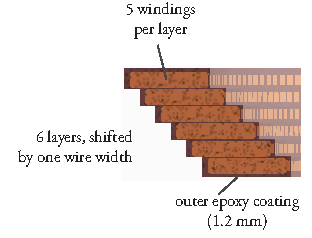
\includegraphics[]{\imagepath/coil_geometry_specification/coil_geometry_specification.pdf}
        \caption{Coil cross-section specification: The six winding layers are arranged in a parallelogram shape, with each layer having 5 windings.}
        \label{fig:coil_geometry_specification}
    \end{subfigure}
    \hspace{0.09\textwidth}
    \begin{subfigure}[t]{0.45\textwidth}
        \centering
        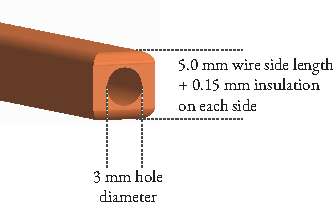
\includegraphics[]{\imagepath/wire_specification/wire_specification.pdf}
        \caption{Wire specification: The square copper wire has a side length of \SI{5.0}{\milli\meter}, the hollow core has a diameter of \SI{3.0}{\milli\meter}. On each side, a Kapton insulation layer of \SI{0.15}{\milli\meter} }
        \label{fig:wire_specification}
    \end{subfigure}
    \caption{Cross-section geometry and wire specification}
\end{figure}

\begin{figure}
    \centering
    \begin{subfigure}[t]{0.48\textwidth}
        \centering
        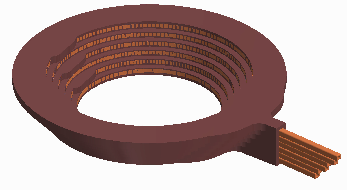
\includegraphics[]{\imagepath/single_coil_drawing/single_coil_drawing.pdf}
        \caption{3-dimensional drawing of a Feshbach coil. The layer jumps connecting the two layers within each pancake sit opposite of the supply lines.\todo[inline]{check, makes sense?}} 
        \label{fig:single_coil_drawing}
    \end{subfigure}
    \hspace{0.03\textwidth}
    \begin{subfigure}[t]{0.48\textwidth}
        \centering
        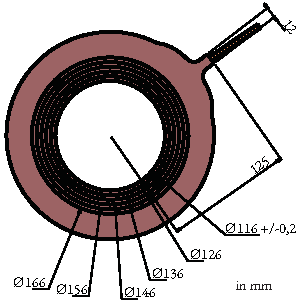
\includegraphics[]{\imagepath/single_coil_geometry_kraemer/single_coil_geometry_kraemer.pdf}
        \caption{Specified geometrical properties of the Feshbach coils. Drawing supplied by the producer (Krämer Energietechnik)}
        \label{fig:single_coil_geometry_kraemer}
    \end{subfigure}
    \caption{Geometry of a Feshbach coil}
\end{figure}

The coils are held in place using holders designed by the engineering department of the Max Planck Institute of Quantum Optics, made out of the non-magnetic material PEEK. Massive spacers between the two coils ensure that they cannot change their distance due to any gradient forces, and they impede vibrations by tightly fixing the coils.

\subsection*{Operational Properties}
The operational properties introduced in section \ref{ch:simulation} were simulated using the \textit{coil simulation library} and are listed in table~\ref{tab:operational_properties}.

\begin{table}
    \centering
    \begin{tabular}{rcc}
        \toprule
        quantity & simulated value  & equation reference \\
        \toprule
        wire length & \SI{15.7}{\meter} & \\
        resistance $R_\mathcal{L}$ & \SI{15.7}{\milli\ohm} & \eqref{eq:resistance_simulation} \\
        \midrule
        inductance $L_\mathcal{L}$ (single coil) & \SI{0.15}{\milli\henry} & \multirow{3}{*}{\eqref{eq:inductance_simulation}} \\ 
        inductance $L_\mathcal{L}$ (Helmholtz configuration) & \SI{0.20}{\milli\henry} & \\ 
        inductance $L_\mathcal{L}$ (gradient configuration) & \SI{0.10}{\milli\henry} & \\ 
        \midrule
        time constant $\tau_\mathcal{L}$ (single coil) & \SI{9.9}{\milli\second} & \multirow{3}{*}{\eqref{eq:time_constant_simulation}}\\
        time constant $\tau_\mathcal{L}$ (Helmholtz configuration) & \SI{13.3}{\milli\second} & \\
        time constant $\tau_\mathcal{L}$ (gradient configuration) & \SI{6.5}{\milli\second} & \\
        \bottomrule
    \end{tabular}
    \caption{Operational properties of the Feshbach coils determined using the \text{coil simulation library}}
    \label{tab:operational_properties}
\end{table}

\todo{add resonance and resistance measurements}

\subsection*{Magnetic Fields}
Using a Sensys FGM3D/1000 fluxgate magnetic field probe (dominant relative error of \SI{0.5}{\percent}), the on-axis magnetic field produced by the three coils \textit{Gauss}, \textit{Maxwell}, and \textit{Tesla} at $I = \SI{1.000}{\ampere}$ was mapped and is displayed in figure~\ref{fig:single_coil_fields}. In addition to that, the fields were fit to the following model the on-axis field of \SI{30}{} partially separated wire loops:
\begin{align}\label{eq:on_axis_field_model}
    \hat B(I, r, y_0) = \sum\limits_{a = 0}^5 \sum\limits_{c = 0}^4 \frac{\mu_0 I}{2} \frac{r_{ac}^2}{\left(r_{ac}^2 + y_{ac}^2\right)^\frac{3}{2}}
\end{align}
with the $y$ position $y_{ac} = y_0 + (a - 2.5) w$ and the radius $r_{ac} = r + (c-2)w$ of a winding with on-axis index $a$, cross-axis index $c$, and a winding spacing $w$.

With root means square error $RMSE[B, \hat B] = \sqrt{\frac{1}{N}\sum_{i = 1}^N (B_i-\hat B_i)^2}$ values of $<\SI{3}{\milli\gauss}$, which is about \SI{e-3}{} of the maximum field, the model fits the observed field landscapes very well. The resulting parameters $\hat I$, $\hat r$, and $\hat y_0$ are listed in table~\ref{tab:single_coil_fields_fit_parameters}.\footnote{$\hat I$ and $\hat r$ are highly correlated (\SI{99.9976}{\percent}), which can be attributed to $\hat B \underset{y^2 \ll r^2}{\propto} \frac{I}{r}$. This means that } One can conclude that the coils cannot produce the same maximum field and that they act like they are operated at different currents and/or have slightly different dimensions. Comparing the measured and the simulated fields with $RMSE[B, B_\text{simulated}]$ (see table~\ref{tab:single_coil_fields_fit_parameters}), one can also see that \textit{Tesla} matches the expected field landscape best, followed by \textit{Gauss}, and \textit{Maxwell} very far off.

\begin{figure}
    \centering
    \begin{pgfpicture}
        \pgftext{%% Creator: Matplotlib, PGF backend
%%
%% To include the figure in your LaTeX document, write
%%   \input{<filename>.pgf}
%%
%% Make sure the required packages are loaded in your preamble
%%   \usepackage{pgf}
%%
%% Also ensure that all the required font packages are loaded; for instance,
%% the lmodern package is sometimes necessary when using math font.
%%   \usepackage{lmodern}
%%
%% Figures using additional raster images can only be included by \input if
%% they are in the same directory as the main LaTeX file. For loading figures
%% from other directories you can use the `import` package
%%   \usepackage{import}
%%
%% and then include the figures with
%%   \import{<path to file>}{<filename>.pgf}
%%
%% Matplotlib used the following preamble
%%   \usepackage{fontspec}
%%   \setmainfont{DejaVuSerif.ttf}[Path=\detokenize{/home/max/.conda/envs/3d_mot/lib/python3.9/site-packages/matplotlib/mpl-data/fonts/ttf/}]
%%   \setsansfont{DejaVuSans.ttf}[Path=\detokenize{/home/max/.conda/envs/3d_mot/lib/python3.9/site-packages/matplotlib/mpl-data/fonts/ttf/}]
%%   \setmonofont{DejaVuSansMono.ttf}[Path=\detokenize{/home/max/.conda/envs/3d_mot/lib/python3.9/site-packages/matplotlib/mpl-data/fonts/ttf/}]
%%
\begingroup%
\makeatletter%
\begin{pgfpicture}%
\pgfpathrectangle{\pgfpointorigin}{\pgfqpoint{5.830290in}{2.677849in}}%
\pgfusepath{use as bounding box, clip}%
\begin{pgfscope}%
\pgfsetbuttcap%
\pgfsetmiterjoin%
\pgfsetlinewidth{0.000000pt}%
\definecolor{currentstroke}{rgb}{1.000000,1.000000,1.000000}%
\pgfsetstrokecolor{currentstroke}%
\pgfsetstrokeopacity{0.000000}%
\pgfsetdash{}{0pt}%
\pgfpathmoveto{\pgfqpoint{0.000000in}{0.000000in}}%
\pgfpathlineto{\pgfqpoint{5.830290in}{0.000000in}}%
\pgfpathlineto{\pgfqpoint{5.830290in}{2.677849in}}%
\pgfpathlineto{\pgfqpoint{0.000000in}{2.677849in}}%
\pgfpathlineto{\pgfqpoint{0.000000in}{0.000000in}}%
\pgfpathclose%
\pgfusepath{}%
\end{pgfscope}%
\begin{pgfscope}%
\pgfsetbuttcap%
\pgfsetmiterjoin%
\definecolor{currentfill}{rgb}{1.000000,1.000000,1.000000}%
\pgfsetfillcolor{currentfill}%
\pgfsetlinewidth{0.000000pt}%
\definecolor{currentstroke}{rgb}{0.000000,0.000000,0.000000}%
\pgfsetstrokecolor{currentstroke}%
\pgfsetstrokeopacity{0.000000}%
\pgfsetdash{}{0pt}%
\pgfpathmoveto{\pgfqpoint{0.652070in}{0.494721in}}%
\pgfpathlineto{\pgfqpoint{5.730290in}{0.494721in}}%
\pgfpathlineto{\pgfqpoint{5.730290in}{2.577849in}}%
\pgfpathlineto{\pgfqpoint{0.652070in}{2.577849in}}%
\pgfpathlineto{\pgfqpoint{0.652070in}{0.494721in}}%
\pgfpathclose%
\pgfusepath{fill}%
\end{pgfscope}%
\begin{pgfscope}%
\pgfpathrectangle{\pgfqpoint{0.652070in}{0.494721in}}{\pgfqpoint{5.078220in}{2.083128in}}%
\pgfusepath{clip}%
\pgfsetbuttcap%
\pgfsetroundjoin%
\definecolor{currentfill}{rgb}{0.313725,0.741176,0.913725}%
\pgfsetfillcolor{currentfill}%
\pgfsetlinewidth{1.505625pt}%
\definecolor{currentstroke}{rgb}{0.313725,0.741176,0.913725}%
\pgfsetstrokecolor{currentstroke}%
\pgfsetdash{}{0pt}%
\pgfsys@defobject{currentmarker}{\pgfqpoint{-0.021960in}{-0.021960in}}{\pgfqpoint{0.021960in}{0.021960in}}{%
\pgfpathmoveto{\pgfqpoint{-0.021960in}{-0.021960in}}%
\pgfpathlineto{\pgfqpoint{0.021960in}{0.021960in}}%
\pgfpathmoveto{\pgfqpoint{-0.021960in}{0.021960in}}%
\pgfpathlineto{\pgfqpoint{0.021960in}{-0.021960in}}%
\pgfusepath{stroke,fill}%
}%
\begin{pgfscope}%
\pgfsys@transformshift{1.190787in}{2.212826in}%
\pgfsys@useobject{currentmarker}{}%
\end{pgfscope}%
\begin{pgfscope}%
\pgfsys@transformshift{1.230561in}{2.233834in}%
\pgfsys@useobject{currentmarker}{}%
\end{pgfscope}%
\begin{pgfscope}%
\pgfsys@transformshift{1.260391in}{2.247102in}%
\pgfsys@useobject{currentmarker}{}%
\end{pgfscope}%
\begin{pgfscope}%
\pgfsys@transformshift{1.296613in}{2.265898in}%
\pgfsys@useobject{currentmarker}{}%
\end{pgfscope}%
\begin{pgfscope}%
\pgfsys@transformshift{1.332125in}{2.284694in}%
\pgfsys@useobject{currentmarker}{}%
\end{pgfscope}%
\begin{pgfscope}%
\pgfsys@transformshift{1.367282in}{2.296856in}%
\pgfsys@useobject{currentmarker}{}%
\end{pgfscope}%
\begin{pgfscope}%
\pgfsys@transformshift{1.402439in}{2.310124in}%
\pgfsys@useobject{currentmarker}{}%
\end{pgfscope}%
\begin{pgfscope}%
\pgfsys@transformshift{1.440082in}{2.325603in}%
\pgfsys@useobject{currentmarker}{}%
\end{pgfscope}%
\begin{pgfscope}%
\pgfsys@transformshift{1.472753in}{2.337765in}%
\pgfsys@useobject{currentmarker}{}%
\end{pgfscope}%
\begin{pgfscope}%
\pgfsys@transformshift{1.511106in}{2.352139in}%
\pgfsys@useobject{currentmarker}{}%
\end{pgfscope}%
\begin{pgfscope}%
\pgfsys@transformshift{1.544487in}{2.362090in}%
\pgfsys@useobject{currentmarker}{}%
\end{pgfscope}%
\begin{pgfscope}%
\pgfsys@transformshift{1.581064in}{2.372041in}%
\pgfsys@useobject{currentmarker}{}%
\end{pgfscope}%
\begin{pgfscope}%
\pgfsys@transformshift{1.619417in}{2.383097in}%
\pgfsys@useobject{currentmarker}{}%
\end{pgfscope}%
\begin{pgfscope}%
\pgfsys@transformshift{1.653864in}{2.391942in}%
\pgfsys@useobject{currentmarker}{}%
\end{pgfscope}%
\begin{pgfscope}%
\pgfsys@transformshift{1.686535in}{2.398576in}%
\pgfsys@useobject{currentmarker}{}%
\end{pgfscope}%
\begin{pgfscope}%
\pgfsys@transformshift{1.721692in}{2.406316in}%
\pgfsys@useobject{currentmarker}{}%
\end{pgfscope}%
\begin{pgfscope}%
\pgfsys@transformshift{1.756849in}{2.411844in}%
\pgfsys@useobject{currentmarker}{}%
\end{pgfscope}%
\begin{pgfscope}%
\pgfsys@transformshift{1.793426in}{2.417373in}%
\pgfsys@useobject{currentmarker}{}%
\end{pgfscope}%
\begin{pgfscope}%
\pgfsys@transformshift{1.831424in}{2.420689in}%
\pgfsys@useobject{currentmarker}{}%
\end{pgfscope}%
\begin{pgfscope}%
\pgfsys@transformshift{1.865160in}{2.425112in}%
\pgfsys@useobject{currentmarker}{}%
\end{pgfscope}%
\begin{pgfscope}%
\pgfsys@transformshift{1.901383in}{2.426218in}%
\pgfsys@useobject{currentmarker}{}%
\end{pgfscope}%
\begin{pgfscope}%
\pgfsys@transformshift{1.935119in}{2.426218in}%
\pgfsys@useobject{currentmarker}{}%
\end{pgfscope}%
\begin{pgfscope}%
\pgfsys@transformshift{1.971341in}{2.426218in}%
\pgfsys@useobject{currentmarker}{}%
\end{pgfscope}%
\begin{pgfscope}%
\pgfsys@transformshift{2.006853in}{2.426218in}%
\pgfsys@useobject{currentmarker}{}%
\end{pgfscope}%
\begin{pgfscope}%
\pgfsys@transformshift{2.043431in}{2.422901in}%
\pgfsys@useobject{currentmarker}{}%
\end{pgfscope}%
\begin{pgfscope}%
\pgfsys@transformshift{2.080363in}{2.419584in}%
\pgfsys@useobject{currentmarker}{}%
\end{pgfscope}%
\begin{pgfscope}%
\pgfsys@transformshift{2.112679in}{2.416267in}%
\pgfsys@useobject{currentmarker}{}%
\end{pgfscope}%
\begin{pgfscope}%
\pgfsys@transformshift{2.148902in}{2.410739in}%
\pgfsys@useobject{currentmarker}{}%
\end{pgfscope}%
\begin{pgfscope}%
\pgfsys@transformshift{2.183348in}{2.402999in}%
\pgfsys@useobject{currentmarker}{}%
\end{pgfscope}%
\begin{pgfscope}%
\pgfsys@transformshift{2.220281in}{2.397471in}%
\pgfsys@useobject{currentmarker}{}%
\end{pgfscope}%
\begin{pgfscope}%
\pgfsys@transformshift{2.256858in}{2.388625in}%
\pgfsys@useobject{currentmarker}{}%
\end{pgfscope}%
\begin{pgfscope}%
\pgfsys@transformshift{2.293436in}{2.377569in}%
\pgfsys@useobject{currentmarker}{}%
\end{pgfscope}%
\begin{pgfscope}%
\pgfsys@transformshift{2.327172in}{2.367618in}%
\pgfsys@useobject{currentmarker}{}%
\end{pgfscope}%
\begin{pgfscope}%
\pgfsys@transformshift{2.361264in}{2.357667in}%
\pgfsys@useobject{currentmarker}{}%
\end{pgfscope}%
\begin{pgfscope}%
\pgfsys@transformshift{2.399972in}{2.344399in}%
\pgfsys@useobject{currentmarker}{}%
\end{pgfscope}%
\begin{pgfscope}%
\pgfsys@transformshift{2.436549in}{2.331131in}%
\pgfsys@useobject{currentmarker}{}%
\end{pgfscope}%
\begin{pgfscope}%
\pgfsys@transformshift{2.467800in}{2.318969in}%
\pgfsys@useobject{currentmarker}{}%
\end{pgfscope}%
\begin{pgfscope}%
\pgfsys@transformshift{2.505087in}{2.302384in}%
\pgfsys@useobject{currentmarker}{}%
\end{pgfscope}%
\begin{pgfscope}%
\pgfsys@transformshift{2.539179in}{2.286905in}%
\pgfsys@useobject{currentmarker}{}%
\end{pgfscope}%
\begin{pgfscope}%
\pgfsys@transformshift{2.577177in}{2.270320in}%
\pgfsys@useobject{currentmarker}{}%
\end{pgfscope}%
\begin{pgfscope}%
\pgfsys@transformshift{2.610203in}{2.252630in}%
\pgfsys@useobject{currentmarker}{}%
\end{pgfscope}%
\begin{pgfscope}%
\pgfsys@transformshift{2.645715in}{2.234939in}%
\pgfsys@useobject{currentmarker}{}%
\end{pgfscope}%
\begin{pgfscope}%
\pgfsys@transformshift{2.683713in}{2.215038in}%
\pgfsys@useobject{currentmarker}{}%
\end{pgfscope}%
\begin{pgfscope}%
\pgfsys@transformshift{2.720645in}{2.194030in}%
\pgfsys@useobject{currentmarker}{}%
\end{pgfscope}%
\begin{pgfscope}%
\pgfsys@transformshift{2.751896in}{2.177445in}%
\pgfsys@useobject{currentmarker}{}%
\end{pgfscope}%
\begin{pgfscope}%
\pgfsys@transformshift{2.787053in}{2.155332in}%
\pgfsys@useobject{currentmarker}{}%
\end{pgfscope}%
\begin{pgfscope}%
\pgfsys@transformshift{2.822565in}{2.134325in}%
\pgfsys@useobject{currentmarker}{}%
\end{pgfscope}%
\begin{pgfscope}%
\pgfsys@transformshift{2.857722in}{2.111106in}%
\pgfsys@useobject{currentmarker}{}%
\end{pgfscope}%
\begin{pgfscope}%
\pgfsys@transformshift{2.896075in}{2.087887in}%
\pgfsys@useobject{currentmarker}{}%
\end{pgfscope}%
\begin{pgfscope}%
\pgfsys@transformshift{2.933007in}{2.066880in}%
\pgfsys@useobject{currentmarker}{}%
\end{pgfscope}%
\begin{pgfscope}%
\pgfsys@transformshift{2.964968in}{2.044767in}%
\pgfsys@useobject{currentmarker}{}%
\end{pgfscope}%
\begin{pgfscope}%
\pgfsys@transformshift{3.001190in}{2.020442in}%
\pgfsys@useobject{currentmarker}{}%
\end{pgfscope}%
\begin{pgfscope}%
\pgfsys@transformshift{3.035282in}{1.999435in}%
\pgfsys@useobject{currentmarker}{}%
\end{pgfscope}%
\begin{pgfscope}%
\pgfsys@transformshift{3.071149in}{1.974005in}%
\pgfsys@useobject{currentmarker}{}%
\end{pgfscope}%
\begin{pgfscope}%
\pgfsys@transformshift{3.105951in}{1.949680in}%
\pgfsys@useobject{currentmarker}{}%
\end{pgfscope}%
\begin{pgfscope}%
\pgfsys@transformshift{3.141463in}{1.926462in}%
\pgfsys@useobject{currentmarker}{}%
\end{pgfscope}%
\begin{pgfscope}%
\pgfsys@transformshift{3.181591in}{1.895503in}%
\pgfsys@useobject{currentmarker}{}%
\end{pgfscope}%
\begin{pgfscope}%
\pgfsys@transformshift{3.214973in}{1.871179in}%
\pgfsys@useobject{currentmarker}{}%
\end{pgfscope}%
\begin{pgfscope}%
\pgfsys@transformshift{3.254391in}{1.844643in}%
\pgfsys@useobject{currentmarker}{}%
\end{pgfscope}%
\begin{pgfscope}%
\pgfsys@transformshift{3.285287in}{1.819213in}%
\pgfsys@useobject{currentmarker}{}%
\end{pgfscope}%
\begin{pgfscope}%
\pgfsys@transformshift{3.320443in}{1.797100in}%
\pgfsys@useobject{currentmarker}{}%
\end{pgfscope}%
\begin{pgfscope}%
\pgfsys@transformshift{3.354535in}{1.771670in}%
\pgfsys@useobject{currentmarker}{}%
\end{pgfscope}%
\begin{pgfscope}%
\pgfsys@transformshift{3.392888in}{1.744029in}%
\pgfsys@useobject{currentmarker}{}%
\end{pgfscope}%
\begin{pgfscope}%
\pgfsys@transformshift{3.428045in}{1.717493in}%
\pgfsys@useobject{currentmarker}{}%
\end{pgfscope}%
\begin{pgfscope}%
\pgfsys@transformshift{3.463912in}{1.688746in}%
\pgfsys@useobject{currentmarker}{}%
\end{pgfscope}%
\begin{pgfscope}%
\pgfsys@transformshift{3.498714in}{1.664421in}%
\pgfsys@useobject{currentmarker}{}%
\end{pgfscope}%
\begin{pgfscope}%
\pgfsys@transformshift{3.536001in}{1.638991in}%
\pgfsys@useobject{currentmarker}{}%
\end{pgfscope}%
\begin{pgfscope}%
\pgfsys@transformshift{3.571869in}{1.611350in}%
\pgfsys@useobject{currentmarker}{}%
\end{pgfscope}%
\begin{pgfscope}%
\pgfsys@transformshift{3.605960in}{1.587026in}%
\pgfsys@useobject{currentmarker}{}%
\end{pgfscope}%
\begin{pgfscope}%
\pgfsys@transformshift{3.643248in}{1.561595in}%
\pgfsys@useobject{currentmarker}{}%
\end{pgfscope}%
\begin{pgfscope}%
\pgfsys@transformshift{3.680535in}{1.532848in}%
\pgfsys@useobject{currentmarker}{}%
\end{pgfscope}%
\begin{pgfscope}%
\pgfsys@transformshift{3.711786in}{1.511841in}%
\pgfsys@useobject{currentmarker}{}%
\end{pgfscope}%
\begin{pgfscope}%
\pgfsys@transformshift{3.747653in}{1.484200in}%
\pgfsys@useobject{currentmarker}{}%
\end{pgfscope}%
\begin{pgfscope}%
\pgfsys@transformshift{3.784586in}{1.460981in}%
\pgfsys@useobject{currentmarker}{}%
\end{pgfscope}%
\begin{pgfscope}%
\pgfsys@transformshift{3.820808in}{1.433339in}%
\pgfsys@useobject{currentmarker}{}%
\end{pgfscope}%
\begin{pgfscope}%
\pgfsys@transformshift{3.855965in}{1.409015in}%
\pgfsys@useobject{currentmarker}{}%
\end{pgfscope}%
\begin{pgfscope}%
\pgfsys@transformshift{3.889701in}{1.385796in}%
\pgfsys@useobject{currentmarker}{}%
\end{pgfscope}%
\begin{pgfscope}%
\pgfsys@transformshift{3.928409in}{1.359261in}%
\pgfsys@useobject{currentmarker}{}%
\end{pgfscope}%
\begin{pgfscope}%
\pgfsys@transformshift{3.963921in}{1.334936in}%
\pgfsys@useobject{currentmarker}{}%
\end{pgfscope}%
\begin{pgfscope}%
\pgfsys@transformshift{4.001209in}{1.308400in}%
\pgfsys@useobject{currentmarker}{}%
\end{pgfscope}%
\begin{pgfscope}%
\pgfsys@transformshift{4.038497in}{1.286287in}%
\pgfsys@useobject{currentmarker}{}%
\end{pgfscope}%
\begin{pgfscope}%
\pgfsys@transformshift{4.070457in}{1.266386in}%
\pgfsys@useobject{currentmarker}{}%
\end{pgfscope}%
\begin{pgfscope}%
\pgfsys@transformshift{4.107035in}{1.242061in}%
\pgfsys@useobject{currentmarker}{}%
\end{pgfscope}%
\begin{pgfscope}%
\pgfsys@transformshift{4.138641in}{1.223265in}%
\pgfsys@useobject{currentmarker}{}%
\end{pgfscope}%
\begin{pgfscope}%
\pgfsys@transformshift{4.175573in}{1.198941in}%
\pgfsys@useobject{currentmarker}{}%
\end{pgfscope}%
\begin{pgfscope}%
\pgfsys@transformshift{4.210020in}{1.177933in}%
\pgfsys@useobject{currentmarker}{}%
\end{pgfscope}%
\begin{pgfscope}%
\pgfsys@transformshift{4.249438in}{1.154714in}%
\pgfsys@useobject{currentmarker}{}%
\end{pgfscope}%
\begin{pgfscope}%
\pgfsys@transformshift{4.283885in}{1.134813in}%
\pgfsys@useobject{currentmarker}{}%
\end{pgfscope}%
\begin{pgfscope}%
\pgfsys@transformshift{4.318331in}{1.114911in}%
\pgfsys@useobject{currentmarker}{}%
\end{pgfscope}%
\begin{pgfscope}%
\pgfsys@transformshift{4.351003in}{1.092798in}%
\pgfsys@useobject{currentmarker}{}%
\end{pgfscope}%
\begin{pgfscope}%
\pgfsys@transformshift{4.390066in}{1.071790in}%
\pgfsys@useobject{currentmarker}{}%
\end{pgfscope}%
\begin{pgfscope}%
\pgfsys@transformshift{4.419186in}{1.051888in}%
\pgfsys@useobject{currentmarker}{}%
\end{pgfscope}%
\begin{pgfscope}%
\pgfsys@transformshift{4.461445in}{1.033092in}%
\pgfsys@useobject{currentmarker}{}%
\end{pgfscope}%
\begin{pgfscope}%
\pgfsys@transformshift{4.496957in}{1.014296in}%
\pgfsys@useobject{currentmarker}{}%
\end{pgfscope}%
\begin{pgfscope}%
\pgfsys@transformshift{4.529983in}{0.997711in}%
\pgfsys@useobject{currentmarker}{}%
\end{pgfscope}%
\begin{pgfscope}%
\pgfsys@transformshift{4.565495in}{0.978915in}%
\pgfsys@useobject{currentmarker}{}%
\end{pgfscope}%
\begin{pgfscope}%
\pgfsys@transformshift{4.599942in}{0.961225in}%
\pgfsys@useobject{currentmarker}{}%
\end{pgfscope}%
\begin{pgfscope}%
\pgfsys@transformshift{4.639360in}{0.940217in}%
\pgfsys@useobject{currentmarker}{}%
\end{pgfscope}%
\begin{pgfscope}%
\pgfsys@transformshift{4.674872in}{0.922527in}%
\pgfsys@useobject{currentmarker}{}%
\end{pgfscope}%
\begin{pgfscope}%
\pgfsys@transformshift{4.711450in}{0.902625in}%
\pgfsys@useobject{currentmarker}{}%
\end{pgfscope}%
\begin{pgfscope}%
\pgfsys@transformshift{4.741280in}{0.889357in}%
\pgfsys@useobject{currentmarker}{}%
\end{pgfscope}%
\begin{pgfscope}%
\pgfsys@transformshift{4.782829in}{0.869455in}%
\pgfsys@useobject{currentmarker}{}%
\end{pgfscope}%
\begin{pgfscope}%
\pgfsys@transformshift{4.811949in}{0.856187in}%
\pgfsys@useobject{currentmarker}{}%
\end{pgfscope}%
\begin{pgfscope}%
\pgfsys@transformshift{4.851367in}{0.838497in}%
\pgfsys@useobject{currentmarker}{}%
\end{pgfscope}%
\begin{pgfscope}%
\pgfsys@transformshift{4.890075in}{0.820807in}%
\pgfsys@useobject{currentmarker}{}%
\end{pgfscope}%
\begin{pgfscope}%
\pgfsys@transformshift{4.918840in}{0.811961in}%
\pgfsys@useobject{currentmarker}{}%
\end{pgfscope}%
\begin{pgfscope}%
\pgfsys@transformshift{4.956127in}{0.793165in}%
\pgfsys@useobject{currentmarker}{}%
\end{pgfscope}%
\begin{pgfscope}%
\pgfsys@transformshift{4.993060in}{0.776580in}%
\pgfsys@useobject{currentmarker}{}%
\end{pgfscope}%
\begin{pgfscope}%
\pgfsys@transformshift{5.026441in}{0.763312in}%
\pgfsys@useobject{currentmarker}{}%
\end{pgfscope}%
\begin{pgfscope}%
\pgfsys@transformshift{5.063019in}{0.748939in}%
\pgfsys@useobject{currentmarker}{}%
\end{pgfscope}%
\end{pgfscope}%
\begin{pgfscope}%
\pgfpathrectangle{\pgfqpoint{0.652070in}{0.494721in}}{\pgfqpoint{5.078220in}{2.083128in}}%
\pgfusepath{clip}%
\pgfsetbuttcap%
\pgfsetroundjoin%
\definecolor{currentfill}{rgb}{0.603922,0.356863,0.568627}%
\pgfsetfillcolor{currentfill}%
\pgfsetlinewidth{1.505625pt}%
\definecolor{currentstroke}{rgb}{0.603922,0.356863,0.568627}%
\pgfsetstrokecolor{currentstroke}%
\pgfsetdash{}{0pt}%
\pgfsys@defobject{currentmarker}{\pgfqpoint{-0.021960in}{-0.021960in}}{\pgfqpoint{0.021960in}{0.021960in}}{%
\pgfpathmoveto{\pgfqpoint{-0.021960in}{-0.021960in}}%
\pgfpathlineto{\pgfqpoint{0.021960in}{0.021960in}}%
\pgfpathmoveto{\pgfqpoint{-0.021960in}{0.021960in}}%
\pgfpathlineto{\pgfqpoint{0.021960in}{-0.021960in}}%
\pgfusepath{stroke,fill}%
}%
\begin{pgfscope}%
\pgfsys@transformshift{1.168414in}{2.090099in}%
\pgfsys@useobject{currentmarker}{}%
\end{pgfscope}%
\begin{pgfscope}%
\pgfsys@transformshift{1.204992in}{2.108895in}%
\pgfsys@useobject{currentmarker}{}%
\end{pgfscope}%
\begin{pgfscope}%
\pgfsys@transformshift{1.240504in}{2.125480in}%
\pgfsys@useobject{currentmarker}{}%
\end{pgfscope}%
\begin{pgfscope}%
\pgfsys@transformshift{1.276016in}{2.139853in}%
\pgfsys@useobject{currentmarker}{}%
\end{pgfscope}%
\begin{pgfscope}%
\pgfsys@transformshift{1.309397in}{2.155332in}%
\pgfsys@useobject{currentmarker}{}%
\end{pgfscope}%
\begin{pgfscope}%
\pgfsys@transformshift{1.344909in}{2.169706in}%
\pgfsys@useobject{currentmarker}{}%
\end{pgfscope}%
\begin{pgfscope}%
\pgfsys@transformshift{1.383262in}{2.186291in}%
\pgfsys@useobject{currentmarker}{}%
\end{pgfscope}%
\begin{pgfscope}%
\pgfsys@transformshift{1.416999in}{2.197347in}%
\pgfsys@useobject{currentmarker}{}%
\end{pgfscope}%
\begin{pgfscope}%
\pgfsys@transformshift{1.453931in}{2.210615in}%
\pgfsys@useobject{currentmarker}{}%
\end{pgfscope}%
\begin{pgfscope}%
\pgfsys@transformshift{1.490509in}{2.222777in}%
\pgfsys@useobject{currentmarker}{}%
\end{pgfscope}%
\begin{pgfscope}%
\pgfsys@transformshift{1.522825in}{2.232728in}%
\pgfsys@useobject{currentmarker}{}%
\end{pgfscope}%
\begin{pgfscope}%
\pgfsys@transformshift{1.559757in}{2.243785in}%
\pgfsys@useobject{currentmarker}{}%
\end{pgfscope}%
\begin{pgfscope}%
\pgfsys@transformshift{1.596334in}{2.251524in}%
\pgfsys@useobject{currentmarker}{}%
\end{pgfscope}%
\begin{pgfscope}%
\pgfsys@transformshift{1.630781in}{2.260369in}%
\pgfsys@useobject{currentmarker}{}%
\end{pgfscope}%
\begin{pgfscope}%
\pgfsys@transformshift{1.665583in}{2.268109in}%
\pgfsys@useobject{currentmarker}{}%
\end{pgfscope}%
\begin{pgfscope}%
\pgfsys@transformshift{1.700740in}{2.274743in}%
\pgfsys@useobject{currentmarker}{}%
\end{pgfscope}%
\begin{pgfscope}%
\pgfsys@transformshift{1.742289in}{2.281377in}%
\pgfsys@useobject{currentmarker}{}%
\end{pgfscope}%
\begin{pgfscope}%
\pgfsys@transformshift{1.771409in}{2.285800in}%
\pgfsys@useobject{currentmarker}{}%
\end{pgfscope}%
\begin{pgfscope}%
\pgfsys@transformshift{1.806921in}{2.286905in}%
\pgfsys@useobject{currentmarker}{}%
\end{pgfscope}%
\begin{pgfscope}%
\pgfsys@transformshift{1.843498in}{2.292433in}%
\pgfsys@useobject{currentmarker}{}%
\end{pgfscope}%
\begin{pgfscope}%
\pgfsys@transformshift{1.877945in}{2.294645in}%
\pgfsys@useobject{currentmarker}{}%
\end{pgfscope}%
\begin{pgfscope}%
\pgfsys@transformshift{1.913102in}{2.295750in}%
\pgfsys@useobject{currentmarker}{}%
\end{pgfscope}%
\begin{pgfscope}%
\pgfsys@transformshift{1.949324in}{2.295750in}%
\pgfsys@useobject{currentmarker}{}%
\end{pgfscope}%
\begin{pgfscope}%
\pgfsys@transformshift{1.985546in}{2.294645in}%
\pgfsys@useobject{currentmarker}{}%
\end{pgfscope}%
\begin{pgfscope}%
\pgfsys@transformshift{2.021058in}{2.292433in}%
\pgfsys@useobject{currentmarker}{}%
\end{pgfscope}%
\begin{pgfscope}%
\pgfsys@transformshift{2.057281in}{2.290222in}%
\pgfsys@useobject{currentmarker}{}%
\end{pgfscope}%
\begin{pgfscope}%
\pgfsys@transformshift{2.092793in}{2.286905in}%
\pgfsys@useobject{currentmarker}{}%
\end{pgfscope}%
\begin{pgfscope}%
\pgfsys@transformshift{2.127594in}{2.281377in}%
\pgfsys@useobject{currentmarker}{}%
\end{pgfscope}%
\begin{pgfscope}%
\pgfsys@transformshift{2.163817in}{2.275849in}%
\pgfsys@useobject{currentmarker}{}%
\end{pgfscope}%
\begin{pgfscope}%
\pgfsys@transformshift{2.199684in}{2.268109in}%
\pgfsys@useobject{currentmarker}{}%
\end{pgfscope}%
\begin{pgfscope}%
\pgfsys@transformshift{2.234841in}{2.261475in}%
\pgfsys@useobject{currentmarker}{}%
\end{pgfscope}%
\begin{pgfscope}%
\pgfsys@transformshift{2.270353in}{2.252630in}%
\pgfsys@useobject{currentmarker}{}%
\end{pgfscope}%
\begin{pgfscope}%
\pgfsys@transformshift{2.305155in}{2.244890in}%
\pgfsys@useobject{currentmarker}{}%
\end{pgfscope}%
\begin{pgfscope}%
\pgfsys@transformshift{2.339246in}{2.234939in}%
\pgfsys@useobject{currentmarker}{}%
\end{pgfscope}%
\begin{pgfscope}%
\pgfsys@transformshift{2.374403in}{2.222777in}%
\pgfsys@useobject{currentmarker}{}%
\end{pgfscope}%
\begin{pgfscope}%
\pgfsys@transformshift{2.411335in}{2.210615in}%
\pgfsys@useobject{currentmarker}{}%
\end{pgfscope}%
\begin{pgfscope}%
\pgfsys@transformshift{2.446848in}{2.197347in}%
\pgfsys@useobject{currentmarker}{}%
\end{pgfscope}%
\begin{pgfscope}%
\pgfsys@transformshift{2.484845in}{2.182974in}%
\pgfsys@useobject{currentmarker}{}%
\end{pgfscope}%
\begin{pgfscope}%
\pgfsys@transformshift{2.518582in}{2.168600in}%
\pgfsys@useobject{currentmarker}{}%
\end{pgfscope}%
\begin{pgfscope}%
\pgfsys@transformshift{2.558710in}{2.152015in}%
\pgfsys@useobject{currentmarker}{}%
\end{pgfscope}%
\begin{pgfscope}%
\pgfsys@transformshift{2.590671in}{2.137642in}%
\pgfsys@useobject{currentmarker}{}%
\end{pgfscope}%
\begin{pgfscope}%
\pgfsys@transformshift{2.625473in}{2.121057in}%
\pgfsys@useobject{currentmarker}{}%
\end{pgfscope}%
\begin{pgfscope}%
\pgfsys@transformshift{2.659209in}{2.104472in}%
\pgfsys@useobject{currentmarker}{}%
\end{pgfscope}%
\begin{pgfscope}%
\pgfsys@transformshift{2.695077in}{2.083465in}%
\pgfsys@useobject{currentmarker}{}%
\end{pgfscope}%
\begin{pgfscope}%
\pgfsys@transformshift{2.735560in}{2.065774in}%
\pgfsys@useobject{currentmarker}{}%
\end{pgfscope}%
\begin{pgfscope}%
\pgfsys@transformshift{2.768587in}{2.048084in}%
\pgfsys@useobject{currentmarker}{}%
\end{pgfscope}%
\begin{pgfscope}%
\pgfsys@transformshift{2.801968in}{2.028182in}%
\pgfsys@useobject{currentmarker}{}%
\end{pgfscope}%
\begin{pgfscope}%
\pgfsys@transformshift{2.839255in}{2.008280in}%
\pgfsys@useobject{currentmarker}{}%
\end{pgfscope}%
\begin{pgfscope}%
\pgfsys@transformshift{2.871571in}{1.988378in}%
\pgfsys@useobject{currentmarker}{}%
\end{pgfscope}%
\begin{pgfscope}%
\pgfsys@transformshift{2.909214in}{1.966265in}%
\pgfsys@useobject{currentmarker}{}%
\end{pgfscope}%
\begin{pgfscope}%
\pgfsys@transformshift{2.947567in}{1.943046in}%
\pgfsys@useobject{currentmarker}{}%
\end{pgfscope}%
\begin{pgfscope}%
\pgfsys@transformshift{2.982014in}{1.920933in}%
\pgfsys@useobject{currentmarker}{}%
\end{pgfscope}%
\begin{pgfscope}%
\pgfsys@transformshift{3.017881in}{1.897715in}%
\pgfsys@useobject{currentmarker}{}%
\end{pgfscope}%
\begin{pgfscope}%
\pgfsys@transformshift{3.049487in}{1.877813in}%
\pgfsys@useobject{currentmarker}{}%
\end{pgfscope}%
\begin{pgfscope}%
\pgfsys@transformshift{3.086419in}{1.855700in}%
\pgfsys@useobject{currentmarker}{}%
\end{pgfscope}%
\begin{pgfscope}%
\pgfsys@transformshift{3.122286in}{1.831375in}%
\pgfsys@useobject{currentmarker}{}%
\end{pgfscope}%
\begin{pgfscope}%
\pgfsys@transformshift{3.162415in}{1.803734in}%
\pgfsys@useobject{currentmarker}{}%
\end{pgfscope}%
\begin{pgfscope}%
\pgfsys@transformshift{3.191535in}{1.784938in}%
\pgfsys@useobject{currentmarker}{}%
\end{pgfscope}%
\begin{pgfscope}%
\pgfsys@transformshift{3.226692in}{1.762825in}%
\pgfsys@useobject{currentmarker}{}%
\end{pgfscope}%
\begin{pgfscope}%
\pgfsys@transformshift{3.265045in}{1.735183in}%
\pgfsys@useobject{currentmarker}{}%
\end{pgfscope}%
\begin{pgfscope}%
\pgfsys@transformshift{3.302687in}{1.708648in}%
\pgfsys@useobject{currentmarker}{}%
\end{pgfscope}%
\begin{pgfscope}%
\pgfsys@transformshift{3.334293in}{1.687640in}%
\pgfsys@useobject{currentmarker}{}%
\end{pgfscope}%
\begin{pgfscope}%
\pgfsys@transformshift{3.372291in}{1.659999in}%
\pgfsys@useobject{currentmarker}{}%
\end{pgfscope}%
\begin{pgfscope}%
\pgfsys@transformshift{3.409579in}{1.636780in}%
\pgfsys@useobject{currentmarker}{}%
\end{pgfscope}%
\begin{pgfscope}%
\pgfsys@transformshift{3.445091in}{1.611350in}%
\pgfsys@useobject{currentmarker}{}%
\end{pgfscope}%
\begin{pgfscope}%
\pgfsys@transformshift{3.483444in}{1.587026in}%
\pgfsys@useobject{currentmarker}{}%
\end{pgfscope}%
\begin{pgfscope}%
\pgfsys@transformshift{3.518601in}{1.561595in}%
\pgfsys@useobject{currentmarker}{}%
\end{pgfscope}%
\begin{pgfscope}%
\pgfsys@transformshift{3.552337in}{1.539482in}%
\pgfsys@useobject{currentmarker}{}%
\end{pgfscope}%
\begin{pgfscope}%
\pgfsys@transformshift{3.588914in}{1.515158in}%
\pgfsys@useobject{currentmarker}{}%
\end{pgfscope}%
\begin{pgfscope}%
\pgfsys@transformshift{3.630819in}{1.485305in}%
\pgfsys@useobject{currentmarker}{}%
\end{pgfscope}%
\begin{pgfscope}%
\pgfsys@transformshift{3.658873in}{1.462086in}%
\pgfsys@useobject{currentmarker}{}%
\end{pgfscope}%
\begin{pgfscope}%
\pgfsys@transformshift{3.693675in}{1.443290in}%
\pgfsys@useobject{currentmarker}{}%
\end{pgfscope}%
\begin{pgfscope}%
\pgfsys@transformshift{3.729187in}{1.420072in}%
\pgfsys@useobject{currentmarker}{}%
\end{pgfscope}%
\begin{pgfscope}%
\pgfsys@transformshift{3.771446in}{1.391325in}%
\pgfsys@useobject{currentmarker}{}%
\end{pgfscope}%
\begin{pgfscope}%
\pgfsys@transformshift{3.801987in}{1.371423in}%
\pgfsys@useobject{currentmarker}{}%
\end{pgfscope}%
\begin{pgfscope}%
\pgfsys@transformshift{3.838209in}{1.347098in}%
\pgfsys@useobject{currentmarker}{}%
\end{pgfscope}%
\begin{pgfscope}%
\pgfsys@transformshift{3.872655in}{1.323880in}%
\pgfsys@useobject{currentmarker}{}%
\end{pgfscope}%
\begin{pgfscope}%
\pgfsys@transformshift{3.912074in}{1.300661in}%
\pgfsys@useobject{currentmarker}{}%
\end{pgfscope}%
\begin{pgfscope}%
\pgfsys@transformshift{3.946521in}{1.278548in}%
\pgfsys@useobject{currentmarker}{}%
\end{pgfscope}%
\begin{pgfscope}%
\pgfsys@transformshift{3.983808in}{1.252012in}%
\pgfsys@useobject{currentmarker}{}%
\end{pgfscope}%
\begin{pgfscope}%
\pgfsys@transformshift{4.020386in}{1.233216in}%
\pgfsys@useobject{currentmarker}{}%
\end{pgfscope}%
\begin{pgfscope}%
\pgfsys@transformshift{4.054832in}{1.211103in}%
\pgfsys@useobject{currentmarker}{}%
\end{pgfscope}%
\begin{pgfscope}%
\pgfsys@transformshift{4.084662in}{1.194518in}%
\pgfsys@useobject{currentmarker}{}%
\end{pgfscope}%
\begin{pgfscope}%
\pgfsys@transformshift{4.121240in}{1.170194in}%
\pgfsys@useobject{currentmarker}{}%
\end{pgfscope}%
\begin{pgfscope}%
\pgfsys@transformshift{4.159593in}{1.149186in}%
\pgfsys@useobject{currentmarker}{}%
\end{pgfscope}%
\begin{pgfscope}%
\pgfsys@transformshift{4.197591in}{1.128179in}%
\pgfsys@useobject{currentmarker}{}%
\end{pgfscope}%
\begin{pgfscope}%
\pgfsys@transformshift{4.228131in}{1.110488in}%
\pgfsys@useobject{currentmarker}{}%
\end{pgfscope}%
\begin{pgfscope}%
\pgfsys@transformshift{4.265063in}{1.087269in}%
\pgfsys@useobject{currentmarker}{}%
\end{pgfscope}%
\begin{pgfscope}%
\pgfsys@transformshift{4.297379in}{1.071790in}%
\pgfsys@useobject{currentmarker}{}%
\end{pgfscope}%
\begin{pgfscope}%
\pgfsys@transformshift{4.334667in}{1.050783in}%
\pgfsys@useobject{currentmarker}{}%
\end{pgfscope}%
\begin{pgfscope}%
\pgfsys@transformshift{4.371244in}{1.030881in}%
\pgfsys@useobject{currentmarker}{}%
\end{pgfscope}%
\begin{pgfscope}%
\pgfsys@transformshift{4.406756in}{1.013191in}%
\pgfsys@useobject{currentmarker}{}%
\end{pgfscope}%
\begin{pgfscope}%
\pgfsys@transformshift{4.440493in}{0.994394in}%
\pgfsys@useobject{currentmarker}{}%
\end{pgfscope}%
\begin{pgfscope}%
\pgfsys@transformshift{4.483462in}{0.971176in}%
\pgfsys@useobject{currentmarker}{}%
\end{pgfscope}%
\begin{pgfscope}%
\pgfsys@transformshift{4.515068in}{0.955696in}%
\pgfsys@useobject{currentmarker}{}%
\end{pgfscope}%
\begin{pgfscope}%
\pgfsys@transformshift{4.547384in}{0.940217in}%
\pgfsys@useobject{currentmarker}{}%
\end{pgfscope}%
\begin{pgfscope}%
\pgfsys@transformshift{4.589643in}{0.920315in}%
\pgfsys@useobject{currentmarker}{}%
\end{pgfscope}%
\begin{pgfscope}%
\pgfsys@transformshift{4.619473in}{0.903731in}%
\pgfsys@useobject{currentmarker}{}%
\end{pgfscope}%
\begin{pgfscope}%
\pgfsys@transformshift{4.654630in}{0.889357in}%
\pgfsys@useobject{currentmarker}{}%
\end{pgfscope}%
\begin{pgfscope}%
\pgfsys@transformshift{4.690498in}{0.873878in}%
\pgfsys@useobject{currentmarker}{}%
\end{pgfscope}%
\begin{pgfscope}%
\pgfsys@transformshift{4.724234in}{0.856187in}%
\pgfsys@useobject{currentmarker}{}%
\end{pgfscope}%
\begin{pgfscope}%
\pgfsys@transformshift{4.757615in}{0.840708in}%
\pgfsys@useobject{currentmarker}{}%
\end{pgfscope}%
\begin{pgfscope}%
\pgfsys@transformshift{4.801295in}{0.820807in}%
\pgfsys@useobject{currentmarker}{}%
\end{pgfscope}%
\begin{pgfscope}%
\pgfsys@transformshift{4.830415in}{0.808644in}%
\pgfsys@useobject{currentmarker}{}%
\end{pgfscope}%
\begin{pgfscope}%
\pgfsys@transformshift{4.866282in}{0.794271in}%
\pgfsys@useobject{currentmarker}{}%
\end{pgfscope}%
\begin{pgfscope}%
\pgfsys@transformshift{4.904280in}{0.778792in}%
\pgfsys@useobject{currentmarker}{}%
\end{pgfscope}%
\begin{pgfscope}%
\pgfsys@transformshift{4.936596in}{0.762207in}%
\pgfsys@useobject{currentmarker}{}%
\end{pgfscope}%
\begin{pgfscope}%
\pgfsys@transformshift{4.972818in}{0.748939in}%
\pgfsys@useobject{currentmarker}{}%
\end{pgfscope}%
\begin{pgfscope}%
\pgfsys@transformshift{5.007265in}{0.734565in}%
\pgfsys@useobject{currentmarker}{}%
\end{pgfscope}%
\end{pgfscope}%
\begin{pgfscope}%
\pgfpathrectangle{\pgfqpoint{0.652070in}{0.494721in}}{\pgfqpoint{5.078220in}{2.083128in}}%
\pgfusepath{clip}%
\pgfsetbuttcap%
\pgfsetroundjoin%
\definecolor{currentfill}{rgb}{1.000000,0.000000,0.000000}%
\pgfsetfillcolor{currentfill}%
\pgfsetlinewidth{1.505625pt}%
\definecolor{currentstroke}{rgb}{1.000000,0.000000,0.000000}%
\pgfsetstrokecolor{currentstroke}%
\pgfsetdash{}{0pt}%
\pgfsys@defobject{currentmarker}{\pgfqpoint{-0.021960in}{-0.021960in}}{\pgfqpoint{0.021960in}{0.021960in}}{%
\pgfpathmoveto{\pgfqpoint{-0.021960in}{-0.021960in}}%
\pgfpathlineto{\pgfqpoint{0.021960in}{0.021960in}}%
\pgfpathmoveto{\pgfqpoint{-0.021960in}{0.021960in}}%
\pgfpathlineto{\pgfqpoint{0.021960in}{-0.021960in}}%
\pgfusepath{stroke,fill}%
}%
\begin{pgfscope}%
\pgfsys@transformshift{1.182619in}{2.241573in}%
\pgfsys@useobject{currentmarker}{}%
\end{pgfscope}%
\begin{pgfscope}%
\pgfsys@transformshift{1.218486in}{2.261475in}%
\pgfsys@useobject{currentmarker}{}%
\end{pgfscope}%
\begin{pgfscope}%
\pgfsys@transformshift{1.256129in}{2.280271in}%
\pgfsys@useobject{currentmarker}{}%
\end{pgfscope}%
\begin{pgfscope}%
\pgfsys@transformshift{1.288090in}{2.297962in}%
\pgfsys@useobject{currentmarker}{}%
\end{pgfscope}%
\begin{pgfscope}%
\pgfsys@transformshift{1.325733in}{2.314547in}%
\pgfsys@useobject{currentmarker}{}%
\end{pgfscope}%
\begin{pgfscope}%
\pgfsys@transformshift{1.361245in}{2.333343in}%
\pgfsys@useobject{currentmarker}{}%
\end{pgfscope}%
\begin{pgfscope}%
\pgfsys@transformshift{1.397112in}{2.347716in}%
\pgfsys@useobject{currentmarker}{}%
\end{pgfscope}%
\begin{pgfscope}%
\pgfsys@transformshift{1.430138in}{2.362090in}%
\pgfsys@useobject{currentmarker}{}%
\end{pgfscope}%
\begin{pgfscope}%
\pgfsys@transformshift{1.463875in}{2.376463in}%
\pgfsys@useobject{currentmarker}{}%
\end{pgfscope}%
\begin{pgfscope}%
\pgfsys@transformshift{1.500807in}{2.390837in}%
\pgfsys@useobject{currentmarker}{}%
\end{pgfscope}%
\begin{pgfscope}%
\pgfsys@transformshift{1.539870in}{2.404105in}%
\pgfsys@useobject{currentmarker}{}%
\end{pgfscope}%
\begin{pgfscope}%
\pgfsys@transformshift{1.578223in}{2.416267in}%
\pgfsys@useobject{currentmarker}{}%
\end{pgfscope}%
\begin{pgfscope}%
\pgfsys@transformshift{1.611249in}{2.426218in}%
\pgfsys@useobject{currentmarker}{}%
\end{pgfscope}%
\begin{pgfscope}%
\pgfsys@transformshift{1.643565in}{2.435063in}%
\pgfsys@useobject{currentmarker}{}%
\end{pgfscope}%
\begin{pgfscope}%
\pgfsys@transformshift{1.678012in}{2.445014in}%
\pgfsys@useobject{currentmarker}{}%
\end{pgfscope}%
\begin{pgfscope}%
\pgfsys@transformshift{1.713879in}{2.451648in}%
\pgfsys@useobject{currentmarker}{}%
\end{pgfscope}%
\begin{pgfscope}%
\pgfsys@transformshift{1.749036in}{2.458282in}%
\pgfsys@useobject{currentmarker}{}%
\end{pgfscope}%
\begin{pgfscope}%
\pgfsys@transformshift{1.785614in}{2.463810in}%
\pgfsys@useobject{currentmarker}{}%
\end{pgfscope}%
\begin{pgfscope}%
\pgfsys@transformshift{1.820060in}{2.469338in}%
\pgfsys@useobject{currentmarker}{}%
\end{pgfscope}%
\begin{pgfscope}%
\pgfsys@transformshift{1.857703in}{2.472655in}%
\pgfsys@useobject{currentmarker}{}%
\end{pgfscope}%
\begin{pgfscope}%
\pgfsys@transformshift{1.890019in}{2.477078in}%
\pgfsys@useobject{currentmarker}{}%
\end{pgfscope}%
\begin{pgfscope}%
\pgfsys@transformshift{1.928727in}{2.477078in}%
\pgfsys@useobject{currentmarker}{}%
\end{pgfscope}%
\begin{pgfscope}%
\pgfsys@transformshift{1.961043in}{2.478184in}%
\pgfsys@useobject{currentmarker}{}%
\end{pgfscope}%
\begin{pgfscope}%
\pgfsys@transformshift{1.999396in}{2.478184in}%
\pgfsys@useobject{currentmarker}{}%
\end{pgfscope}%
\begin{pgfscope}%
\pgfsys@transformshift{2.035618in}{2.477078in}%
\pgfsys@useobject{currentmarker}{}%
\end{pgfscope}%
\begin{pgfscope}%
\pgfsys@transformshift{2.069710in}{2.474867in}%
\pgfsys@useobject{currentmarker}{}%
\end{pgfscope}%
\begin{pgfscope}%
\pgfsys@transformshift{2.104867in}{2.470444in}%
\pgfsys@useobject{currentmarker}{}%
\end{pgfscope}%
\begin{pgfscope}%
\pgfsys@transformshift{2.140734in}{2.464916in}%
\pgfsys@useobject{currentmarker}{}%
\end{pgfscope}%
\begin{pgfscope}%
\pgfsys@transformshift{2.179442in}{2.459387in}%
\pgfsys@useobject{currentmarker}{}%
\end{pgfscope}%
\begin{pgfscope}%
\pgfsys@transformshift{2.216730in}{2.451648in}%
\pgfsys@useobject{currentmarker}{}%
\end{pgfscope}%
\begin{pgfscope}%
\pgfsys@transformshift{2.247270in}{2.445014in}%
\pgfsys@useobject{currentmarker}{}%
\end{pgfscope}%
\begin{pgfscope}%
\pgfsys@transformshift{2.280651in}{2.437274in}%
\pgfsys@useobject{currentmarker}{}%
\end{pgfscope}%
\begin{pgfscope}%
\pgfsys@transformshift{2.316874in}{2.426218in}%
\pgfsys@useobject{currentmarker}{}%
\end{pgfscope}%
\begin{pgfscope}%
\pgfsys@transformshift{2.354161in}{2.416267in}%
\pgfsys@useobject{currentmarker}{}%
\end{pgfscope}%
\begin{pgfscope}%
\pgfsys@transformshift{2.388963in}{2.405210in}%
\pgfsys@useobject{currentmarker}{}%
\end{pgfscope}%
\begin{pgfscope}%
\pgfsys@transformshift{2.424475in}{2.391942in}%
\pgfsys@useobject{currentmarker}{}%
\end{pgfscope}%
\begin{pgfscope}%
\pgfsys@transformshift{2.462118in}{2.377569in}%
\pgfsys@useobject{currentmarker}{}%
\end{pgfscope}%
\begin{pgfscope}%
\pgfsys@transformshift{2.494434in}{2.364301in}%
\pgfsys@useobject{currentmarker}{}%
\end{pgfscope}%
\begin{pgfscope}%
\pgfsys@transformshift{2.530301in}{2.347716in}%
\pgfsys@useobject{currentmarker}{}%
\end{pgfscope}%
\begin{pgfscope}%
\pgfsys@transformshift{2.567588in}{2.332237in}%
\pgfsys@useobject{currentmarker}{}%
\end{pgfscope}%
\begin{pgfscope}%
\pgfsys@transformshift{2.600970in}{2.314547in}%
\pgfsys@useobject{currentmarker}{}%
\end{pgfscope}%
\begin{pgfscope}%
\pgfsys@transformshift{2.637902in}{2.296856in}%
\pgfsys@useobject{currentmarker}{}%
\end{pgfscope}%
\begin{pgfscope}%
\pgfsys@transformshift{2.674480in}{2.275849in}%
\pgfsys@useobject{currentmarker}{}%
\end{pgfscope}%
\begin{pgfscope}%
\pgfsys@transformshift{2.707506in}{2.258158in}%
\pgfsys@useobject{currentmarker}{}%
\end{pgfscope}%
\begin{pgfscope}%
\pgfsys@transformshift{2.746924in}{2.237151in}%
\pgfsys@useobject{currentmarker}{}%
\end{pgfscope}%
\begin{pgfscope}%
\pgfsys@transformshift{2.782081in}{2.215038in}%
\pgfsys@useobject{currentmarker}{}%
\end{pgfscope}%
\begin{pgfscope}%
\pgfsys@transformshift{2.823275in}{2.190713in}%
\pgfsys@useobject{currentmarker}{}%
\end{pgfscope}%
\begin{pgfscope}%
\pgfsys@transformshift{2.849909in}{2.171917in}%
\pgfsys@useobject{currentmarker}{}%
\end{pgfscope}%
\begin{pgfscope}%
\pgfsys@transformshift{2.889327in}{2.148698in}%
\pgfsys@useobject{currentmarker}{}%
\end{pgfscope}%
\begin{pgfscope}%
\pgfsys@transformshift{2.921288in}{2.127691in}%
\pgfsys@useobject{currentmarker}{}%
\end{pgfscope}%
\begin{pgfscope}%
\pgfsys@transformshift{2.956090in}{2.104472in}%
\pgfsys@useobject{currentmarker}{}%
\end{pgfscope}%
\begin{pgfscope}%
\pgfsys@transformshift{2.993023in}{2.080148in}%
\pgfsys@useobject{currentmarker}{}%
\end{pgfscope}%
\begin{pgfscope}%
\pgfsys@transformshift{3.026404in}{2.054718in}%
\pgfsys@useobject{currentmarker}{}%
\end{pgfscope}%
\begin{pgfscope}%
\pgfsys@transformshift{3.065112in}{2.029288in}%
\pgfsys@useobject{currentmarker}{}%
\end{pgfscope}%
\begin{pgfscope}%
\pgfsys@transformshift{3.097783in}{2.000541in}%
\pgfsys@useobject{currentmarker}{}%
\end{pgfscope}%
\begin{pgfscope}%
\pgfsys@transformshift{3.136491in}{1.977322in}%
\pgfsys@useobject{currentmarker}{}%
\end{pgfscope}%
\begin{pgfscope}%
\pgfsys@transformshift{3.172713in}{1.950786in}%
\pgfsys@useobject{currentmarker}{}%
\end{pgfscope}%
\begin{pgfscope}%
\pgfsys@transformshift{3.208225in}{1.924250in}%
\pgfsys@useobject{currentmarker}{}%
\end{pgfscope}%
\begin{pgfscope}%
\pgfsys@transformshift{3.239476in}{1.903243in}%
\pgfsys@useobject{currentmarker}{}%
\end{pgfscope}%
\begin{pgfscope}%
\pgfsys@transformshift{3.282090in}{1.871179in}%
\pgfsys@useobject{currentmarker}{}%
\end{pgfscope}%
\begin{pgfscope}%
\pgfsys@transformshift{3.311565in}{1.847960in}%
\pgfsys@useobject{currentmarker}{}%
\end{pgfscope}%
\begin{pgfscope}%
\pgfsys@transformshift{3.346367in}{1.821424in}%
\pgfsys@useobject{currentmarker}{}%
\end{pgfscope}%
\begin{pgfscope}%
\pgfsys@transformshift{3.386496in}{1.793783in}%
\pgfsys@useobject{currentmarker}{}%
\end{pgfscope}%
\begin{pgfscope}%
\pgfsys@transformshift{3.422008in}{1.767247in}%
\pgfsys@useobject{currentmarker}{}%
\end{pgfscope}%
\begin{pgfscope}%
\pgfsys@transformshift{3.455389in}{1.741817in}%
\pgfsys@useobject{currentmarker}{}%
\end{pgfscope}%
\begin{pgfscope}%
\pgfsys@transformshift{3.491611in}{1.715282in}%
\pgfsys@useobject{currentmarker}{}%
\end{pgfscope}%
\begin{pgfscope}%
\pgfsys@transformshift{3.527834in}{1.688746in}%
\pgfsys@useobject{currentmarker}{}%
\end{pgfscope}%
\begin{pgfscope}%
\pgfsys@transformshift{3.560860in}{1.658893in}%
\pgfsys@useobject{currentmarker}{}%
\end{pgfscope}%
\begin{pgfscope}%
\pgfsys@transformshift{3.595307in}{1.632357in}%
\pgfsys@useobject{currentmarker}{}%
\end{pgfscope}%
\begin{pgfscope}%
\pgfsys@transformshift{3.632594in}{1.610244in}%
\pgfsys@useobject{currentmarker}{}%
\end{pgfscope}%
\begin{pgfscope}%
\pgfsys@transformshift{3.664910in}{1.583709in}%
\pgfsys@useobject{currentmarker}{}%
\end{pgfscope}%
\begin{pgfscope}%
\pgfsys@transformshift{3.705394in}{1.554962in}%
\pgfsys@useobject{currentmarker}{}%
\end{pgfscope}%
\begin{pgfscope}%
\pgfsys@transformshift{3.743392in}{1.520686in}%
\pgfsys@useobject{currentmarker}{}%
\end{pgfscope}%
\begin{pgfscope}%
\pgfsys@transformshift{3.777483in}{1.497467in}%
\pgfsys@useobject{currentmarker}{}%
\end{pgfscope}%
\begin{pgfscope}%
\pgfsys@transformshift{3.814771in}{1.475354in}%
\pgfsys@useobject{currentmarker}{}%
\end{pgfscope}%
\begin{pgfscope}%
\pgfsys@transformshift{3.847442in}{1.449924in}%
\pgfsys@useobject{currentmarker}{}%
\end{pgfscope}%
\begin{pgfscope}%
\pgfsys@transformshift{3.881533in}{1.430022in}%
\pgfsys@useobject{currentmarker}{}%
\end{pgfscope}%
\begin{pgfscope}%
\pgfsys@transformshift{3.916690in}{1.403487in}%
\pgfsys@useobject{currentmarker}{}%
\end{pgfscope}%
\begin{pgfscope}%
\pgfsys@transformshift{3.953978in}{1.375845in}%
\pgfsys@useobject{currentmarker}{}%
\end{pgfscope}%
\begin{pgfscope}%
\pgfsys@transformshift{3.989845in}{1.352627in}%
\pgfsys@useobject{currentmarker}{}%
\end{pgfscope}%
\begin{pgfscope}%
\pgfsys@transformshift{4.023937in}{1.331619in}%
\pgfsys@useobject{currentmarker}{}%
\end{pgfscope}%
\begin{pgfscope}%
\pgfsys@transformshift{4.063000in}{1.302872in}%
\pgfsys@useobject{currentmarker}{}%
\end{pgfscope}%
\begin{pgfscope}%
\pgfsys@transformshift{4.096026in}{1.281865in}%
\pgfsys@useobject{currentmarker}{}%
\end{pgfscope}%
\begin{pgfscope}%
\pgfsys@transformshift{4.132959in}{1.257540in}%
\pgfsys@useobject{currentmarker}{}%
\end{pgfscope}%
\begin{pgfscope}%
\pgfsys@transformshift{4.168471in}{1.235427in}%
\pgfsys@useobject{currentmarker}{}%
\end{pgfscope}%
\begin{pgfscope}%
\pgfsys@transformshift{4.203272in}{1.208891in}%
\pgfsys@useobject{currentmarker}{}%
\end{pgfscope}%
\begin{pgfscope}%
\pgfsys@transformshift{4.237009in}{1.191201in}%
\pgfsys@useobject{currentmarker}{}%
\end{pgfscope}%
\begin{pgfscope}%
\pgfsys@transformshift{4.272876in}{1.169088in}%
\pgfsys@useobject{currentmarker}{}%
\end{pgfscope}%
\begin{pgfscope}%
\pgfsys@transformshift{4.307323in}{1.146975in}%
\pgfsys@useobject{currentmarker}{}%
\end{pgfscope}%
\begin{pgfscope}%
\pgfsys@transformshift{4.341059in}{1.128179in}%
\pgfsys@useobject{currentmarker}{}%
\end{pgfscope}%
\begin{pgfscope}%
\pgfsys@transformshift{4.382608in}{1.103854in}%
\pgfsys@useobject{currentmarker}{}%
\end{pgfscope}%
\begin{pgfscope}%
\pgfsys@transformshift{4.413504in}{1.086164in}%
\pgfsys@useobject{currentmarker}{}%
\end{pgfscope}%
\begin{pgfscope}%
\pgfsys@transformshift{4.453277in}{1.065156in}%
\pgfsys@useobject{currentmarker}{}%
\end{pgfscope}%
\begin{pgfscope}%
\pgfsys@transformshift{4.486303in}{1.047466in}%
\pgfsys@useobject{currentmarker}{}%
\end{pgfscope}%
\begin{pgfscope}%
\pgfsys@transformshift{4.522526in}{1.024247in}%
\pgfsys@useobject{currentmarker}{}%
\end{pgfscope}%
\begin{pgfscope}%
\pgfsys@transformshift{4.559813in}{1.004345in}%
\pgfsys@useobject{currentmarker}{}%
\end{pgfscope}%
\begin{pgfscope}%
\pgfsys@transformshift{4.593905in}{0.989972in}%
\pgfsys@useobject{currentmarker}{}%
\end{pgfscope}%
\begin{pgfscope}%
\pgfsys@transformshift{4.627286in}{0.968964in}%
\pgfsys@useobject{currentmarker}{}%
\end{pgfscope}%
\begin{pgfscope}%
\pgfsys@transformshift{4.664574in}{0.950168in}%
\pgfsys@useobject{currentmarker}{}%
\end{pgfscope}%
\begin{pgfscope}%
\pgfsys@transformshift{4.700086in}{0.933583in}%
\pgfsys@useobject{currentmarker}{}%
\end{pgfscope}%
\begin{pgfscope}%
\pgfsys@transformshift{4.733112in}{0.916999in}%
\pgfsys@useobject{currentmarker}{}%
\end{pgfscope}%
\begin{pgfscope}%
\pgfsys@transformshift{4.768979in}{0.897097in}%
\pgfsys@useobject{currentmarker}{}%
\end{pgfscope}%
\begin{pgfscope}%
\pgfsys@transformshift{4.801295in}{0.880512in}%
\pgfsys@useobject{currentmarker}{}%
\end{pgfscope}%
\begin{pgfscope}%
\pgfsys@transformshift{4.840358in}{0.865033in}%
\pgfsys@useobject{currentmarker}{}%
\end{pgfscope}%
\begin{pgfscope}%
\pgfsys@transformshift{4.879777in}{0.847342in}%
\pgfsys@useobject{currentmarker}{}%
\end{pgfscope}%
\begin{pgfscope}%
\pgfsys@transformshift{4.915999in}{0.831863in}%
\pgfsys@useobject{currentmarker}{}%
\end{pgfscope}%
\begin{pgfscope}%
\pgfsys@transformshift{4.946894in}{0.817490in}%
\pgfsys@useobject{currentmarker}{}%
\end{pgfscope}%
\begin{pgfscope}%
\pgfsys@transformshift{4.983117in}{0.800905in}%
\pgfsys@useobject{currentmarker}{}%
\end{pgfscope}%
\begin{pgfscope}%
\pgfsys@transformshift{5.017563in}{0.788743in}%
\pgfsys@useobject{currentmarker}{}%
\end{pgfscope}%
\begin{pgfscope}%
\pgfsys@transformshift{5.053786in}{0.772158in}%
\pgfsys@useobject{currentmarker}{}%
\end{pgfscope}%
\end{pgfscope}%
\begin{pgfscope}%
\pgfpathrectangle{\pgfqpoint{0.652070in}{0.494721in}}{\pgfqpoint{5.078220in}{2.083128in}}%
\pgfusepath{clip}%
\pgfsetrectcap%
\pgfsetroundjoin%
\pgfsetlinewidth{0.803000pt}%
\definecolor{currentstroke}{rgb}{0.690196,0.690196,0.690196}%
\pgfsetstrokecolor{currentstroke}%
\pgfsetdash{}{0pt}%
\pgfpathmoveto{\pgfqpoint{1.238018in}{0.494721in}}%
\pgfpathlineto{\pgfqpoint{1.238018in}{2.577849in}}%
\pgfusepath{stroke}%
\end{pgfscope}%
\begin{pgfscope}%
\pgfsetbuttcap%
\pgfsetroundjoin%
\definecolor{currentfill}{rgb}{0.000000,0.000000,0.000000}%
\pgfsetfillcolor{currentfill}%
\pgfsetlinewidth{0.803000pt}%
\definecolor{currentstroke}{rgb}{0.000000,0.000000,0.000000}%
\pgfsetstrokecolor{currentstroke}%
\pgfsetdash{}{0pt}%
\pgfsys@defobject{currentmarker}{\pgfqpoint{0.000000in}{-0.048611in}}{\pgfqpoint{0.000000in}{0.000000in}}{%
\pgfpathmoveto{\pgfqpoint{0.000000in}{0.000000in}}%
\pgfpathlineto{\pgfqpoint{0.000000in}{-0.048611in}}%
\pgfusepath{stroke,fill}%
}%
\begin{pgfscope}%
\pgfsys@transformshift{1.238018in}{0.494721in}%
\pgfsys@useobject{currentmarker}{}%
\end{pgfscope}%
\end{pgfscope}%
\begin{pgfscope}%
\definecolor{textcolor}{rgb}{0.000000,0.000000,0.000000}%
\pgfsetstrokecolor{textcolor}%
\pgfsetfillcolor{textcolor}%
\pgftext[x=1.238018in,y=0.397499in,,top]{\color{textcolor}\rmfamily\fontsize{9.000000}{10.800000}\selectfont \ensuremath{-}\ensuremath{60}}%
\end{pgfscope}%
\begin{pgfscope}%
\pgfpathrectangle{\pgfqpoint{0.652070in}{0.494721in}}{\pgfqpoint{5.078220in}{2.083128in}}%
\pgfusepath{clip}%
\pgfsetrectcap%
\pgfsetroundjoin%
\pgfsetlinewidth{0.803000pt}%
\definecolor{currentstroke}{rgb}{0.690196,0.690196,0.690196}%
\pgfsetstrokecolor{currentstroke}%
\pgfsetdash{}{0pt}%
\pgfpathmoveto{\pgfqpoint{1.948259in}{0.494721in}}%
\pgfpathlineto{\pgfqpoint{1.948259in}{2.577849in}}%
\pgfusepath{stroke}%
\end{pgfscope}%
\begin{pgfscope}%
\pgfsetbuttcap%
\pgfsetroundjoin%
\definecolor{currentfill}{rgb}{0.000000,0.000000,0.000000}%
\pgfsetfillcolor{currentfill}%
\pgfsetlinewidth{0.803000pt}%
\definecolor{currentstroke}{rgb}{0.000000,0.000000,0.000000}%
\pgfsetstrokecolor{currentstroke}%
\pgfsetdash{}{0pt}%
\pgfsys@defobject{currentmarker}{\pgfqpoint{0.000000in}{-0.048611in}}{\pgfqpoint{0.000000in}{0.000000in}}{%
\pgfpathmoveto{\pgfqpoint{0.000000in}{0.000000in}}%
\pgfpathlineto{\pgfqpoint{0.000000in}{-0.048611in}}%
\pgfusepath{stroke,fill}%
}%
\begin{pgfscope}%
\pgfsys@transformshift{1.948259in}{0.494721in}%
\pgfsys@useobject{currentmarker}{}%
\end{pgfscope}%
\end{pgfscope}%
\begin{pgfscope}%
\definecolor{textcolor}{rgb}{0.000000,0.000000,0.000000}%
\pgfsetstrokecolor{textcolor}%
\pgfsetfillcolor{textcolor}%
\pgftext[x=1.948259in,y=0.397499in,,top]{\color{textcolor}\rmfamily\fontsize{9.000000}{10.800000}\selectfont \ensuremath{-}\ensuremath{40}}%
\end{pgfscope}%
\begin{pgfscope}%
\pgfpathrectangle{\pgfqpoint{0.652070in}{0.494721in}}{\pgfqpoint{5.078220in}{2.083128in}}%
\pgfusepath{clip}%
\pgfsetrectcap%
\pgfsetroundjoin%
\pgfsetlinewidth{0.803000pt}%
\definecolor{currentstroke}{rgb}{0.690196,0.690196,0.690196}%
\pgfsetstrokecolor{currentstroke}%
\pgfsetdash{}{0pt}%
\pgfpathmoveto{\pgfqpoint{2.658499in}{0.494721in}}%
\pgfpathlineto{\pgfqpoint{2.658499in}{2.577849in}}%
\pgfusepath{stroke}%
\end{pgfscope}%
\begin{pgfscope}%
\pgfsetbuttcap%
\pgfsetroundjoin%
\definecolor{currentfill}{rgb}{0.000000,0.000000,0.000000}%
\pgfsetfillcolor{currentfill}%
\pgfsetlinewidth{0.803000pt}%
\definecolor{currentstroke}{rgb}{0.000000,0.000000,0.000000}%
\pgfsetstrokecolor{currentstroke}%
\pgfsetdash{}{0pt}%
\pgfsys@defobject{currentmarker}{\pgfqpoint{0.000000in}{-0.048611in}}{\pgfqpoint{0.000000in}{0.000000in}}{%
\pgfpathmoveto{\pgfqpoint{0.000000in}{0.000000in}}%
\pgfpathlineto{\pgfqpoint{0.000000in}{-0.048611in}}%
\pgfusepath{stroke,fill}%
}%
\begin{pgfscope}%
\pgfsys@transformshift{2.658499in}{0.494721in}%
\pgfsys@useobject{currentmarker}{}%
\end{pgfscope}%
\end{pgfscope}%
\begin{pgfscope}%
\definecolor{textcolor}{rgb}{0.000000,0.000000,0.000000}%
\pgfsetstrokecolor{textcolor}%
\pgfsetfillcolor{textcolor}%
\pgftext[x=2.658499in,y=0.397499in,,top]{\color{textcolor}\rmfamily\fontsize{9.000000}{10.800000}\selectfont \ensuremath{-}\ensuremath{20}}%
\end{pgfscope}%
\begin{pgfscope}%
\pgfpathrectangle{\pgfqpoint{0.652070in}{0.494721in}}{\pgfqpoint{5.078220in}{2.083128in}}%
\pgfusepath{clip}%
\pgfsetrectcap%
\pgfsetroundjoin%
\pgfsetlinewidth{0.803000pt}%
\definecolor{currentstroke}{rgb}{0.690196,0.690196,0.690196}%
\pgfsetstrokecolor{currentstroke}%
\pgfsetdash{}{0pt}%
\pgfpathmoveto{\pgfqpoint{3.368740in}{0.494721in}}%
\pgfpathlineto{\pgfqpoint{3.368740in}{2.577849in}}%
\pgfusepath{stroke}%
\end{pgfscope}%
\begin{pgfscope}%
\pgfsetbuttcap%
\pgfsetroundjoin%
\definecolor{currentfill}{rgb}{0.000000,0.000000,0.000000}%
\pgfsetfillcolor{currentfill}%
\pgfsetlinewidth{0.803000pt}%
\definecolor{currentstroke}{rgb}{0.000000,0.000000,0.000000}%
\pgfsetstrokecolor{currentstroke}%
\pgfsetdash{}{0pt}%
\pgfsys@defobject{currentmarker}{\pgfqpoint{0.000000in}{-0.048611in}}{\pgfqpoint{0.000000in}{0.000000in}}{%
\pgfpathmoveto{\pgfqpoint{0.000000in}{0.000000in}}%
\pgfpathlineto{\pgfqpoint{0.000000in}{-0.048611in}}%
\pgfusepath{stroke,fill}%
}%
\begin{pgfscope}%
\pgfsys@transformshift{3.368740in}{0.494721in}%
\pgfsys@useobject{currentmarker}{}%
\end{pgfscope}%
\end{pgfscope}%
\begin{pgfscope}%
\definecolor{textcolor}{rgb}{0.000000,0.000000,0.000000}%
\pgfsetstrokecolor{textcolor}%
\pgfsetfillcolor{textcolor}%
\pgftext[x=3.368740in,y=0.397499in,,top]{\color{textcolor}\rmfamily\fontsize{9.000000}{10.800000}\selectfont \ensuremath{0}}%
\end{pgfscope}%
\begin{pgfscope}%
\pgfpathrectangle{\pgfqpoint{0.652070in}{0.494721in}}{\pgfqpoint{5.078220in}{2.083128in}}%
\pgfusepath{clip}%
\pgfsetrectcap%
\pgfsetroundjoin%
\pgfsetlinewidth{0.803000pt}%
\definecolor{currentstroke}{rgb}{0.690196,0.690196,0.690196}%
\pgfsetstrokecolor{currentstroke}%
\pgfsetdash{}{0pt}%
\pgfpathmoveto{\pgfqpoint{4.078980in}{0.494721in}}%
\pgfpathlineto{\pgfqpoint{4.078980in}{2.577849in}}%
\pgfusepath{stroke}%
\end{pgfscope}%
\begin{pgfscope}%
\pgfsetbuttcap%
\pgfsetroundjoin%
\definecolor{currentfill}{rgb}{0.000000,0.000000,0.000000}%
\pgfsetfillcolor{currentfill}%
\pgfsetlinewidth{0.803000pt}%
\definecolor{currentstroke}{rgb}{0.000000,0.000000,0.000000}%
\pgfsetstrokecolor{currentstroke}%
\pgfsetdash{}{0pt}%
\pgfsys@defobject{currentmarker}{\pgfqpoint{0.000000in}{-0.048611in}}{\pgfqpoint{0.000000in}{0.000000in}}{%
\pgfpathmoveto{\pgfqpoint{0.000000in}{0.000000in}}%
\pgfpathlineto{\pgfqpoint{0.000000in}{-0.048611in}}%
\pgfusepath{stroke,fill}%
}%
\begin{pgfscope}%
\pgfsys@transformshift{4.078980in}{0.494721in}%
\pgfsys@useobject{currentmarker}{}%
\end{pgfscope}%
\end{pgfscope}%
\begin{pgfscope}%
\definecolor{textcolor}{rgb}{0.000000,0.000000,0.000000}%
\pgfsetstrokecolor{textcolor}%
\pgfsetfillcolor{textcolor}%
\pgftext[x=4.078980in,y=0.397499in,,top]{\color{textcolor}\rmfamily\fontsize{9.000000}{10.800000}\selectfont \ensuremath{20}}%
\end{pgfscope}%
\begin{pgfscope}%
\pgfpathrectangle{\pgfqpoint{0.652070in}{0.494721in}}{\pgfqpoint{5.078220in}{2.083128in}}%
\pgfusepath{clip}%
\pgfsetrectcap%
\pgfsetroundjoin%
\pgfsetlinewidth{0.803000pt}%
\definecolor{currentstroke}{rgb}{0.690196,0.690196,0.690196}%
\pgfsetstrokecolor{currentstroke}%
\pgfsetdash{}{0pt}%
\pgfpathmoveto{\pgfqpoint{4.789221in}{0.494721in}}%
\pgfpathlineto{\pgfqpoint{4.789221in}{2.577849in}}%
\pgfusepath{stroke}%
\end{pgfscope}%
\begin{pgfscope}%
\pgfsetbuttcap%
\pgfsetroundjoin%
\definecolor{currentfill}{rgb}{0.000000,0.000000,0.000000}%
\pgfsetfillcolor{currentfill}%
\pgfsetlinewidth{0.803000pt}%
\definecolor{currentstroke}{rgb}{0.000000,0.000000,0.000000}%
\pgfsetstrokecolor{currentstroke}%
\pgfsetdash{}{0pt}%
\pgfsys@defobject{currentmarker}{\pgfqpoint{0.000000in}{-0.048611in}}{\pgfqpoint{0.000000in}{0.000000in}}{%
\pgfpathmoveto{\pgfqpoint{0.000000in}{0.000000in}}%
\pgfpathlineto{\pgfqpoint{0.000000in}{-0.048611in}}%
\pgfusepath{stroke,fill}%
}%
\begin{pgfscope}%
\pgfsys@transformshift{4.789221in}{0.494721in}%
\pgfsys@useobject{currentmarker}{}%
\end{pgfscope}%
\end{pgfscope}%
\begin{pgfscope}%
\definecolor{textcolor}{rgb}{0.000000,0.000000,0.000000}%
\pgfsetstrokecolor{textcolor}%
\pgfsetfillcolor{textcolor}%
\pgftext[x=4.789221in,y=0.397499in,,top]{\color{textcolor}\rmfamily\fontsize{9.000000}{10.800000}\selectfont \ensuremath{40}}%
\end{pgfscope}%
\begin{pgfscope}%
\pgfpathrectangle{\pgfqpoint{0.652070in}{0.494721in}}{\pgfqpoint{5.078220in}{2.083128in}}%
\pgfusepath{clip}%
\pgfsetrectcap%
\pgfsetroundjoin%
\pgfsetlinewidth{0.803000pt}%
\definecolor{currentstroke}{rgb}{0.690196,0.690196,0.690196}%
\pgfsetstrokecolor{currentstroke}%
\pgfsetdash{}{0pt}%
\pgfpathmoveto{\pgfqpoint{5.499462in}{0.494721in}}%
\pgfpathlineto{\pgfqpoint{5.499462in}{2.577849in}}%
\pgfusepath{stroke}%
\end{pgfscope}%
\begin{pgfscope}%
\pgfsetbuttcap%
\pgfsetroundjoin%
\definecolor{currentfill}{rgb}{0.000000,0.000000,0.000000}%
\pgfsetfillcolor{currentfill}%
\pgfsetlinewidth{0.803000pt}%
\definecolor{currentstroke}{rgb}{0.000000,0.000000,0.000000}%
\pgfsetstrokecolor{currentstroke}%
\pgfsetdash{}{0pt}%
\pgfsys@defobject{currentmarker}{\pgfqpoint{0.000000in}{-0.048611in}}{\pgfqpoint{0.000000in}{0.000000in}}{%
\pgfpathmoveto{\pgfqpoint{0.000000in}{0.000000in}}%
\pgfpathlineto{\pgfqpoint{0.000000in}{-0.048611in}}%
\pgfusepath{stroke,fill}%
}%
\begin{pgfscope}%
\pgfsys@transformshift{5.499462in}{0.494721in}%
\pgfsys@useobject{currentmarker}{}%
\end{pgfscope}%
\end{pgfscope}%
\begin{pgfscope}%
\definecolor{textcolor}{rgb}{0.000000,0.000000,0.000000}%
\pgfsetstrokecolor{textcolor}%
\pgfsetfillcolor{textcolor}%
\pgftext[x=5.499462in,y=0.397499in,,top]{\color{textcolor}\rmfamily\fontsize{9.000000}{10.800000}\selectfont \ensuremath{60}}%
\end{pgfscope}%
\begin{pgfscope}%
\definecolor{textcolor}{rgb}{0.000000,0.000000,0.000000}%
\pgfsetstrokecolor{textcolor}%
\pgfsetfillcolor{textcolor}%
\pgftext[x=3.191180in,y=0.220972in,,top]{\color{textcolor}\rmfamily\fontsize{9.000000}{10.800000}\selectfont position in mm}%
\end{pgfscope}%
\begin{pgfscope}%
\pgfpathrectangle{\pgfqpoint{0.652070in}{0.494721in}}{\pgfqpoint{5.078220in}{2.083128in}}%
\pgfusepath{clip}%
\pgfsetrectcap%
\pgfsetroundjoin%
\pgfsetlinewidth{0.803000pt}%
\definecolor{currentstroke}{rgb}{0.690196,0.690196,0.690196}%
\pgfsetstrokecolor{currentstroke}%
\pgfsetdash{}{0pt}%
\pgfpathmoveto{\pgfqpoint{0.652070in}{0.517857in}}%
\pgfpathlineto{\pgfqpoint{5.730290in}{0.517857in}}%
\pgfusepath{stroke}%
\end{pgfscope}%
\begin{pgfscope}%
\pgfsetbuttcap%
\pgfsetroundjoin%
\definecolor{currentfill}{rgb}{0.000000,0.000000,0.000000}%
\pgfsetfillcolor{currentfill}%
\pgfsetlinewidth{0.803000pt}%
\definecolor{currentstroke}{rgb}{0.000000,0.000000,0.000000}%
\pgfsetstrokecolor{currentstroke}%
\pgfsetdash{}{0pt}%
\pgfsys@defobject{currentmarker}{\pgfqpoint{-0.048611in}{0.000000in}}{\pgfqpoint{-0.000000in}{0.000000in}}{%
\pgfpathmoveto{\pgfqpoint{-0.000000in}{0.000000in}}%
\pgfpathlineto{\pgfqpoint{-0.048611in}{0.000000in}}%
\pgfusepath{stroke,fill}%
}%
\begin{pgfscope}%
\pgfsys@transformshift{0.652070in}{0.517857in}%
\pgfsys@useobject{currentmarker}{}%
\end{pgfscope}%
\end{pgfscope}%
\begin{pgfscope}%
\definecolor{textcolor}{rgb}{0.000000,0.000000,0.000000}%
\pgfsetstrokecolor{textcolor}%
\pgfsetfillcolor{textcolor}%
\pgftext[x=0.276527in, y=0.470372in, left, base]{\color{textcolor}\rmfamily\fontsize{9.000000}{10.800000}\selectfont \ensuremath{0.50}}%
\end{pgfscope}%
\begin{pgfscope}%
\pgfpathrectangle{\pgfqpoint{0.652070in}{0.494721in}}{\pgfqpoint{5.078220in}{2.083128in}}%
\pgfusepath{clip}%
\pgfsetrectcap%
\pgfsetroundjoin%
\pgfsetlinewidth{0.803000pt}%
\definecolor{currentstroke}{rgb}{0.690196,0.690196,0.690196}%
\pgfsetstrokecolor{currentstroke}%
\pgfsetdash{}{0pt}%
\pgfpathmoveto{\pgfqpoint{0.652070in}{0.794271in}}%
\pgfpathlineto{\pgfqpoint{5.730290in}{0.794271in}}%
\pgfusepath{stroke}%
\end{pgfscope}%
\begin{pgfscope}%
\pgfsetbuttcap%
\pgfsetroundjoin%
\definecolor{currentfill}{rgb}{0.000000,0.000000,0.000000}%
\pgfsetfillcolor{currentfill}%
\pgfsetlinewidth{0.803000pt}%
\definecolor{currentstroke}{rgb}{0.000000,0.000000,0.000000}%
\pgfsetstrokecolor{currentstroke}%
\pgfsetdash{}{0pt}%
\pgfsys@defobject{currentmarker}{\pgfqpoint{-0.048611in}{0.000000in}}{\pgfqpoint{-0.000000in}{0.000000in}}{%
\pgfpathmoveto{\pgfqpoint{-0.000000in}{0.000000in}}%
\pgfpathlineto{\pgfqpoint{-0.048611in}{0.000000in}}%
\pgfusepath{stroke,fill}%
}%
\begin{pgfscope}%
\pgfsys@transformshift{0.652070in}{0.794271in}%
\pgfsys@useobject{currentmarker}{}%
\end{pgfscope}%
\end{pgfscope}%
\begin{pgfscope}%
\definecolor{textcolor}{rgb}{0.000000,0.000000,0.000000}%
\pgfsetstrokecolor{textcolor}%
\pgfsetfillcolor{textcolor}%
\pgftext[x=0.276527in, y=0.746785in, left, base]{\color{textcolor}\rmfamily\fontsize{9.000000}{10.800000}\selectfont \ensuremath{0.75}}%
\end{pgfscope}%
\begin{pgfscope}%
\pgfpathrectangle{\pgfqpoint{0.652070in}{0.494721in}}{\pgfqpoint{5.078220in}{2.083128in}}%
\pgfusepath{clip}%
\pgfsetrectcap%
\pgfsetroundjoin%
\pgfsetlinewidth{0.803000pt}%
\definecolor{currentstroke}{rgb}{0.690196,0.690196,0.690196}%
\pgfsetstrokecolor{currentstroke}%
\pgfsetdash{}{0pt}%
\pgfpathmoveto{\pgfqpoint{0.652070in}{1.070685in}}%
\pgfpathlineto{\pgfqpoint{5.730290in}{1.070685in}}%
\pgfusepath{stroke}%
\end{pgfscope}%
\begin{pgfscope}%
\pgfsetbuttcap%
\pgfsetroundjoin%
\definecolor{currentfill}{rgb}{0.000000,0.000000,0.000000}%
\pgfsetfillcolor{currentfill}%
\pgfsetlinewidth{0.803000pt}%
\definecolor{currentstroke}{rgb}{0.000000,0.000000,0.000000}%
\pgfsetstrokecolor{currentstroke}%
\pgfsetdash{}{0pt}%
\pgfsys@defobject{currentmarker}{\pgfqpoint{-0.048611in}{0.000000in}}{\pgfqpoint{-0.000000in}{0.000000in}}{%
\pgfpathmoveto{\pgfqpoint{-0.000000in}{0.000000in}}%
\pgfpathlineto{\pgfqpoint{-0.048611in}{0.000000in}}%
\pgfusepath{stroke,fill}%
}%
\begin{pgfscope}%
\pgfsys@transformshift{0.652070in}{1.070685in}%
\pgfsys@useobject{currentmarker}{}%
\end{pgfscope}%
\end{pgfscope}%
\begin{pgfscope}%
\definecolor{textcolor}{rgb}{0.000000,0.000000,0.000000}%
\pgfsetstrokecolor{textcolor}%
\pgfsetfillcolor{textcolor}%
\pgftext[x=0.276527in, y=1.023199in, left, base]{\color{textcolor}\rmfamily\fontsize{9.000000}{10.800000}\selectfont \ensuremath{1.00}}%
\end{pgfscope}%
\begin{pgfscope}%
\pgfpathrectangle{\pgfqpoint{0.652070in}{0.494721in}}{\pgfqpoint{5.078220in}{2.083128in}}%
\pgfusepath{clip}%
\pgfsetrectcap%
\pgfsetroundjoin%
\pgfsetlinewidth{0.803000pt}%
\definecolor{currentstroke}{rgb}{0.690196,0.690196,0.690196}%
\pgfsetstrokecolor{currentstroke}%
\pgfsetdash{}{0pt}%
\pgfpathmoveto{\pgfqpoint{0.652070in}{1.347098in}}%
\pgfpathlineto{\pgfqpoint{5.730290in}{1.347098in}}%
\pgfusepath{stroke}%
\end{pgfscope}%
\begin{pgfscope}%
\pgfsetbuttcap%
\pgfsetroundjoin%
\definecolor{currentfill}{rgb}{0.000000,0.000000,0.000000}%
\pgfsetfillcolor{currentfill}%
\pgfsetlinewidth{0.803000pt}%
\definecolor{currentstroke}{rgb}{0.000000,0.000000,0.000000}%
\pgfsetstrokecolor{currentstroke}%
\pgfsetdash{}{0pt}%
\pgfsys@defobject{currentmarker}{\pgfqpoint{-0.048611in}{0.000000in}}{\pgfqpoint{-0.000000in}{0.000000in}}{%
\pgfpathmoveto{\pgfqpoint{-0.000000in}{0.000000in}}%
\pgfpathlineto{\pgfqpoint{-0.048611in}{0.000000in}}%
\pgfusepath{stroke,fill}%
}%
\begin{pgfscope}%
\pgfsys@transformshift{0.652070in}{1.347098in}%
\pgfsys@useobject{currentmarker}{}%
\end{pgfscope}%
\end{pgfscope}%
\begin{pgfscope}%
\definecolor{textcolor}{rgb}{0.000000,0.000000,0.000000}%
\pgfsetstrokecolor{textcolor}%
\pgfsetfillcolor{textcolor}%
\pgftext[x=0.276527in, y=1.299613in, left, base]{\color{textcolor}\rmfamily\fontsize{9.000000}{10.800000}\selectfont \ensuremath{1.25}}%
\end{pgfscope}%
\begin{pgfscope}%
\pgfpathrectangle{\pgfqpoint{0.652070in}{0.494721in}}{\pgfqpoint{5.078220in}{2.083128in}}%
\pgfusepath{clip}%
\pgfsetrectcap%
\pgfsetroundjoin%
\pgfsetlinewidth{0.803000pt}%
\definecolor{currentstroke}{rgb}{0.690196,0.690196,0.690196}%
\pgfsetstrokecolor{currentstroke}%
\pgfsetdash{}{0pt}%
\pgfpathmoveto{\pgfqpoint{0.652070in}{1.623512in}}%
\pgfpathlineto{\pgfqpoint{5.730290in}{1.623512in}}%
\pgfusepath{stroke}%
\end{pgfscope}%
\begin{pgfscope}%
\pgfsetbuttcap%
\pgfsetroundjoin%
\definecolor{currentfill}{rgb}{0.000000,0.000000,0.000000}%
\pgfsetfillcolor{currentfill}%
\pgfsetlinewidth{0.803000pt}%
\definecolor{currentstroke}{rgb}{0.000000,0.000000,0.000000}%
\pgfsetstrokecolor{currentstroke}%
\pgfsetdash{}{0pt}%
\pgfsys@defobject{currentmarker}{\pgfqpoint{-0.048611in}{0.000000in}}{\pgfqpoint{-0.000000in}{0.000000in}}{%
\pgfpathmoveto{\pgfqpoint{-0.000000in}{0.000000in}}%
\pgfpathlineto{\pgfqpoint{-0.048611in}{0.000000in}}%
\pgfusepath{stroke,fill}%
}%
\begin{pgfscope}%
\pgfsys@transformshift{0.652070in}{1.623512in}%
\pgfsys@useobject{currentmarker}{}%
\end{pgfscope}%
\end{pgfscope}%
\begin{pgfscope}%
\definecolor{textcolor}{rgb}{0.000000,0.000000,0.000000}%
\pgfsetstrokecolor{textcolor}%
\pgfsetfillcolor{textcolor}%
\pgftext[x=0.276527in, y=1.576027in, left, base]{\color{textcolor}\rmfamily\fontsize{9.000000}{10.800000}\selectfont \ensuremath{1.50}}%
\end{pgfscope}%
\begin{pgfscope}%
\pgfpathrectangle{\pgfqpoint{0.652070in}{0.494721in}}{\pgfqpoint{5.078220in}{2.083128in}}%
\pgfusepath{clip}%
\pgfsetrectcap%
\pgfsetroundjoin%
\pgfsetlinewidth{0.803000pt}%
\definecolor{currentstroke}{rgb}{0.690196,0.690196,0.690196}%
\pgfsetstrokecolor{currentstroke}%
\pgfsetdash{}{0pt}%
\pgfpathmoveto{\pgfqpoint{0.652070in}{1.899926in}}%
\pgfpathlineto{\pgfqpoint{5.730290in}{1.899926in}}%
\pgfusepath{stroke}%
\end{pgfscope}%
\begin{pgfscope}%
\pgfsetbuttcap%
\pgfsetroundjoin%
\definecolor{currentfill}{rgb}{0.000000,0.000000,0.000000}%
\pgfsetfillcolor{currentfill}%
\pgfsetlinewidth{0.803000pt}%
\definecolor{currentstroke}{rgb}{0.000000,0.000000,0.000000}%
\pgfsetstrokecolor{currentstroke}%
\pgfsetdash{}{0pt}%
\pgfsys@defobject{currentmarker}{\pgfqpoint{-0.048611in}{0.000000in}}{\pgfqpoint{-0.000000in}{0.000000in}}{%
\pgfpathmoveto{\pgfqpoint{-0.000000in}{0.000000in}}%
\pgfpathlineto{\pgfqpoint{-0.048611in}{0.000000in}}%
\pgfusepath{stroke,fill}%
}%
\begin{pgfscope}%
\pgfsys@transformshift{0.652070in}{1.899926in}%
\pgfsys@useobject{currentmarker}{}%
\end{pgfscope}%
\end{pgfscope}%
\begin{pgfscope}%
\definecolor{textcolor}{rgb}{0.000000,0.000000,0.000000}%
\pgfsetstrokecolor{textcolor}%
\pgfsetfillcolor{textcolor}%
\pgftext[x=0.276527in, y=1.852441in, left, base]{\color{textcolor}\rmfamily\fontsize{9.000000}{10.800000}\selectfont \ensuremath{1.75}}%
\end{pgfscope}%
\begin{pgfscope}%
\pgfpathrectangle{\pgfqpoint{0.652070in}{0.494721in}}{\pgfqpoint{5.078220in}{2.083128in}}%
\pgfusepath{clip}%
\pgfsetrectcap%
\pgfsetroundjoin%
\pgfsetlinewidth{0.803000pt}%
\definecolor{currentstroke}{rgb}{0.690196,0.690196,0.690196}%
\pgfsetstrokecolor{currentstroke}%
\pgfsetdash{}{0pt}%
\pgfpathmoveto{\pgfqpoint{0.652070in}{2.176340in}}%
\pgfpathlineto{\pgfqpoint{5.730290in}{2.176340in}}%
\pgfusepath{stroke}%
\end{pgfscope}%
\begin{pgfscope}%
\pgfsetbuttcap%
\pgfsetroundjoin%
\definecolor{currentfill}{rgb}{0.000000,0.000000,0.000000}%
\pgfsetfillcolor{currentfill}%
\pgfsetlinewidth{0.803000pt}%
\definecolor{currentstroke}{rgb}{0.000000,0.000000,0.000000}%
\pgfsetstrokecolor{currentstroke}%
\pgfsetdash{}{0pt}%
\pgfsys@defobject{currentmarker}{\pgfqpoint{-0.048611in}{0.000000in}}{\pgfqpoint{-0.000000in}{0.000000in}}{%
\pgfpathmoveto{\pgfqpoint{-0.000000in}{0.000000in}}%
\pgfpathlineto{\pgfqpoint{-0.048611in}{0.000000in}}%
\pgfusepath{stroke,fill}%
}%
\begin{pgfscope}%
\pgfsys@transformshift{0.652070in}{2.176340in}%
\pgfsys@useobject{currentmarker}{}%
\end{pgfscope}%
\end{pgfscope}%
\begin{pgfscope}%
\definecolor{textcolor}{rgb}{0.000000,0.000000,0.000000}%
\pgfsetstrokecolor{textcolor}%
\pgfsetfillcolor{textcolor}%
\pgftext[x=0.276527in, y=2.128854in, left, base]{\color{textcolor}\rmfamily\fontsize{9.000000}{10.800000}\selectfont \ensuremath{2.00}}%
\end{pgfscope}%
\begin{pgfscope}%
\pgfpathrectangle{\pgfqpoint{0.652070in}{0.494721in}}{\pgfqpoint{5.078220in}{2.083128in}}%
\pgfusepath{clip}%
\pgfsetrectcap%
\pgfsetroundjoin%
\pgfsetlinewidth{0.803000pt}%
\definecolor{currentstroke}{rgb}{0.690196,0.690196,0.690196}%
\pgfsetstrokecolor{currentstroke}%
\pgfsetdash{}{0pt}%
\pgfpathmoveto{\pgfqpoint{0.652070in}{2.452753in}}%
\pgfpathlineto{\pgfqpoint{5.730290in}{2.452753in}}%
\pgfusepath{stroke}%
\end{pgfscope}%
\begin{pgfscope}%
\pgfsetbuttcap%
\pgfsetroundjoin%
\definecolor{currentfill}{rgb}{0.000000,0.000000,0.000000}%
\pgfsetfillcolor{currentfill}%
\pgfsetlinewidth{0.803000pt}%
\definecolor{currentstroke}{rgb}{0.000000,0.000000,0.000000}%
\pgfsetstrokecolor{currentstroke}%
\pgfsetdash{}{0pt}%
\pgfsys@defobject{currentmarker}{\pgfqpoint{-0.048611in}{0.000000in}}{\pgfqpoint{-0.000000in}{0.000000in}}{%
\pgfpathmoveto{\pgfqpoint{-0.000000in}{0.000000in}}%
\pgfpathlineto{\pgfqpoint{-0.048611in}{0.000000in}}%
\pgfusepath{stroke,fill}%
}%
\begin{pgfscope}%
\pgfsys@transformshift{0.652070in}{2.452753in}%
\pgfsys@useobject{currentmarker}{}%
\end{pgfscope}%
\end{pgfscope}%
\begin{pgfscope}%
\definecolor{textcolor}{rgb}{0.000000,0.000000,0.000000}%
\pgfsetstrokecolor{textcolor}%
\pgfsetfillcolor{textcolor}%
\pgftext[x=0.276527in, y=2.405268in, left, base]{\color{textcolor}\rmfamily\fontsize{9.000000}{10.800000}\selectfont \ensuremath{2.25}}%
\end{pgfscope}%
\begin{pgfscope}%
\definecolor{textcolor}{rgb}{0.000000,0.000000,0.000000}%
\pgfsetstrokecolor{textcolor}%
\pgfsetfillcolor{textcolor}%
\pgftext[x=0.220972in,y=1.536285in,,bottom,rotate=90.000000]{\color{textcolor}\rmfamily\fontsize{9.000000}{10.800000}\selectfont field in G}%
\end{pgfscope}%
\begin{pgfscope}%
\pgfpathrectangle{\pgfqpoint{0.652070in}{0.494721in}}{\pgfqpoint{5.078220in}{2.083128in}}%
\pgfusepath{clip}%
\pgfsetbuttcap%
\pgfsetroundjoin%
\pgfsetlinewidth{1.505625pt}%
\definecolor{currentstroke}{rgb}{0.278431,0.282353,0.278431}%
\pgfsetstrokecolor{currentstroke}%
\pgfsetdash{{5.550000pt}{2.400000pt}}{0.000000pt}%
\pgfpathmoveto{\pgfqpoint{0.882898in}{2.051223in}}%
\pgfpathlineto{\pgfqpoint{0.929530in}{2.081978in}}%
\pgfpathlineto{\pgfqpoint{0.976162in}{2.112161in}}%
\pgfpathlineto{\pgfqpoint{1.022794in}{2.141699in}}%
\pgfpathlineto{\pgfqpoint{1.069426in}{2.170518in}}%
\pgfpathlineto{\pgfqpoint{1.116058in}{2.198541in}}%
\pgfpathlineto{\pgfqpoint{1.162690in}{2.225692in}}%
\pgfpathlineto{\pgfqpoint{1.209321in}{2.251893in}}%
\pgfpathlineto{\pgfqpoint{1.255953in}{2.277065in}}%
\pgfpathlineto{\pgfqpoint{1.302585in}{2.301131in}}%
\pgfpathlineto{\pgfqpoint{1.349217in}{2.324012in}}%
\pgfpathlineto{\pgfqpoint{1.395849in}{2.345632in}}%
\pgfpathlineto{\pgfqpoint{1.442481in}{2.365915in}}%
\pgfpathlineto{\pgfqpoint{1.489113in}{2.384788in}}%
\pgfpathlineto{\pgfqpoint{1.535745in}{2.402178in}}%
\pgfpathlineto{\pgfqpoint{1.582377in}{2.418019in}}%
\pgfpathlineto{\pgfqpoint{1.629009in}{2.432244in}}%
\pgfpathlineto{\pgfqpoint{1.675641in}{2.444792in}}%
\pgfpathlineto{\pgfqpoint{1.722273in}{2.455609in}}%
\pgfpathlineto{\pgfqpoint{1.768905in}{2.464641in}}%
\pgfpathlineto{\pgfqpoint{1.815537in}{2.471844in}}%
\pgfpathlineto{\pgfqpoint{1.862169in}{2.477178in}}%
\pgfpathlineto{\pgfqpoint{1.908801in}{2.480610in}}%
\pgfpathlineto{\pgfqpoint{1.955433in}{2.482115in}}%
\pgfpathlineto{\pgfqpoint{2.002065in}{2.481673in}}%
\pgfpathlineto{\pgfqpoint{2.048697in}{2.479273in}}%
\pgfpathlineto{\pgfqpoint{2.095329in}{2.474913in}}%
\pgfpathlineto{\pgfqpoint{2.141961in}{2.468597in}}%
\pgfpathlineto{\pgfqpoint{2.188593in}{2.460339in}}%
\pgfpathlineto{\pgfqpoint{2.235225in}{2.450159in}}%
\pgfpathlineto{\pgfqpoint{2.281856in}{2.438087in}}%
\pgfpathlineto{\pgfqpoint{2.328488in}{2.424160in}}%
\pgfpathlineto{\pgfqpoint{2.375120in}{2.408422in}}%
\pgfpathlineto{\pgfqpoint{2.421752in}{2.390926in}}%
\pgfpathlineto{\pgfqpoint{2.468384in}{2.371730in}}%
\pgfpathlineto{\pgfqpoint{2.515016in}{2.350899in}}%
\pgfpathlineto{\pgfqpoint{2.561648in}{2.328504in}}%
\pgfpathlineto{\pgfqpoint{2.608280in}{2.304621in}}%
\pgfpathlineto{\pgfqpoint{2.654912in}{2.279330in}}%
\pgfpathlineto{\pgfqpoint{2.701544in}{2.252715in}}%
\pgfpathlineto{\pgfqpoint{2.748176in}{2.224865in}}%
\pgfpathlineto{\pgfqpoint{2.794808in}{2.195868in}}%
\pgfpathlineto{\pgfqpoint{2.841440in}{2.165818in}}%
\pgfpathlineto{\pgfqpoint{2.888072in}{2.134806in}}%
\pgfpathlineto{\pgfqpoint{2.934704in}{2.102925in}}%
\pgfpathlineto{\pgfqpoint{2.981336in}{2.070269in}}%
\pgfpathlineto{\pgfqpoint{3.027968in}{2.036930in}}%
\pgfpathlineto{\pgfqpoint{3.074600in}{2.002997in}}%
\pgfpathlineto{\pgfqpoint{3.121232in}{1.968560in}}%
\pgfpathlineto{\pgfqpoint{3.167864in}{1.933704in}}%
\pgfpathlineto{\pgfqpoint{3.214496in}{1.898514in}}%
\pgfpathlineto{\pgfqpoint{3.261128in}{1.863070in}}%
\pgfpathlineto{\pgfqpoint{3.307760in}{1.827448in}}%
\pgfpathlineto{\pgfqpoint{3.354392in}{1.791723in}}%
\pgfpathlineto{\pgfqpoint{3.401023in}{1.755962in}}%
\pgfpathlineto{\pgfqpoint{3.447655in}{1.720233in}}%
\pgfpathlineto{\pgfqpoint{3.494287in}{1.684596in}}%
\pgfpathlineto{\pgfqpoint{3.540919in}{1.649109in}}%
\pgfpathlineto{\pgfqpoint{3.587551in}{1.613825in}}%
\pgfpathlineto{\pgfqpoint{3.634183in}{1.578793in}}%
\pgfpathlineto{\pgfqpoint{3.680815in}{1.544058in}}%
\pgfpathlineto{\pgfqpoint{3.727447in}{1.509663in}}%
\pgfpathlineto{\pgfqpoint{3.774079in}{1.475643in}}%
\pgfpathlineto{\pgfqpoint{3.820711in}{1.442033in}}%
\pgfpathlineto{\pgfqpoint{3.867343in}{1.408864in}}%
\pgfpathlineto{\pgfqpoint{3.913975in}{1.376161in}}%
\pgfpathlineto{\pgfqpoint{3.960607in}{1.343949in}}%
\pgfpathlineto{\pgfqpoint{4.007239in}{1.312248in}}%
\pgfpathlineto{\pgfqpoint{4.053871in}{1.281076in}}%
\pgfpathlineto{\pgfqpoint{4.100503in}{1.250448in}}%
\pgfpathlineto{\pgfqpoint{4.147135in}{1.220376in}}%
\pgfpathlineto{\pgfqpoint{4.193767in}{1.190869in}}%
\pgfpathlineto{\pgfqpoint{4.240399in}{1.161937in}}%
\pgfpathlineto{\pgfqpoint{4.287031in}{1.133584in}}%
\pgfpathlineto{\pgfqpoint{4.333663in}{1.105816in}}%
\pgfpathlineto{\pgfqpoint{4.380295in}{1.078632in}}%
\pgfpathlineto{\pgfqpoint{4.426927in}{1.052036in}}%
\pgfpathlineto{\pgfqpoint{4.473558in}{1.026025in}}%
\pgfpathlineto{\pgfqpoint{4.520190in}{1.000598in}}%
\pgfpathlineto{\pgfqpoint{4.566822in}{0.975751in}}%
\pgfpathlineto{\pgfqpoint{4.613454in}{0.951480in}}%
\pgfpathlineto{\pgfqpoint{4.660086in}{0.927780in}}%
\pgfpathlineto{\pgfqpoint{4.706718in}{0.904644in}}%
\pgfpathlineto{\pgfqpoint{4.753350in}{0.882067in}}%
\pgfpathlineto{\pgfqpoint{4.799982in}{0.860039in}}%
\pgfpathlineto{\pgfqpoint{4.846614in}{0.838554in}}%
\pgfpathlineto{\pgfqpoint{4.893246in}{0.817603in}}%
\pgfpathlineto{\pgfqpoint{4.939878in}{0.797176in}}%
\pgfpathlineto{\pgfqpoint{4.986510in}{0.777265in}}%
\pgfpathlineto{\pgfqpoint{5.033142in}{0.757859in}}%
\pgfpathlineto{\pgfqpoint{5.079774in}{0.738950in}}%
\pgfpathlineto{\pgfqpoint{5.126406in}{0.720527in}}%
\pgfpathlineto{\pgfqpoint{5.173038in}{0.702580in}}%
\pgfpathlineto{\pgfqpoint{5.219670in}{0.685098in}}%
\pgfpathlineto{\pgfqpoint{5.266302in}{0.668072in}}%
\pgfpathlineto{\pgfqpoint{5.312934in}{0.651490in}}%
\pgfpathlineto{\pgfqpoint{5.359566in}{0.635343in}}%
\pgfpathlineto{\pgfqpoint{5.406198in}{0.619621in}}%
\pgfpathlineto{\pgfqpoint{5.452830in}{0.604313in}}%
\pgfpathlineto{\pgfqpoint{5.499462in}{0.589408in}}%
\pgfusepath{stroke}%
\end{pgfscope}%
\begin{pgfscope}%
\pgfpathrectangle{\pgfqpoint{0.652070in}{0.494721in}}{\pgfqpoint{5.078220in}{2.083128in}}%
\pgfusepath{clip}%
\pgfsetrectcap%
\pgfsetroundjoin%
\pgfsetlinewidth{0.501875pt}%
\definecolor{currentstroke}{rgb}{0.313725,0.741176,0.913725}%
\pgfsetstrokecolor{currentstroke}%
\pgfsetdash{}{0pt}%
\pgfpathmoveto{\pgfqpoint{1.190787in}{2.203383in}}%
\pgfpathlineto{\pgfqpoint{1.230561in}{2.225153in}}%
\pgfpathlineto{\pgfqpoint{1.260391in}{2.240922in}}%
\pgfpathlineto{\pgfqpoint{1.296613in}{2.259393in}}%
\pgfpathlineto{\pgfqpoint{1.332125in}{2.276750in}}%
\pgfpathlineto{\pgfqpoint{1.367282in}{2.293169in}}%
\pgfpathlineto{\pgfqpoint{1.402439in}{2.308795in}}%
\pgfpathlineto{\pgfqpoint{1.440082in}{2.324615in}}%
\pgfpathlineto{\pgfqpoint{1.472753in}{2.337556in}}%
\pgfpathlineto{\pgfqpoint{1.511106in}{2.351779in}}%
\pgfpathlineto{\pgfqpoint{1.544487in}{2.363284in}}%
\pgfpathlineto{\pgfqpoint{1.581064in}{2.374930in}}%
\pgfpathlineto{\pgfqpoint{1.619417in}{2.386036in}}%
\pgfpathlineto{\pgfqpoint{1.653864in}{2.395025in}}%
\pgfpathlineto{\pgfqpoint{1.686535in}{2.402671in}}%
\pgfpathlineto{\pgfqpoint{1.721692in}{2.409928in}}%
\pgfpathlineto{\pgfqpoint{1.756849in}{2.416163in}}%
\pgfpathlineto{\pgfqpoint{1.793426in}{2.421552in}}%
\pgfpathlineto{\pgfqpoint{1.831424in}{2.425951in}}%
\pgfpathlineto{\pgfqpoint{1.865160in}{2.428824in}}%
\pgfpathlineto{\pgfqpoint{1.901383in}{2.430821in}}%
\pgfpathlineto{\pgfqpoint{1.935119in}{2.431664in}}%
\pgfpathlineto{\pgfqpoint{1.971341in}{2.431475in}}%
\pgfpathlineto{\pgfqpoint{2.006853in}{2.430191in}}%
\pgfpathlineto{\pgfqpoint{2.043431in}{2.427734in}}%
\pgfpathlineto{\pgfqpoint{2.080363in}{2.424090in}}%
\pgfpathlineto{\pgfqpoint{2.112679in}{2.419949in}}%
\pgfpathlineto{\pgfqpoint{2.148902in}{2.414262in}}%
\pgfpathlineto{\pgfqpoint{2.183348in}{2.407838in}}%
\pgfpathlineto{\pgfqpoint{2.220281in}{2.399866in}}%
\pgfpathlineto{\pgfqpoint{2.256858in}{2.390882in}}%
\pgfpathlineto{\pgfqpoint{2.293436in}{2.380834in}}%
\pgfpathlineto{\pgfqpoint{2.327172in}{2.370643in}}%
\pgfpathlineto{\pgfqpoint{2.361264in}{2.359463in}}%
\pgfpathlineto{\pgfqpoint{2.399972in}{2.345723in}}%
\pgfpathlineto{\pgfqpoint{2.436549in}{2.331744in}}%
\pgfpathlineto{\pgfqpoint{2.467800in}{2.319058in}}%
\pgfpathlineto{\pgfqpoint{2.505087in}{2.303053in}}%
\pgfpathlineto{\pgfqpoint{2.539179in}{2.287622in}}%
\pgfpathlineto{\pgfqpoint{2.577177in}{2.269557in}}%
\pgfpathlineto{\pgfqpoint{2.610203in}{2.253145in}}%
\pgfpathlineto{\pgfqpoint{2.645715in}{2.234790in}}%
\pgfpathlineto{\pgfqpoint{2.683713in}{2.214377in}}%
\pgfpathlineto{\pgfqpoint{2.720645in}{2.193808in}}%
\pgfpathlineto{\pgfqpoint{2.751896in}{2.175871in}}%
\pgfpathlineto{\pgfqpoint{2.787053in}{2.155142in}}%
\pgfpathlineto{\pgfqpoint{2.822565in}{2.133645in}}%
\pgfpathlineto{\pgfqpoint{2.857722in}{2.111844in}}%
\pgfpathlineto{\pgfqpoint{2.896075in}{2.087514in}}%
\pgfpathlineto{\pgfqpoint{2.933007in}{2.063585in}}%
\pgfpathlineto{\pgfqpoint{2.964968in}{2.042512in}}%
\pgfpathlineto{\pgfqpoint{3.001190in}{2.018255in}}%
\pgfpathlineto{\pgfqpoint{3.035282in}{1.995091in}}%
\pgfpathlineto{\pgfqpoint{3.071149in}{1.970407in}}%
\pgfpathlineto{\pgfqpoint{3.105951in}{1.946179in}}%
\pgfpathlineto{\pgfqpoint{3.141463in}{1.921210in}}%
\pgfpathlineto{\pgfqpoint{3.181591in}{1.892733in}}%
\pgfpathlineto{\pgfqpoint{3.214973in}{1.868865in}}%
\pgfpathlineto{\pgfqpoint{3.254391in}{1.840506in}}%
\pgfpathlineto{\pgfqpoint{3.285287in}{1.818173in}}%
\pgfpathlineto{\pgfqpoint{3.320443in}{1.792671in}}%
\pgfpathlineto{\pgfqpoint{3.354535in}{1.767878in}}%
\pgfpathlineto{\pgfqpoint{3.392888in}{1.739940in}}%
\pgfpathlineto{\pgfqpoint{3.428045in}{1.714314in}}%
\pgfpathlineto{\pgfqpoint{3.463912in}{1.688181in}}%
\pgfpathlineto{\pgfqpoint{3.498714in}{1.662855in}}%
\pgfpathlineto{\pgfqpoint{3.536001in}{1.635781in}}%
\pgfpathlineto{\pgfqpoint{3.571869in}{1.609819in}}%
\pgfpathlineto{\pgfqpoint{3.605960in}{1.585236in}}%
\pgfpathlineto{\pgfqpoint{3.643248in}{1.558473in}}%
\pgfpathlineto{\pgfqpoint{3.680535in}{1.531860in}}%
\pgfpathlineto{\pgfqpoint{3.711786in}{1.509686in}}%
\pgfpathlineto{\pgfqpoint{3.747653in}{1.484399in}}%
\pgfpathlineto{\pgfqpoint{3.784586in}{1.458556in}}%
\pgfpathlineto{\pgfqpoint{3.820808in}{1.433420in}}%
\pgfpathlineto{\pgfqpoint{3.855965in}{1.409234in}}%
\pgfpathlineto{\pgfqpoint{3.889701in}{1.386232in}}%
\pgfpathlineto{\pgfqpoint{3.928409in}{1.360101in}}%
\pgfpathlineto{\pgfqpoint{3.963921in}{1.336386in}}%
\pgfpathlineto{\pgfqpoint{4.001209in}{1.311760in}}%
\pgfpathlineto{\pgfqpoint{4.038497in}{1.287425in}}%
\pgfpathlineto{\pgfqpoint{4.070457in}{1.266806in}}%
\pgfpathlineto{\pgfqpoint{4.107035in}{1.243486in}}%
\pgfpathlineto{\pgfqpoint{4.138641in}{1.223579in}}%
\pgfpathlineto{\pgfqpoint{4.175573in}{1.200609in}}%
\pgfpathlineto{\pgfqpoint{4.210020in}{1.179473in}}%
\pgfpathlineto{\pgfqpoint{4.249438in}{1.155631in}}%
\pgfpathlineto{\pgfqpoint{4.283885in}{1.135103in}}%
\pgfpathlineto{\pgfqpoint{4.318331in}{1.114862in}}%
\pgfpathlineto{\pgfqpoint{4.351003in}{1.095933in}}%
\pgfpathlineto{\pgfqpoint{4.390066in}{1.073644in}}%
\pgfpathlineto{\pgfqpoint{4.419186in}{1.057275in}}%
\pgfpathlineto{\pgfqpoint{4.461445in}{1.033892in}}%
\pgfpathlineto{\pgfqpoint{4.496957in}{1.014586in}}%
\pgfpathlineto{\pgfqpoint{4.529983in}{0.996911in}}%
\pgfpathlineto{\pgfqpoint{4.565495in}{0.978208in}}%
\pgfpathlineto{\pgfqpoint{4.599942in}{0.960364in}}%
\pgfpathlineto{\pgfqpoint{4.639360in}{0.940303in}}%
\pgfpathlineto{\pgfqpoint{4.674872in}{0.922556in}}%
\pgfpathlineto{\pgfqpoint{4.711450in}{0.904598in}}%
\pgfpathlineto{\pgfqpoint{4.741280in}{0.890193in}}%
\pgfpathlineto{\pgfqpoint{4.782829in}{0.870485in}}%
\pgfpathlineto{\pgfqpoint{4.811949in}{0.856918in}}%
\pgfpathlineto{\pgfqpoint{4.851367in}{0.838873in}}%
\pgfpathlineto{\pgfqpoint{4.890075in}{0.821507in}}%
\pgfpathlineto{\pgfqpoint{4.918840in}{0.808827in}}%
\pgfpathlineto{\pgfqpoint{4.956127in}{0.792673in}}%
\pgfpathlineto{\pgfqpoint{4.993060in}{0.776983in}}%
\pgfpathlineto{\pgfqpoint{5.026441in}{0.763065in}}%
\pgfpathlineto{\pgfqpoint{5.063019in}{0.748097in}}%
\pgfusepath{stroke}%
\end{pgfscope}%
\begin{pgfscope}%
\pgfpathrectangle{\pgfqpoint{0.652070in}{0.494721in}}{\pgfqpoint{5.078220in}{2.083128in}}%
\pgfusepath{clip}%
\pgfsetrectcap%
\pgfsetroundjoin%
\pgfsetlinewidth{0.501875pt}%
\definecolor{currentstroke}{rgb}{0.603922,0.356863,0.568627}%
\pgfsetstrokecolor{currentstroke}%
\pgfsetdash{}{0pt}%
\pgfpathmoveto{\pgfqpoint{1.168414in}{2.082975in}}%
\pgfpathlineto{\pgfqpoint{1.204992in}{2.101766in}}%
\pgfpathlineto{\pgfqpoint{1.240504in}{2.119372in}}%
\pgfpathlineto{\pgfqpoint{1.276016in}{2.136319in}}%
\pgfpathlineto{\pgfqpoint{1.309397in}{2.151620in}}%
\pgfpathlineto{\pgfqpoint{1.344909in}{2.167202in}}%
\pgfpathlineto{\pgfqpoint{1.383262in}{2.183192in}}%
\pgfpathlineto{\pgfqpoint{1.416999in}{2.196509in}}%
\pgfpathlineto{\pgfqpoint{1.453931in}{2.210258in}}%
\pgfpathlineto{\pgfqpoint{1.490509in}{2.222992in}}%
\pgfpathlineto{\pgfqpoint{1.522825in}{2.233490in}}%
\pgfpathlineto{\pgfqpoint{1.559757in}{2.244600in}}%
\pgfpathlineto{\pgfqpoint{1.596334in}{2.254649in}}%
\pgfpathlineto{\pgfqpoint{1.630781in}{2.263224in}}%
\pgfpathlineto{\pgfqpoint{1.665583in}{2.270996in}}%
\pgfpathlineto{\pgfqpoint{1.700740in}{2.277921in}}%
\pgfpathlineto{\pgfqpoint{1.742289in}{2.284886in}}%
\pgfpathlineto{\pgfqpoint{1.771409in}{2.288970in}}%
\pgfpathlineto{\pgfqpoint{1.806921in}{2.293053in}}%
\pgfpathlineto{\pgfqpoint{1.843498in}{2.296217in}}%
\pgfpathlineto{\pgfqpoint{1.877945in}{2.298226in}}%
\pgfpathlineto{\pgfqpoint{1.913102in}{2.299300in}}%
\pgfpathlineto{\pgfqpoint{1.949324in}{2.299373in}}%
\pgfpathlineto{\pgfqpoint{1.985546in}{2.298397in}}%
\pgfpathlineto{\pgfqpoint{2.021058in}{2.296423in}}%
\pgfpathlineto{\pgfqpoint{2.057281in}{2.293377in}}%
\pgfpathlineto{\pgfqpoint{2.092793in}{2.289386in}}%
\pgfpathlineto{\pgfqpoint{2.127594in}{2.284516in}}%
\pgfpathlineto{\pgfqpoint{2.163817in}{2.278450in}}%
\pgfpathlineto{\pgfqpoint{2.199684in}{2.271455in}}%
\pgfpathlineto{\pgfqpoint{2.234841in}{2.263657in}}%
\pgfpathlineto{\pgfqpoint{2.270353in}{2.254851in}}%
\pgfpathlineto{\pgfqpoint{2.305155in}{2.245331in}}%
\pgfpathlineto{\pgfqpoint{2.339246in}{2.235170in}}%
\pgfpathlineto{\pgfqpoint{2.374403in}{2.223845in}}%
\pgfpathlineto{\pgfqpoint{2.411335in}{2.211046in}}%
\pgfpathlineto{\pgfqpoint{2.446848in}{2.197892in}}%
\pgfpathlineto{\pgfqpoint{2.484845in}{2.182928in}}%
\pgfpathlineto{\pgfqpoint{2.518582in}{2.168897in}}%
\pgfpathlineto{\pgfqpoint{2.558710in}{2.151328in}}%
\pgfpathlineto{\pgfqpoint{2.590671in}{2.136679in}}%
\pgfpathlineto{\pgfqpoint{2.625473in}{2.120092in}}%
\pgfpathlineto{\pgfqpoint{2.659209in}{2.103407in}}%
\pgfpathlineto{\pgfqpoint{2.695077in}{2.085044in}}%
\pgfpathlineto{\pgfqpoint{2.735560in}{2.063585in}}%
\pgfpathlineto{\pgfqpoint{2.768587in}{2.045536in}}%
\pgfpathlineto{\pgfqpoint{2.801968in}{2.026824in}}%
\pgfpathlineto{\pgfqpoint{2.839255in}{2.005398in}}%
\pgfpathlineto{\pgfqpoint{2.871571in}{1.986411in}}%
\pgfpathlineto{\pgfqpoint{2.909214in}{1.963837in}}%
\pgfpathlineto{\pgfqpoint{2.947567in}{1.940371in}}%
\pgfpathlineto{\pgfqpoint{2.982014in}{1.918926in}}%
\pgfpathlineto{\pgfqpoint{3.017881in}{1.896258in}}%
\pgfpathlineto{\pgfqpoint{3.049487in}{1.876024in}}%
\pgfpathlineto{\pgfqpoint{3.086419in}{1.852099in}}%
\pgfpathlineto{\pgfqpoint{3.122286in}{1.828609in}}%
\pgfpathlineto{\pgfqpoint{3.162415in}{1.802066in}}%
\pgfpathlineto{\pgfqpoint{3.191535in}{1.782654in}}%
\pgfpathlineto{\pgfqpoint{3.226692in}{1.759076in}}%
\pgfpathlineto{\pgfqpoint{3.265045in}{1.733205in}}%
\pgfpathlineto{\pgfqpoint{3.302687in}{1.707695in}}%
\pgfpathlineto{\pgfqpoint{3.334293in}{1.686208in}}%
\pgfpathlineto{\pgfqpoint{3.372291in}{1.660319in}}%
\pgfpathlineto{\pgfqpoint{3.409579in}{1.634883in}}%
\pgfpathlineto{\pgfqpoint{3.445091in}{1.610652in}}%
\pgfpathlineto{\pgfqpoint{3.483444in}{1.584504in}}%
\pgfpathlineto{\pgfqpoint{3.518601in}{1.560577in}}%
\pgfpathlineto{\pgfqpoint{3.552337in}{1.537672in}}%
\pgfpathlineto{\pgfqpoint{3.588914in}{1.512919in}}%
\pgfpathlineto{\pgfqpoint{3.630819in}{1.484691in}}%
\pgfpathlineto{\pgfqpoint{3.658873in}{1.465883in}}%
\pgfpathlineto{\pgfqpoint{3.693675in}{1.442667in}}%
\pgfpathlineto{\pgfqpoint{3.729187in}{1.419122in}}%
\pgfpathlineto{\pgfqpoint{3.771446in}{1.391314in}}%
\pgfpathlineto{\pgfqpoint{3.801987in}{1.371373in}}%
\pgfpathlineto{\pgfqpoint{3.838209in}{1.347902in}}%
\pgfpathlineto{\pgfqpoint{3.872655in}{1.325775in}}%
\pgfpathlineto{\pgfqpoint{3.912074in}{1.300698in}}%
\pgfpathlineto{\pgfqpoint{3.946521in}{1.279007in}}%
\pgfpathlineto{\pgfqpoint{3.983808in}{1.255772in}}%
\pgfpathlineto{\pgfqpoint{4.020386in}{1.233236in}}%
\pgfpathlineto{\pgfqpoint{4.054832in}{1.212252in}}%
\pgfpathlineto{\pgfqpoint{4.084662in}{1.194273in}}%
\pgfpathlineto{\pgfqpoint{4.121240in}{1.172477in}}%
\pgfpathlineto{\pgfqpoint{4.159593in}{1.149925in}}%
\pgfpathlineto{\pgfqpoint{4.197591in}{1.127893in}}%
\pgfpathlineto{\pgfqpoint{4.228131in}{1.110412in}}%
\pgfpathlineto{\pgfqpoint{4.265063in}{1.089547in}}%
\pgfpathlineto{\pgfqpoint{4.297379in}{1.071540in}}%
\pgfpathlineto{\pgfqpoint{4.334667in}{1.051054in}}%
\pgfpathlineto{\pgfqpoint{4.371244in}{1.031265in}}%
\pgfpathlineto{\pgfqpoint{4.406756in}{1.012343in}}%
\pgfpathlineto{\pgfqpoint{4.440493in}{0.994635in}}%
\pgfpathlineto{\pgfqpoint{4.483462in}{0.972459in}}%
\pgfpathlineto{\pgfqpoint{4.515068in}{0.956418in}}%
\pgfpathlineto{\pgfqpoint{4.547384in}{0.940254in}}%
\pgfpathlineto{\pgfqpoint{4.589643in}{0.919477in}}%
\pgfpathlineto{\pgfqpoint{4.619473in}{0.905057in}}%
\pgfpathlineto{\pgfqpoint{4.654630in}{0.888323in}}%
\pgfpathlineto{\pgfqpoint{4.690498in}{0.871540in}}%
\pgfpathlineto{\pgfqpoint{4.724234in}{0.856019in}}%
\pgfpathlineto{\pgfqpoint{4.757615in}{0.840912in}}%
\pgfpathlineto{\pgfqpoint{4.801295in}{0.821520in}}%
\pgfpathlineto{\pgfqpoint{4.830415in}{0.808827in}}%
\pgfpathlineto{\pgfqpoint{4.866282in}{0.793447in}}%
\pgfpathlineto{\pgfqpoint{4.904280in}{0.777458in}}%
\pgfpathlineto{\pgfqpoint{4.936596in}{0.764104in}}%
\pgfpathlineto{\pgfqpoint{4.972818in}{0.749399in}}%
\pgfpathlineto{\pgfqpoint{5.007265in}{0.735672in}}%
\pgfusepath{stroke}%
\end{pgfscope}%
\begin{pgfscope}%
\pgfpathrectangle{\pgfqpoint{0.652070in}{0.494721in}}{\pgfqpoint{5.078220in}{2.083128in}}%
\pgfusepath{clip}%
\pgfsetrectcap%
\pgfsetroundjoin%
\pgfsetlinewidth{0.501875pt}%
\definecolor{currentstroke}{rgb}{1.000000,0.000000,0.000000}%
\pgfsetstrokecolor{currentstroke}%
\pgfsetdash{}{0pt}%
\pgfpathmoveto{\pgfqpoint{1.182619in}{2.233550in}}%
\pgfpathlineto{\pgfqpoint{1.218486in}{2.254250in}}%
\pgfpathlineto{\pgfqpoint{1.256129in}{2.275238in}}%
\pgfpathlineto{\pgfqpoint{1.288090in}{2.292436in}}%
\pgfpathlineto{\pgfqpoint{1.325733in}{2.311922in}}%
\pgfpathlineto{\pgfqpoint{1.361245in}{2.329507in}}%
\pgfpathlineto{\pgfqpoint{1.397112in}{2.346447in}}%
\pgfpathlineto{\pgfqpoint{1.430138in}{2.361288in}}%
\pgfpathlineto{\pgfqpoint{1.463875in}{2.375672in}}%
\pgfpathlineto{\pgfqpoint{1.500807in}{2.390488in}}%
\pgfpathlineto{\pgfqpoint{1.539870in}{2.405066in}}%
\pgfpathlineto{\pgfqpoint{1.578223in}{2.418254in}}%
\pgfpathlineto{\pgfqpoint{1.611249in}{2.428692in}}%
\pgfpathlineto{\pgfqpoint{1.643565in}{2.438064in}}%
\pgfpathlineto{\pgfqpoint{1.678012in}{2.447119in}}%
\pgfpathlineto{\pgfqpoint{1.713879in}{2.455504in}}%
\pgfpathlineto{\pgfqpoint{1.749036in}{2.462673in}}%
\pgfpathlineto{\pgfqpoint{1.785614in}{2.469011in}}%
\pgfpathlineto{\pgfqpoint{1.820060in}{2.473922in}}%
\pgfpathlineto{\pgfqpoint{1.857703in}{2.478106in}}%
\pgfpathlineto{\pgfqpoint{1.890019in}{2.480703in}}%
\pgfpathlineto{\pgfqpoint{1.928727in}{2.482597in}}%
\pgfpathlineto{\pgfqpoint{1.961043in}{2.483161in}}%
\pgfpathlineto{\pgfqpoint{1.999396in}{2.482626in}}%
\pgfpathlineto{\pgfqpoint{2.035618in}{2.480922in}}%
\pgfpathlineto{\pgfqpoint{2.069710in}{2.478257in}}%
\pgfpathlineto{\pgfqpoint{2.104867in}{2.474438in}}%
\pgfpathlineto{\pgfqpoint{2.140734in}{2.469430in}}%
\pgfpathlineto{\pgfqpoint{2.179442in}{2.462776in}}%
\pgfpathlineto{\pgfqpoint{2.216730in}{2.455157in}}%
\pgfpathlineto{\pgfqpoint{2.247270in}{2.448045in}}%
\pgfpathlineto{\pgfqpoint{2.280651in}{2.439387in}}%
\pgfpathlineto{\pgfqpoint{2.316874in}{2.428966in}}%
\pgfpathlineto{\pgfqpoint{2.354161in}{2.417145in}}%
\pgfpathlineto{\pgfqpoint{2.388963in}{2.405136in}}%
\pgfpathlineto{\pgfqpoint{2.424475in}{2.391935in}}%
\pgfpathlineto{\pgfqpoint{2.462118in}{2.376926in}}%
\pgfpathlineto{\pgfqpoint{2.494434in}{2.363233in}}%
\pgfpathlineto{\pgfqpoint{2.530301in}{2.347190in}}%
\pgfpathlineto{\pgfqpoint{2.567588in}{2.329601in}}%
\pgfpathlineto{\pgfqpoint{2.600970in}{2.313097in}}%
\pgfpathlineto{\pgfqpoint{2.637902in}{2.294039in}}%
\pgfpathlineto{\pgfqpoint{2.674480in}{2.274372in}}%
\pgfpathlineto{\pgfqpoint{2.707506in}{2.255971in}}%
\pgfpathlineto{\pgfqpoint{2.746924in}{2.233247in}}%
\pgfpathlineto{\pgfqpoint{2.782081in}{2.212321in}}%
\pgfpathlineto{\pgfqpoint{2.823275in}{2.187058in}}%
\pgfpathlineto{\pgfqpoint{2.849909in}{2.170324in}}%
\pgfpathlineto{\pgfqpoint{2.889327in}{2.145017in}}%
\pgfpathlineto{\pgfqpoint{2.921288in}{2.124055in}}%
\pgfpathlineto{\pgfqpoint{2.956090in}{2.100812in}}%
\pgfpathlineto{\pgfqpoint{2.993023in}{2.075707in}}%
\pgfpathlineto{\pgfqpoint{3.026404in}{2.052661in}}%
\pgfpathlineto{\pgfqpoint{3.065112in}{2.025554in}}%
\pgfpathlineto{\pgfqpoint{3.097783in}{2.002387in}}%
\pgfpathlineto{\pgfqpoint{3.136491in}{1.974637in}}%
\pgfpathlineto{\pgfqpoint{3.172713in}{1.948408in}}%
\pgfpathlineto{\pgfqpoint{3.208225in}{1.922484in}}%
\pgfpathlineto{\pgfqpoint{3.239476in}{1.899525in}}%
\pgfpathlineto{\pgfqpoint{3.282090in}{1.868036in}}%
\pgfpathlineto{\pgfqpoint{3.311565in}{1.846160in}}%
\pgfpathlineto{\pgfqpoint{3.346367in}{1.820253in}}%
\pgfpathlineto{\pgfqpoint{3.386496in}{1.790312in}}%
\pgfpathlineto{\pgfqpoint{3.422008in}{1.763784in}}%
\pgfpathlineto{\pgfqpoint{3.455389in}{1.738845in}}%
\pgfpathlineto{\pgfqpoint{3.491611in}{1.711804in}}%
\pgfpathlineto{\pgfqpoint{3.527834in}{1.684811in}}%
\pgfpathlineto{\pgfqpoint{3.560860in}{1.660262in}}%
\pgfpathlineto{\pgfqpoint{3.595307in}{1.634738in}}%
\pgfpathlineto{\pgfqpoint{3.632594in}{1.607226in}}%
\pgfpathlineto{\pgfqpoint{3.664910in}{1.583497in}}%
\pgfpathlineto{\pgfqpoint{3.705394in}{1.553943in}}%
\pgfpathlineto{\pgfqpoint{3.743392in}{1.526399in}}%
\pgfpathlineto{\pgfqpoint{3.777483in}{1.501865in}}%
\pgfpathlineto{\pgfqpoint{3.814771in}{1.475240in}}%
\pgfpathlineto{\pgfqpoint{3.847442in}{1.452104in}}%
\pgfpathlineto{\pgfqpoint{3.881533in}{1.428164in}}%
\pgfpathlineto{\pgfqpoint{3.916690in}{1.403705in}}%
\pgfpathlineto{\pgfqpoint{3.953978in}{1.378028in}}%
\pgfpathlineto{\pgfqpoint{3.989845in}{1.353597in}}%
\pgfpathlineto{\pgfqpoint{4.023937in}{1.330629in}}%
\pgfpathlineto{\pgfqpoint{4.063000in}{1.304623in}}%
\pgfpathlineto{\pgfqpoint{4.096026in}{1.282904in}}%
\pgfpathlineto{\pgfqpoint{4.132959in}{1.258914in}}%
\pgfpathlineto{\pgfqpoint{4.168471in}{1.236149in}}%
\pgfpathlineto{\pgfqpoint{4.203272in}{1.214132in}}%
\pgfpathlineto{\pgfqpoint{4.237009in}{1.193070in}}%
\pgfpathlineto{\pgfqpoint{4.272876in}{1.170984in}}%
\pgfpathlineto{\pgfqpoint{4.307323in}{1.150074in}}%
\pgfpathlineto{\pgfqpoint{4.341059in}{1.129884in}}%
\pgfpathlineto{\pgfqpoint{4.382608in}{1.105413in}}%
\pgfpathlineto{\pgfqpoint{4.413504in}{1.087500in}}%
\pgfpathlineto{\pgfqpoint{4.453277in}{1.064798in}}%
\pgfpathlineto{\pgfqpoint{4.486303in}{1.046254in}}%
\pgfpathlineto{\pgfqpoint{4.522526in}{1.026236in}}%
\pgfpathlineto{\pgfqpoint{4.559813in}{1.005978in}}%
\pgfpathlineto{\pgfqpoint{4.593905in}{0.987767in}}%
\pgfpathlineto{\pgfqpoint{4.627286in}{0.970222in}}%
\pgfpathlineto{\pgfqpoint{4.664574in}{0.950956in}}%
\pgfpathlineto{\pgfqpoint{4.700086in}{0.932933in}}%
\pgfpathlineto{\pgfqpoint{4.733112in}{0.916454in}}%
\pgfpathlineto{\pgfqpoint{4.768979in}{0.898866in}}%
\pgfpathlineto{\pgfqpoint{4.801295in}{0.883290in}}%
\pgfpathlineto{\pgfqpoint{4.840358in}{0.864803in}}%
\pgfpathlineto{\pgfqpoint{4.879777in}{0.846523in}}%
\pgfpathlineto{\pgfqpoint{4.915999in}{0.830053in}}%
\pgfpathlineto{\pgfqpoint{4.946894in}{0.816251in}}%
\pgfpathlineto{\pgfqpoint{4.983117in}{0.800354in}}%
\pgfpathlineto{\pgfqpoint{5.017563in}{0.785518in}}%
\pgfpathlineto{\pgfqpoint{5.053786in}{0.770211in}}%
\pgfusepath{stroke}%
\end{pgfscope}%
\begin{pgfscope}%
\pgfsetrectcap%
\pgfsetmiterjoin%
\pgfsetlinewidth{0.803000pt}%
\definecolor{currentstroke}{rgb}{0.000000,0.000000,0.000000}%
\pgfsetstrokecolor{currentstroke}%
\pgfsetdash{}{0pt}%
\pgfpathmoveto{\pgfqpoint{0.652070in}{0.494721in}}%
\pgfpathlineto{\pgfqpoint{0.652070in}{2.577849in}}%
\pgfusepath{stroke}%
\end{pgfscope}%
\begin{pgfscope}%
\pgfsetrectcap%
\pgfsetmiterjoin%
\pgfsetlinewidth{0.803000pt}%
\definecolor{currentstroke}{rgb}{0.000000,0.000000,0.000000}%
\pgfsetstrokecolor{currentstroke}%
\pgfsetdash{}{0pt}%
\pgfpathmoveto{\pgfqpoint{5.730290in}{0.494721in}}%
\pgfpathlineto{\pgfqpoint{5.730290in}{2.577849in}}%
\pgfusepath{stroke}%
\end{pgfscope}%
\begin{pgfscope}%
\pgfsetrectcap%
\pgfsetmiterjoin%
\pgfsetlinewidth{0.803000pt}%
\definecolor{currentstroke}{rgb}{0.000000,0.000000,0.000000}%
\pgfsetstrokecolor{currentstroke}%
\pgfsetdash{}{0pt}%
\pgfpathmoveto{\pgfqpoint{0.652070in}{0.494721in}}%
\pgfpathlineto{\pgfqpoint{5.730290in}{0.494721in}}%
\pgfusepath{stroke}%
\end{pgfscope}%
\begin{pgfscope}%
\pgfsetrectcap%
\pgfsetmiterjoin%
\pgfsetlinewidth{0.803000pt}%
\definecolor{currentstroke}{rgb}{0.000000,0.000000,0.000000}%
\pgfsetstrokecolor{currentstroke}%
\pgfsetdash{}{0pt}%
\pgfpathmoveto{\pgfqpoint{0.652070in}{2.577849in}}%
\pgfpathlineto{\pgfqpoint{5.730290in}{2.577849in}}%
\pgfusepath{stroke}%
\end{pgfscope}%
\begin{pgfscope}%
\pgfsetbuttcap%
\pgfsetmiterjoin%
\definecolor{currentfill}{rgb}{1.000000,1.000000,1.000000}%
\pgfsetfillcolor{currentfill}%
\pgfsetfillopacity{0.800000}%
\pgfsetlinewidth{1.003750pt}%
\definecolor{currentstroke}{rgb}{0.800000,0.800000,0.800000}%
\pgfsetstrokecolor{currentstroke}%
\pgfsetstrokeopacity{0.800000}%
\pgfsetdash{}{0pt}%
\pgfpathmoveto{\pgfqpoint{0.739570in}{0.557221in}}%
\pgfpathlineto{\pgfqpoint{2.436200in}{0.557221in}}%
\pgfpathquadraticcurveto{\pgfqpoint{2.461200in}{0.557221in}}{\pgfqpoint{2.461200in}{0.582221in}}%
\pgfpathlineto{\pgfqpoint{2.461200in}{1.854022in}}%
\pgfpathquadraticcurveto{\pgfqpoint{2.461200in}{1.879022in}}{\pgfqpoint{2.436200in}{1.879022in}}%
\pgfpathlineto{\pgfqpoint{0.739570in}{1.879022in}}%
\pgfpathquadraticcurveto{\pgfqpoint{0.714570in}{1.879022in}}{\pgfqpoint{0.714570in}{1.854022in}}%
\pgfpathlineto{\pgfqpoint{0.714570in}{0.582221in}}%
\pgfpathquadraticcurveto{\pgfqpoint{0.714570in}{0.557221in}}{\pgfqpoint{0.739570in}{0.557221in}}%
\pgfpathlineto{\pgfqpoint{0.739570in}{0.557221in}}%
\pgfpathclose%
\pgfusepath{stroke,fill}%
\end{pgfscope}%
\begin{pgfscope}%
\pgfsetbuttcap%
\pgfsetroundjoin%
\pgfsetlinewidth{1.505625pt}%
\definecolor{currentstroke}{rgb}{0.278431,0.282353,0.278431}%
\pgfsetstrokecolor{currentstroke}%
\pgfsetdash{{5.550000pt}{2.400000pt}}{0.000000pt}%
\pgfpathmoveto{\pgfqpoint{0.764570in}{1.777801in}}%
\pgfpathlineto{\pgfqpoint{0.889570in}{1.777801in}}%
\pgfpathlineto{\pgfqpoint{1.014570in}{1.777801in}}%
\pgfusepath{stroke}%
\end{pgfscope}%
\begin{pgfscope}%
\definecolor{textcolor}{rgb}{0.000000,0.000000,0.000000}%
\pgfsetstrokecolor{textcolor}%
\pgfsetfillcolor{textcolor}%
\pgftext[x=1.114570in,y=1.734051in,left,base]{\color{textcolor}\rmfamily\fontsize{9.000000}{10.800000}\selectfont simulation}%
\end{pgfscope}%
\begin{pgfscope}%
\pgfsetbuttcap%
\pgfsetroundjoin%
\definecolor{currentfill}{rgb}{0.313725,0.741176,0.913725}%
\pgfsetfillcolor{currentfill}%
\pgfsetlinewidth{1.505625pt}%
\definecolor{currentstroke}{rgb}{0.313725,0.741176,0.913725}%
\pgfsetstrokecolor{currentstroke}%
\pgfsetdash{}{0pt}%
\pgfsys@defobject{currentmarker}{\pgfqpoint{-0.021960in}{-0.021960in}}{\pgfqpoint{0.021960in}{0.021960in}}{%
\pgfpathmoveto{\pgfqpoint{-0.021960in}{-0.021960in}}%
\pgfpathlineto{\pgfqpoint{0.021960in}{0.021960in}}%
\pgfpathmoveto{\pgfqpoint{-0.021960in}{0.021960in}}%
\pgfpathlineto{\pgfqpoint{0.021960in}{-0.021960in}}%
\pgfusepath{stroke,fill}%
}%
\begin{pgfscope}%
\pgfsys@transformshift{0.889570in}{1.583392in}%
\pgfsys@useobject{currentmarker}{}%
\end{pgfscope}%
\end{pgfscope}%
\begin{pgfscope}%
\definecolor{textcolor}{rgb}{0.000000,0.000000,0.000000}%
\pgfsetstrokecolor{textcolor}%
\pgfsetfillcolor{textcolor}%
\pgftext[x=1.114570in,y=1.550579in,left,base]{\color{textcolor}\rmfamily\fontsize{9.000000}{10.800000}\selectfont Gauss (measured)}%
\end{pgfscope}%
\begin{pgfscope}%
\pgfsetrectcap%
\pgfsetroundjoin%
\pgfsetlinewidth{0.501875pt}%
\definecolor{currentstroke}{rgb}{0.313725,0.741176,0.913725}%
\pgfsetstrokecolor{currentstroke}%
\pgfsetdash{}{0pt}%
\pgfpathmoveto{\pgfqpoint{0.764570in}{1.410858in}}%
\pgfpathlineto{\pgfqpoint{0.889570in}{1.410858in}}%
\pgfpathlineto{\pgfqpoint{1.014570in}{1.410858in}}%
\pgfusepath{stroke}%
\end{pgfscope}%
\begin{pgfscope}%
\definecolor{textcolor}{rgb}{0.000000,0.000000,0.000000}%
\pgfsetstrokecolor{textcolor}%
\pgfsetfillcolor{textcolor}%
\pgftext[x=1.114570in,y=1.367108in,left,base]{\color{textcolor}\rmfamily\fontsize{9.000000}{10.800000}\selectfont Gauss (fit)}%
\end{pgfscope}%
\begin{pgfscope}%
\pgfsetbuttcap%
\pgfsetroundjoin%
\definecolor{currentfill}{rgb}{0.603922,0.356863,0.568627}%
\pgfsetfillcolor{currentfill}%
\pgfsetlinewidth{1.505625pt}%
\definecolor{currentstroke}{rgb}{0.603922,0.356863,0.568627}%
\pgfsetstrokecolor{currentstroke}%
\pgfsetdash{}{0pt}%
\pgfsys@defobject{currentmarker}{\pgfqpoint{-0.021960in}{-0.021960in}}{\pgfqpoint{0.021960in}{0.021960in}}{%
\pgfpathmoveto{\pgfqpoint{-0.021960in}{-0.021960in}}%
\pgfpathlineto{\pgfqpoint{0.021960in}{0.021960in}}%
\pgfpathmoveto{\pgfqpoint{-0.021960in}{0.021960in}}%
\pgfpathlineto{\pgfqpoint{0.021960in}{-0.021960in}}%
\pgfusepath{stroke,fill}%
}%
\begin{pgfscope}%
\pgfsys@transformshift{0.889570in}{1.216449in}%
\pgfsys@useobject{currentmarker}{}%
\end{pgfscope}%
\end{pgfscope}%
\begin{pgfscope}%
\definecolor{textcolor}{rgb}{0.000000,0.000000,0.000000}%
\pgfsetstrokecolor{textcolor}%
\pgfsetfillcolor{textcolor}%
\pgftext[x=1.114570in,y=1.183636in,left,base]{\color{textcolor}\rmfamily\fontsize{9.000000}{10.800000}\selectfont Maxwell (measured)}%
\end{pgfscope}%
\begin{pgfscope}%
\pgfsetrectcap%
\pgfsetroundjoin%
\pgfsetlinewidth{0.501875pt}%
\definecolor{currentstroke}{rgb}{0.603922,0.356863,0.568627}%
\pgfsetstrokecolor{currentstroke}%
\pgfsetdash{}{0pt}%
\pgfpathmoveto{\pgfqpoint{0.764570in}{1.043915in}}%
\pgfpathlineto{\pgfqpoint{0.889570in}{1.043915in}}%
\pgfpathlineto{\pgfqpoint{1.014570in}{1.043915in}}%
\pgfusepath{stroke}%
\end{pgfscope}%
\begin{pgfscope}%
\definecolor{textcolor}{rgb}{0.000000,0.000000,0.000000}%
\pgfsetstrokecolor{textcolor}%
\pgfsetfillcolor{textcolor}%
\pgftext[x=1.114570in,y=1.000165in,left,base]{\color{textcolor}\rmfamily\fontsize{9.000000}{10.800000}\selectfont Maxwell (fit)}%
\end{pgfscope}%
\begin{pgfscope}%
\pgfsetbuttcap%
\pgfsetroundjoin%
\definecolor{currentfill}{rgb}{1.000000,0.000000,0.000000}%
\pgfsetfillcolor{currentfill}%
\pgfsetlinewidth{1.505625pt}%
\definecolor{currentstroke}{rgb}{1.000000,0.000000,0.000000}%
\pgfsetstrokecolor{currentstroke}%
\pgfsetdash{}{0pt}%
\pgfsys@defobject{currentmarker}{\pgfqpoint{-0.021960in}{-0.021960in}}{\pgfqpoint{0.021960in}{0.021960in}}{%
\pgfpathmoveto{\pgfqpoint{-0.021960in}{-0.021960in}}%
\pgfpathlineto{\pgfqpoint{0.021960in}{0.021960in}}%
\pgfpathmoveto{\pgfqpoint{-0.021960in}{0.021960in}}%
\pgfpathlineto{\pgfqpoint{0.021960in}{-0.021960in}}%
\pgfusepath{stroke,fill}%
}%
\begin{pgfscope}%
\pgfsys@transformshift{0.889570in}{0.849506in}%
\pgfsys@useobject{currentmarker}{}%
\end{pgfscope}%
\end{pgfscope}%
\begin{pgfscope}%
\definecolor{textcolor}{rgb}{0.000000,0.000000,0.000000}%
\pgfsetstrokecolor{textcolor}%
\pgfsetfillcolor{textcolor}%
\pgftext[x=1.114570in,y=0.816693in,left,base]{\color{textcolor}\rmfamily\fontsize{9.000000}{10.800000}\selectfont Tesla (measured)}%
\end{pgfscope}%
\begin{pgfscope}%
\pgfsetrectcap%
\pgfsetroundjoin%
\pgfsetlinewidth{0.501875pt}%
\definecolor{currentstroke}{rgb}{1.000000,0.000000,0.000000}%
\pgfsetstrokecolor{currentstroke}%
\pgfsetdash{}{0pt}%
\pgfpathmoveto{\pgfqpoint{0.764570in}{0.676972in}}%
\pgfpathlineto{\pgfqpoint{0.889570in}{0.676972in}}%
\pgfpathlineto{\pgfqpoint{1.014570in}{0.676972in}}%
\pgfusepath{stroke}%
\end{pgfscope}%
\begin{pgfscope}%
\definecolor{textcolor}{rgb}{0.000000,0.000000,0.000000}%
\pgfsetstrokecolor{textcolor}%
\pgfsetfillcolor{textcolor}%
\pgftext[x=1.114570in,y=0.633222in,left,base]{\color{textcolor}\rmfamily\fontsize{9.000000}{10.800000}\selectfont Tesla (fit)}%
\end{pgfscope}%
\begin{pgfscope}%
\pgfsetbuttcap%
\pgfsetmiterjoin%
\definecolor{currentfill}{rgb}{1.000000,1.000000,1.000000}%
\pgfsetfillcolor{currentfill}%
\pgfsetlinewidth{0.000000pt}%
\definecolor{currentstroke}{rgb}{0.000000,0.000000,0.000000}%
\pgfsetstrokecolor{currentstroke}%
\pgfsetstrokeopacity{0.000000}%
\pgfsetdash{}{0pt}%
\pgfpathmoveto{\pgfqpoint{4.388912in}{1.582927in}}%
\pgfpathlineto{\pgfqpoint{5.570014in}{1.582927in}}%
\pgfpathlineto{\pgfqpoint{5.570014in}{2.547494in}}%
\pgfpathlineto{\pgfqpoint{4.388912in}{2.547494in}}%
\pgfpathlineto{\pgfqpoint{4.388912in}{1.582927in}}%
\pgfpathclose%
\pgfusepath{fill}%
\end{pgfscope}%
\begin{pgfscope}%
\pgfsetbuttcap%
\pgfsetroundjoin%
\definecolor{currentfill}{rgb}{0.000000,0.000000,0.000000}%
\pgfsetfillcolor{currentfill}%
\pgfsetlinewidth{0.803000pt}%
\definecolor{currentstroke}{rgb}{0.000000,0.000000,0.000000}%
\pgfsetstrokecolor{currentstroke}%
\pgfsetdash{}{0pt}%
\pgfsys@defobject{currentmarker}{\pgfqpoint{0.000000in}{-0.048611in}}{\pgfqpoint{0.000000in}{0.000000in}}{%
\pgfpathmoveto{\pgfqpoint{0.000000in}{0.000000in}}%
\pgfpathlineto{\pgfqpoint{0.000000in}{-0.048611in}}%
\pgfusepath{stroke,fill}%
}%
\begin{pgfscope}%
\pgfsys@transformshift{4.559693in}{1.582927in}%
\pgfsys@useobject{currentmarker}{}%
\end{pgfscope}%
\end{pgfscope}%
\begin{pgfscope}%
\definecolor{textcolor}{rgb}{0.000000,0.000000,0.000000}%
\pgfsetstrokecolor{textcolor}%
\pgfsetfillcolor{textcolor}%
\pgftext[x=4.559693in,y=1.485705in,,top]{\color{textcolor}\rmfamily\fontsize{9.000000}{10.800000}\selectfont \ensuremath{-}\ensuremath{50}}%
\end{pgfscope}%
\begin{pgfscope}%
\pgfsetbuttcap%
\pgfsetroundjoin%
\definecolor{currentfill}{rgb}{0.000000,0.000000,0.000000}%
\pgfsetfillcolor{currentfill}%
\pgfsetlinewidth{0.803000pt}%
\definecolor{currentstroke}{rgb}{0.000000,0.000000,0.000000}%
\pgfsetstrokecolor{currentstroke}%
\pgfsetdash{}{0pt}%
\pgfsys@defobject{currentmarker}{\pgfqpoint{0.000000in}{-0.048611in}}{\pgfqpoint{0.000000in}{0.000000in}}{%
\pgfpathmoveto{\pgfqpoint{0.000000in}{0.000000in}}%
\pgfpathlineto{\pgfqpoint{0.000000in}{-0.048611in}}%
\pgfusepath{stroke,fill}%
}%
\begin{pgfscope}%
\pgfsys@transformshift{5.049221in}{1.582927in}%
\pgfsys@useobject{currentmarker}{}%
\end{pgfscope}%
\end{pgfscope}%
\begin{pgfscope}%
\definecolor{textcolor}{rgb}{0.000000,0.000000,0.000000}%
\pgfsetstrokecolor{textcolor}%
\pgfsetfillcolor{textcolor}%
\pgftext[x=5.049221in,y=1.485705in,,top]{\color{textcolor}\rmfamily\fontsize{9.000000}{10.800000}\selectfont \ensuremath{0}}%
\end{pgfscope}%
\begin{pgfscope}%
\pgfsetbuttcap%
\pgfsetroundjoin%
\definecolor{currentfill}{rgb}{0.000000,0.000000,0.000000}%
\pgfsetfillcolor{currentfill}%
\pgfsetlinewidth{0.803000pt}%
\definecolor{currentstroke}{rgb}{0.000000,0.000000,0.000000}%
\pgfsetstrokecolor{currentstroke}%
\pgfsetdash{}{0pt}%
\pgfsys@defobject{currentmarker}{\pgfqpoint{0.000000in}{-0.048611in}}{\pgfqpoint{0.000000in}{0.000000in}}{%
\pgfpathmoveto{\pgfqpoint{0.000000in}{0.000000in}}%
\pgfpathlineto{\pgfqpoint{0.000000in}{-0.048611in}}%
\pgfusepath{stroke,fill}%
}%
\begin{pgfscope}%
\pgfsys@transformshift{5.538748in}{1.582927in}%
\pgfsys@useobject{currentmarker}{}%
\end{pgfscope}%
\end{pgfscope}%
\begin{pgfscope}%
\definecolor{textcolor}{rgb}{0.000000,0.000000,0.000000}%
\pgfsetstrokecolor{textcolor}%
\pgfsetfillcolor{textcolor}%
\pgftext[x=5.538748in,y=1.485705in,,top]{\color{textcolor}\rmfamily\fontsize{9.000000}{10.800000}\selectfont \ensuremath{50}}%
\end{pgfscope}%
\begin{pgfscope}%
\definecolor{textcolor}{rgb}{0.000000,0.000000,0.000000}%
\pgfsetstrokecolor{textcolor}%
\pgfsetfillcolor{textcolor}%
\pgftext[x=4.979463in,y=1.309178in,,top]{\color{textcolor}\rmfamily\fontsize{9.000000}{10.800000}\selectfont position in mm}%
\end{pgfscope}%
\begin{pgfscope}%
\pgfsetbuttcap%
\pgfsetroundjoin%
\definecolor{currentfill}{rgb}{0.000000,0.000000,0.000000}%
\pgfsetfillcolor{currentfill}%
\pgfsetlinewidth{0.803000pt}%
\definecolor{currentstroke}{rgb}{0.000000,0.000000,0.000000}%
\pgfsetstrokecolor{currentstroke}%
\pgfsetdash{}{0pt}%
\pgfsys@defobject{currentmarker}{\pgfqpoint{-0.048611in}{0.000000in}}{\pgfqpoint{-0.000000in}{0.000000in}}{%
\pgfpathmoveto{\pgfqpoint{-0.000000in}{0.000000in}}%
\pgfpathlineto{\pgfqpoint{-0.048611in}{0.000000in}}%
\pgfusepath{stroke,fill}%
}%
\begin{pgfscope}%
\pgfsys@transformshift{4.388912in}{1.661603in}%
\pgfsys@useobject{currentmarker}{}%
\end{pgfscope}%
\end{pgfscope}%
\begin{pgfscope}%
\definecolor{textcolor}{rgb}{0.000000,0.000000,0.000000}%
\pgfsetstrokecolor{textcolor}%
\pgfsetfillcolor{textcolor}%
\pgftext[x=4.112239in, y=1.614118in, left, base]{\color{textcolor}\rmfamily\fontsize{9.000000}{10.800000}\selectfont \ensuremath{-}\ensuremath{5}}%
\end{pgfscope}%
\begin{pgfscope}%
\pgfsetbuttcap%
\pgfsetroundjoin%
\definecolor{currentfill}{rgb}{0.000000,0.000000,0.000000}%
\pgfsetfillcolor{currentfill}%
\pgfsetlinewidth{0.803000pt}%
\definecolor{currentstroke}{rgb}{0.000000,0.000000,0.000000}%
\pgfsetstrokecolor{currentstroke}%
\pgfsetdash{}{0pt}%
\pgfsys@defobject{currentmarker}{\pgfqpoint{-0.048611in}{0.000000in}}{\pgfqpoint{-0.000000in}{0.000000in}}{%
\pgfpathmoveto{\pgfqpoint{-0.000000in}{0.000000in}}%
\pgfpathlineto{\pgfqpoint{-0.048611in}{0.000000in}}%
\pgfusepath{stroke,fill}%
}%
\begin{pgfscope}%
\pgfsys@transformshift{4.388912in}{1.972529in}%
\pgfsys@useobject{currentmarker}{}%
\end{pgfscope}%
\end{pgfscope}%
\begin{pgfscope}%
\definecolor{textcolor}{rgb}{0.000000,0.000000,0.000000}%
\pgfsetstrokecolor{textcolor}%
\pgfsetfillcolor{textcolor}%
\pgftext[x=4.212161in, y=1.925044in, left, base]{\color{textcolor}\rmfamily\fontsize{9.000000}{10.800000}\selectfont \ensuremath{0}}%
\end{pgfscope}%
\begin{pgfscope}%
\pgfsetbuttcap%
\pgfsetroundjoin%
\definecolor{currentfill}{rgb}{0.000000,0.000000,0.000000}%
\pgfsetfillcolor{currentfill}%
\pgfsetlinewidth{0.803000pt}%
\definecolor{currentstroke}{rgb}{0.000000,0.000000,0.000000}%
\pgfsetstrokecolor{currentstroke}%
\pgfsetdash{}{0pt}%
\pgfsys@defobject{currentmarker}{\pgfqpoint{-0.048611in}{0.000000in}}{\pgfqpoint{-0.000000in}{0.000000in}}{%
\pgfpathmoveto{\pgfqpoint{-0.000000in}{0.000000in}}%
\pgfpathlineto{\pgfqpoint{-0.048611in}{0.000000in}}%
\pgfusepath{stroke,fill}%
}%
\begin{pgfscope}%
\pgfsys@transformshift{4.388912in}{2.283455in}%
\pgfsys@useobject{currentmarker}{}%
\end{pgfscope}%
\end{pgfscope}%
\begin{pgfscope}%
\definecolor{textcolor}{rgb}{0.000000,0.000000,0.000000}%
\pgfsetstrokecolor{textcolor}%
\pgfsetfillcolor{textcolor}%
\pgftext[x=4.212161in, y=2.235970in, left, base]{\color{textcolor}\rmfamily\fontsize{9.000000}{10.800000}\selectfont \ensuremath{5}}%
\end{pgfscope}%
\begin{pgfscope}%
\definecolor{textcolor}{rgb}{0.000000,0.000000,0.000000}%
\pgfsetstrokecolor{textcolor}%
\pgfsetfillcolor{textcolor}%
\pgftext[x=4.056683in,y=2.065211in,,bottom,rotate=90.000000]{\color{textcolor}\rmfamily\fontsize{9.000000}{10.800000}\selectfont residual in mG}%
\end{pgfscope}%
\begin{pgfscope}%
\pgfpathrectangle{\pgfqpoint{4.388912in}{1.582927in}}{\pgfqpoint{1.181102in}{0.964567in}}%
\pgfusepath{clip}%
\pgfsetrectcap%
\pgfsetroundjoin%
\pgfsetlinewidth{1.505625pt}%
\definecolor{currentstroke}{rgb}{0.313725,0.741176,0.913725}%
\pgfsetstrokecolor{currentstroke}%
\pgfsetdash{}{0pt}%
\pgfpathmoveto{\pgfqpoint{4.448766in}{2.503650in}}%
\pgfpathlineto{\pgfqpoint{4.459732in}{2.460742in}}%
\pgfpathlineto{\pgfqpoint{4.467956in}{2.320095in}}%
\pgfpathlineto{\pgfqpoint{4.477942in}{2.338364in}}%
\pgfpathlineto{\pgfqpoint{4.487733in}{2.419293in}}%
\pgfpathlineto{\pgfqpoint{4.497425in}{2.179915in}}%
\pgfpathlineto{\pgfqpoint{4.507118in}{2.047265in}}%
\pgfpathlineto{\pgfqpoint{4.517496in}{2.028096in}}%
\pgfpathlineto{\pgfqpoint{4.526503in}{1.984326in}}%
\pgfpathlineto{\pgfqpoint{4.537077in}{1.992763in}}%
\pgfpathlineto{\pgfqpoint{4.546280in}{1.905367in}}%
\pgfpathlineto{\pgfqpoint{4.556364in}{1.810035in}}%
\pgfpathlineto{\pgfqpoint{4.566938in}{1.807255in}}%
\pgfpathlineto{\pgfqpoint{4.576435in}{1.799184in}}%
\pgfpathlineto{\pgfqpoint{4.585442in}{1.742232in}}%
\pgfpathlineto{\pgfqpoint{4.595135in}{1.769383in}}%
\pgfpathlineto{\pgfqpoint{4.604828in}{1.729626in}}%
\pgfpathlineto{\pgfqpoint{4.614912in}{1.737473in}}%
\pgfpathlineto{\pgfqpoint{4.625388in}{1.676612in}}%
\pgfpathlineto{\pgfqpoint{4.634689in}{1.763758in}}%
\pgfpathlineto{\pgfqpoint{4.644675in}{1.713623in}}%
\pgfpathlineto{\pgfqpoint{4.653976in}{1.666209in}}%
\pgfpathlineto{\pgfqpoint{4.663963in}{1.676821in}}%
\pgfpathlineto{\pgfqpoint{4.673753in}{1.749045in}}%
\pgfpathlineto{\pgfqpoint{4.683837in}{1.700705in}}%
\pgfpathlineto{\pgfqpoint{4.694020in}{1.719103in}}%
\pgfpathlineto{\pgfqpoint{4.702929in}{1.765420in}}%
\pgfpathlineto{\pgfqpoint{4.712915in}{1.774377in}}%
\pgfpathlineto{\pgfqpoint{4.722412in}{1.700378in}}%
\pgfpathlineto{\pgfqpoint{4.732594in}{1.837821in}}%
\pgfpathlineto{\pgfqpoint{4.742679in}{1.845634in}}%
\pgfpathlineto{\pgfqpoint{4.752763in}{1.788897in}}%
\pgfpathlineto{\pgfqpoint{4.762064in}{1.802417in}}%
\pgfpathlineto{\pgfqpoint{4.771463in}{1.871514in}}%
\pgfpathlineto{\pgfqpoint{4.782134in}{1.898089in}}%
\pgfpathlineto{\pgfqpoint{4.792219in}{1.938071in}}%
\pgfpathlineto{\pgfqpoint{4.800834in}{1.967538in}}%
\pgfpathlineto{\pgfqpoint{4.811114in}{1.934901in}}%
\pgfpathlineto{\pgfqpoint{4.820513in}{1.932217in}}%
\pgfpathlineto{\pgfqpoint{4.830989in}{2.015440in}}%
\pgfpathlineto{\pgfqpoint{4.840095in}{1.943560in}}%
\pgfpathlineto{\pgfqpoint{4.849885in}{1.980910in}}%
\pgfpathlineto{\pgfqpoint{4.860361in}{2.009689in}}%
\pgfpathlineto{\pgfqpoint{4.870543in}{1.985047in}}%
\pgfpathlineto{\pgfqpoint{4.879159in}{2.061058in}}%
\pgfpathlineto{\pgfqpoint{4.888851in}{1.983229in}}%
\pgfpathlineto{\pgfqpoint{4.898642in}{2.010781in}}%
\pgfpathlineto{\pgfqpoint{4.908335in}{1.931029in}}%
\pgfpathlineto{\pgfqpoint{4.918908in}{1.993548in}}%
\pgfpathlineto{\pgfqpoint{4.929091in}{2.157859in}}%
\pgfpathlineto{\pgfqpoint{4.937902in}{2.099331in}}%
\pgfpathlineto{\pgfqpoint{4.947888in}{2.095569in}}%
\pgfpathlineto{\pgfqpoint{4.957287in}{2.216827in}}%
\pgfpathlineto{\pgfqpoint{4.967176in}{2.174890in}}%
\pgfpathlineto{\pgfqpoint{4.976771in}{2.169431in}}%
\pgfpathlineto{\pgfqpoint{4.986561in}{2.267906in}}%
\pgfpathlineto{\pgfqpoint{4.997624in}{2.128338in}}%
\pgfpathlineto{\pgfqpoint{5.006828in}{2.102695in}}%
\pgfpathlineto{\pgfqpoint{5.017695in}{2.205214in}}%
\pgfpathlineto{\pgfqpoint{5.026213in}{2.031044in}}%
\pgfpathlineto{\pgfqpoint{5.035905in}{2.221604in}}%
\pgfpathlineto{\pgfqpoint{5.045304in}{2.185772in}}%
\pgfpathlineto{\pgfqpoint{5.055878in}{2.202461in}}%
\pgfpathlineto{\pgfqpoint{5.065571in}{2.151295in}}%
\pgfpathlineto{\pgfqpoint{5.075459in}{2.004322in}}%
\pgfpathlineto{\pgfqpoint{5.085054in}{2.060606in}}%
\pgfpathlineto{\pgfqpoint{5.095334in}{2.153079in}}%
\pgfpathlineto{\pgfqpoint{5.105223in}{2.058610in}}%
\pgfpathlineto{\pgfqpoint{5.114621in}{2.073172in}}%
\pgfpathlineto{\pgfqpoint{5.124902in}{2.148168in}}%
\pgfpathlineto{\pgfqpoint{5.135182in}{2.028139in}}%
\pgfpathlineto{\pgfqpoint{5.143797in}{2.093729in}}%
\pgfpathlineto{\pgfqpoint{5.153686in}{1.961341in}}%
\pgfpathlineto{\pgfqpoint{5.163868in}{2.108888in}}%
\pgfpathlineto{\pgfqpoint{5.173854in}{1.967999in}}%
\pgfpathlineto{\pgfqpoint{5.183547in}{1.960215in}}%
\pgfpathlineto{\pgfqpoint{5.192848in}{1.948038in}}%
\pgfpathlineto{\pgfqpoint{5.203520in}{1.925234in}}%
\pgfpathlineto{\pgfqpoint{5.213310in}{1.890999in}}%
\pgfpathlineto{\pgfqpoint{5.223590in}{1.783602in}}%
\pgfpathlineto{\pgfqpoint{5.233870in}{1.908537in}}%
\pgfpathlineto{\pgfqpoint{5.242682in}{1.948883in}}%
\pgfpathlineto{\pgfqpoint{5.252766in}{1.892389in}}%
\pgfpathlineto{\pgfqpoint{5.261480in}{1.954851in}}%
\pgfpathlineto{\pgfqpoint{5.271662in}{1.878689in}}%
\pgfpathlineto{\pgfqpoint{5.281159in}{1.885945in}}%
\pgfpathlineto{\pgfqpoint{5.292026in}{1.920963in}}%
\pgfpathlineto{\pgfqpoint{5.301523in}{1.956217in}}%
\pgfpathlineto{\pgfqpoint{5.311020in}{1.975276in}}%
\pgfpathlineto{\pgfqpoint{5.320027in}{1.796209in}}%
\pgfpathlineto{\pgfqpoint{5.330797in}{1.868245in}}%
\pgfpathlineto{\pgfqpoint{5.338825in}{1.669591in}}%
\pgfpathlineto{\pgfqpoint{5.350476in}{1.927538in}}%
\pgfpathlineto{\pgfqpoint{5.360266in}{1.956247in}}%
\pgfpathlineto{\pgfqpoint{5.369372in}{2.017527in}}%
\pgfpathlineto{\pgfqpoint{5.379162in}{2.012299in}}%
\pgfpathlineto{\pgfqpoint{5.388659in}{2.020946in}}%
\pgfpathlineto{\pgfqpoint{5.399526in}{1.967719in}}%
\pgfpathlineto{\pgfqpoint{5.409317in}{1.970888in}}%
\pgfpathlineto{\pgfqpoint{5.419401in}{1.861554in}}%
\pgfpathlineto{\pgfqpoint{5.427625in}{1.925524in}}%
\pgfpathlineto{\pgfqpoint{5.439080in}{1.914614in}}%
\pgfpathlineto{\pgfqpoint{5.447108in}{1.931424in}}%
\pgfpathlineto{\pgfqpoint{5.457976in}{1.951377in}}%
\pgfpathlineto{\pgfqpoint{5.468648in}{1.933124in}}%
\pgfpathlineto{\pgfqpoint{5.476578in}{2.148800in}}%
\pgfpathlineto{\pgfqpoint{5.486858in}{2.000231in}}%
\pgfpathlineto{\pgfqpoint{5.497040in}{1.949894in}}%
\pgfpathlineto{\pgfqpoint{5.506243in}{1.986474in}}%
\pgfpathlineto{\pgfqpoint{5.516328in}{2.019896in}}%
\pgfusepath{stroke}%
\end{pgfscope}%
\begin{pgfscope}%
\pgfpathrectangle{\pgfqpoint{4.388912in}{1.582927in}}{\pgfqpoint{1.181102in}{0.964567in}}%
\pgfusepath{clip}%
\pgfsetrectcap%
\pgfsetroundjoin%
\pgfsetlinewidth{1.505625pt}%
\definecolor{currentstroke}{rgb}{0.603922,0.356863,0.568627}%
\pgfsetstrokecolor{currentstroke}%
\pgfsetdash{}{0pt}%
\pgfpathmoveto{\pgfqpoint{4.442598in}{2.373160in}}%
\pgfpathlineto{\pgfqpoint{4.452683in}{2.373478in}}%
\pgfpathlineto{\pgfqpoint{4.462473in}{2.316047in}}%
\pgfpathlineto{\pgfqpoint{4.472264in}{2.171320in}}%
\pgfpathlineto{\pgfqpoint{4.481467in}{2.181297in}}%
\pgfpathlineto{\pgfqpoint{4.491257in}{2.113329in}}%
\pgfpathlineto{\pgfqpoint{4.501831in}{2.146810in}}%
\pgfpathlineto{\pgfqpoint{4.511132in}{2.019651in}}%
\pgfpathlineto{\pgfqpoint{4.521314in}{1.992606in}}%
\pgfpathlineto{\pgfqpoint{4.531399in}{1.960462in}}%
\pgfpathlineto{\pgfqpoint{4.540308in}{1.929691in}}%
\pgfpathlineto{\pgfqpoint{4.550490in}{1.926646in}}%
\pgfpathlineto{\pgfqpoint{4.560574in}{1.796767in}}%
\pgfpathlineto{\pgfqpoint{4.570071in}{1.811960in}}%
\pgfpathlineto{\pgfqpoint{4.579666in}{1.810169in}}%
\pgfpathlineto{\pgfqpoint{4.589359in}{1.793812in}}%
\pgfpathlineto{\pgfqpoint{4.600814in}{1.775189in}}%
\pgfpathlineto{\pgfqpoint{4.608842in}{1.794207in}}%
\pgfpathlineto{\pgfqpoint{4.618632in}{1.626771in}}%
\pgfpathlineto{\pgfqpoint{4.628717in}{1.759708in}}%
\pgfpathlineto{\pgfqpoint{4.638213in}{1.771107in}}%
\pgfpathlineto{\pgfqpoint{4.647906in}{1.772889in}}%
\pgfpathlineto{\pgfqpoint{4.657892in}{1.768789in}}%
\pgfpathlineto{\pgfqpoint{4.667879in}{1.761513in}}%
\pgfpathlineto{\pgfqpoint{4.677669in}{1.748145in}}%
\pgfpathlineto{\pgfqpoint{4.687656in}{1.795067in}}%
\pgfpathlineto{\pgfqpoint{4.697446in}{1.833018in}}%
\pgfpathlineto{\pgfqpoint{4.707041in}{1.795998in}}%
\pgfpathlineto{\pgfqpoint{4.717027in}{1.826221in}}%
\pgfpathlineto{\pgfqpoint{4.726916in}{1.784361in}}%
\pgfpathlineto{\pgfqpoint{4.736608in}{1.849821in}}%
\pgfpathlineto{\pgfqpoint{4.746399in}{1.847632in}}%
\pgfpathlineto{\pgfqpoint{4.755994in}{1.947745in}}%
\pgfpathlineto{\pgfqpoint{4.765393in}{1.959569in}}%
\pgfpathlineto{\pgfqpoint{4.775085in}{1.912489in}}%
\pgfpathlineto{\pgfqpoint{4.785267in}{1.948301in}}%
\pgfpathlineto{\pgfqpoint{4.795058in}{1.941860in}}%
\pgfpathlineto{\pgfqpoint{4.805534in}{1.975078in}}%
\pgfpathlineto{\pgfqpoint{4.814835in}{1.955833in}}%
\pgfpathlineto{\pgfqpoint{4.825898in}{2.011165in}}%
\pgfpathlineto{\pgfqpoint{4.834710in}{2.026695in}}%
\pgfpathlineto{\pgfqpoint{4.844304in}{2.026813in}}%
\pgfpathlineto{\pgfqpoint{4.853605in}{2.032442in}}%
\pgfpathlineto{\pgfqpoint{4.863494in}{1.883692in}}%
\pgfpathlineto{\pgfqpoint{4.874655in}{2.095633in}}%
\pgfpathlineto{\pgfqpoint{4.883760in}{2.115838in}}%
\pgfpathlineto{\pgfqpoint{4.892963in}{2.048921in}}%
\pgfpathlineto{\pgfqpoint{4.903244in}{2.134606in}}%
\pgfpathlineto{\pgfqpoint{4.912153in}{2.083180in}}%
\pgfpathlineto{\pgfqpoint{4.922531in}{2.109076in}}%
\pgfpathlineto{\pgfqpoint{4.933105in}{2.123005in}}%
\pgfpathlineto{\pgfqpoint{4.942602in}{2.085427in}}%
\pgfpathlineto{\pgfqpoint{4.952490in}{2.054425in}}%
\pgfpathlineto{\pgfqpoint{4.961204in}{2.073162in}}%
\pgfpathlineto{\pgfqpoint{4.971386in}{2.175018in}}%
\pgfpathlineto{\pgfqpoint{4.981274in}{2.128126in}}%
\pgfpathlineto{\pgfqpoint{4.992338in}{2.066357in}}%
\pgfpathlineto{\pgfqpoint{5.000366in}{2.100954in}}%
\pgfpathlineto{\pgfqpoint{5.010058in}{2.183372in}}%
\pgfpathlineto{\pgfqpoint{5.020632in}{2.083773in}}%
\pgfpathlineto{\pgfqpoint{5.031010in}{2.026099in}}%
\pgfpathlineto{\pgfqpoint{5.039724in}{2.053076in}}%
\pgfpathlineto{\pgfqpoint{5.050200in}{1.954494in}}%
\pgfpathlineto{\pgfqpoint{5.060480in}{2.079245in}}%
\pgfpathlineto{\pgfqpoint{5.070270in}{2.011770in}}%
\pgfpathlineto{\pgfqpoint{5.080844in}{2.114334in}}%
\pgfpathlineto{\pgfqpoint{5.090537in}{2.029837in}}%
\pgfpathlineto{\pgfqpoint{5.099838in}{2.074376in}}%
\pgfpathlineto{\pgfqpoint{5.109922in}{2.098451in}}%
\pgfpathlineto{\pgfqpoint{5.121475in}{2.007076in}}%
\pgfpathlineto{\pgfqpoint{5.129209in}{1.758996in}}%
\pgfpathlineto{\pgfqpoint{5.138804in}{2.007606in}}%
\pgfpathlineto{\pgfqpoint{5.148595in}{2.025957in}}%
\pgfpathlineto{\pgfqpoint{5.160245in}{1.973118in}}%
\pgfpathlineto{\pgfqpoint{5.168665in}{1.975340in}}%
\pgfpathlineto{\pgfqpoint{5.178652in}{1.927310in}}%
\pgfpathlineto{\pgfqpoint{5.188148in}{1.865911in}}%
\pgfpathlineto{\pgfqpoint{5.199016in}{1.970429in}}%
\pgfpathlineto{\pgfqpoint{5.208513in}{1.946692in}}%
\pgfpathlineto{\pgfqpoint{5.218793in}{1.761064in}}%
\pgfpathlineto{\pgfqpoint{5.228877in}{1.971423in}}%
\pgfpathlineto{\pgfqpoint{5.238374in}{1.907915in}}%
\pgfpathlineto{\pgfqpoint{5.246598in}{1.986321in}}%
\pgfpathlineto{\pgfqpoint{5.256682in}{1.844098in}}%
\pgfpathlineto{\pgfqpoint{5.267256in}{1.930963in}}%
\pgfpathlineto{\pgfqpoint{5.277732in}{1.988611in}}%
\pgfpathlineto{\pgfqpoint{5.286152in}{1.976806in}}%
\pgfpathlineto{\pgfqpoint{5.296334in}{1.844403in}}%
\pgfpathlineto{\pgfqpoint{5.305243in}{1.986590in}}%
\pgfpathlineto{\pgfqpoint{5.315524in}{1.957251in}}%
\pgfpathlineto{\pgfqpoint{5.325608in}{1.950938in}}%
\pgfpathlineto{\pgfqpoint{5.335398in}{2.020173in}}%
\pgfpathlineto{\pgfqpoint{5.344699in}{1.958980in}}%
\pgfpathlineto{\pgfqpoint{5.356546in}{1.900360in}}%
\pgfpathlineto{\pgfqpoint{5.365260in}{1.931955in}}%
\pgfpathlineto{\pgfqpoint{5.374169in}{1.970483in}}%
\pgfpathlineto{\pgfqpoint{5.385820in}{2.019676in}}%
\pgfpathlineto{\pgfqpoint{5.394044in}{1.897905in}}%
\pgfpathlineto{\pgfqpoint{5.403736in}{2.030681in}}%
\pgfpathlineto{\pgfqpoint{5.413625in}{2.104025in}}%
\pgfpathlineto{\pgfqpoint{5.422926in}{1.982016in}}%
\pgfpathlineto{\pgfqpoint{5.432129in}{1.961049in}}%
\pgfpathlineto{\pgfqpoint{5.444171in}{1.932379in}}%
\pgfpathlineto{\pgfqpoint{5.452200in}{1.962278in}}%
\pgfpathlineto{\pgfqpoint{5.462088in}{2.018876in}}%
\pgfpathlineto{\pgfqpoint{5.472564in}{2.047548in}}%
\pgfpathlineto{\pgfqpoint{5.481473in}{1.865837in}}%
\pgfpathlineto{\pgfqpoint{5.491460in}{1.946633in}}%
\pgfpathlineto{\pgfqpoint{5.500957in}{1.910313in}}%
\pgfusepath{stroke}%
\end{pgfscope}%
\begin{pgfscope}%
\pgfpathrectangle{\pgfqpoint{4.388912in}{1.582927in}}{\pgfqpoint{1.181102in}{0.964567in}}%
\pgfusepath{clip}%
\pgfsetrectcap%
\pgfsetroundjoin%
\pgfsetlinewidth{1.505625pt}%
\definecolor{currentstroke}{rgb}{1.000000,0.000000,0.000000}%
\pgfsetstrokecolor{currentstroke}%
\pgfsetdash{}{0pt}%
\pgfpathmoveto{\pgfqpoint{4.446514in}{2.423780in}}%
\pgfpathlineto{\pgfqpoint{4.456403in}{2.378901in}}%
\pgfpathlineto{\pgfqpoint{4.466781in}{2.255592in}}%
\pgfpathlineto{\pgfqpoint{4.475592in}{2.283294in}}%
\pgfpathlineto{\pgfqpoint{4.485970in}{2.120140in}}%
\pgfpathlineto{\pgfqpoint{4.495761in}{2.188256in}}%
\pgfpathlineto{\pgfqpoint{4.505649in}{2.043891in}}%
\pgfpathlineto{\pgfqpoint{4.514755in}{2.017605in}}%
\pgfpathlineto{\pgfqpoint{4.524056in}{2.017051in}}%
\pgfpathlineto{\pgfqpoint{4.534238in}{1.992161in}}%
\pgfpathlineto{\pgfqpoint{4.545007in}{1.918432in}}%
\pgfpathlineto{\pgfqpoint{4.555581in}{1.860756in}}%
\pgfpathlineto{\pgfqpoint{4.564686in}{1.833368in}}%
\pgfpathlineto{\pgfqpoint{4.573596in}{1.803742in}}%
\pgfpathlineto{\pgfqpoint{4.583093in}{1.854114in}}%
\pgfpathlineto{\pgfqpoint{4.592981in}{1.755629in}}%
\pgfpathlineto{\pgfqpoint{4.602674in}{1.725568in}}%
\pgfpathlineto{\pgfqpoint{4.612758in}{1.680027in}}%
\pgfpathlineto{\pgfqpoint{4.622255in}{1.714702in}}%
\pgfpathlineto{\pgfqpoint{4.632633in}{1.665988in}}%
\pgfpathlineto{\pgfqpoint{4.641542in}{1.768668in}}%
\pgfpathlineto{\pgfqpoint{4.652214in}{1.662097in}}%
\pgfpathlineto{\pgfqpoint{4.661123in}{1.692586in}}%
\pgfpathlineto{\pgfqpoint{4.671697in}{1.722686in}}%
\pgfpathlineto{\pgfqpoint{4.681683in}{1.756352in}}%
\pgfpathlineto{\pgfqpoint{4.691082in}{1.781832in}}%
\pgfpathlineto{\pgfqpoint{4.700775in}{1.747873in}}%
\pgfpathlineto{\pgfqpoint{4.710663in}{1.718643in}}%
\pgfpathlineto{\pgfqpoint{4.721335in}{1.781925in}}%
\pgfpathlineto{\pgfqpoint{4.731615in}{1.775149in}}%
\pgfpathlineto{\pgfqpoint{4.740035in}{1.802053in}}%
\pgfpathlineto{\pgfqpoint{4.749238in}{1.853707in}}%
\pgfpathlineto{\pgfqpoint{4.759225in}{1.817979in}}%
\pgfpathlineto{\pgfqpoint{4.769505in}{1.923130in}}%
\pgfpathlineto{\pgfqpoint{4.779099in}{1.976707in}}%
\pgfpathlineto{\pgfqpoint{4.788890in}{1.972966in}}%
\pgfpathlineto{\pgfqpoint{4.799268in}{2.008675in}}%
\pgfpathlineto{\pgfqpoint{4.808177in}{2.032578in}}%
\pgfpathlineto{\pgfqpoint{4.818066in}{2.002125in}}%
\pgfpathlineto{\pgfqpoint{4.828346in}{2.120792in}}%
\pgfpathlineto{\pgfqpoint{4.837549in}{2.054042in}}%
\pgfpathlineto{\pgfqpoint{4.847731in}{2.130988in}}%
\pgfpathlineto{\pgfqpoint{4.857815in}{2.055566in}}%
\pgfpathlineto{\pgfqpoint{4.866921in}{2.095569in}}%
\pgfpathlineto{\pgfqpoint{4.877788in}{2.192067in}}%
\pgfpathlineto{\pgfqpoint{4.887481in}{2.125330in}}%
\pgfpathlineto{\pgfqpoint{4.898838in}{2.178083in}}%
\pgfpathlineto{\pgfqpoint{4.906181in}{2.062135in}}%
\pgfpathlineto{\pgfqpoint{4.917048in}{2.179598in}}%
\pgfpathlineto{\pgfqpoint{4.925860in}{2.177048in}}%
\pgfpathlineto{\pgfqpoint{4.935454in}{2.178400in}}%
\pgfpathlineto{\pgfqpoint{4.945637in}{2.222282in}}%
\pgfpathlineto{\pgfqpoint{4.954840in}{2.088221in}}%
\pgfpathlineto{\pgfqpoint{4.965511in}{2.182525in}}%
\pgfpathlineto{\pgfqpoint{4.974519in}{1.868693in}}%
\pgfpathlineto{\pgfqpoint{4.985190in}{2.123556in}}%
\pgfpathlineto{\pgfqpoint{4.995177in}{2.106271in}}%
\pgfpathlineto{\pgfqpoint{5.004967in}{2.071861in}}%
\pgfpathlineto{\pgfqpoint{5.013583in}{2.181634in}}%
\pgfpathlineto{\pgfqpoint{5.025332in}{2.149270in}}%
\pgfpathlineto{\pgfqpoint{5.033458in}{2.073788in}}%
\pgfpathlineto{\pgfqpoint{5.043053in}{2.038396in}}%
\pgfpathlineto{\pgfqpoint{5.054116in}{2.167734in}}%
\pgfpathlineto{\pgfqpoint{5.063906in}{2.167314in}}%
\pgfpathlineto{\pgfqpoint{5.073110in}{2.139717in}}%
\pgfpathlineto{\pgfqpoint{5.083096in}{2.168094in}}%
\pgfpathlineto{\pgfqpoint{5.093082in}{2.193815in}}%
\pgfpathlineto{\pgfqpoint{5.102187in}{1.895554in}}%
\pgfpathlineto{\pgfqpoint{5.111684in}{1.838613in}}%
\pgfpathlineto{\pgfqpoint{5.121964in}{2.142273in}}%
\pgfpathlineto{\pgfqpoint{5.130874in}{1.984428in}}%
\pgfpathlineto{\pgfqpoint{5.142035in}{2.029826in}}%
\pgfpathlineto{\pgfqpoint{5.152511in}{1.651218in}}%
\pgfpathlineto{\pgfqpoint{5.161910in}{1.725191in}}%
\pgfpathlineto{\pgfqpoint{5.172190in}{1.978946in}}%
\pgfpathlineto{\pgfqpoint{5.181197in}{1.849943in}}%
\pgfpathlineto{\pgfqpoint{5.190596in}{2.077039in}}%
\pgfpathlineto{\pgfqpoint{5.200289in}{1.960272in}}%
\pgfpathlineto{\pgfqpoint{5.210569in}{1.849789in}}%
\pgfpathlineto{\pgfqpoint{5.220457in}{1.917946in}}%
\pgfpathlineto{\pgfqpoint{5.229856in}{2.028237in}}%
\pgfpathlineto{\pgfqpoint{5.240626in}{1.874041in}}%
\pgfpathlineto{\pgfqpoint{5.249731in}{1.914051in}}%
\pgfpathlineto{\pgfqpoint{5.259913in}{1.895252in}}%
\pgfpathlineto{\pgfqpoint{5.269704in}{1.931924in}}%
\pgfpathlineto{\pgfqpoint{5.279298in}{1.677781in}}%
\pgfpathlineto{\pgfqpoint{5.288600in}{1.867421in}}%
\pgfpathlineto{\pgfqpoint{5.298488in}{1.865872in}}%
\pgfpathlineto{\pgfqpoint{5.307985in}{1.798199in}}%
\pgfpathlineto{\pgfqpoint{5.317286in}{1.876620in}}%
\pgfpathlineto{\pgfqpoint{5.328741in}{1.884881in}}%
\pgfpathlineto{\pgfqpoint{5.337259in}{1.897375in}}%
\pgfpathlineto{\pgfqpoint{5.348224in}{1.992680in}}%
\pgfpathlineto{\pgfqpoint{5.357329in}{2.040683in}}%
\pgfpathlineto{\pgfqpoint{5.367316in}{1.860679in}}%
\pgfpathlineto{\pgfqpoint{5.377596in}{1.880676in}}%
\pgfpathlineto{\pgfqpoint{5.386995in}{2.096512in}}%
\pgfpathlineto{\pgfqpoint{5.396198in}{1.901815in}}%
\pgfpathlineto{\pgfqpoint{5.406478in}{1.928227in}}%
\pgfpathlineto{\pgfqpoint{5.416268in}{2.009116in}}%
\pgfpathlineto{\pgfqpoint{5.425373in}{2.003127in}}%
\pgfpathlineto{\pgfqpoint{5.435262in}{1.873042in}}%
\pgfpathlineto{\pgfqpoint{5.444171in}{1.816286in}}%
\pgfpathlineto{\pgfqpoint{5.454941in}{1.985447in}}%
\pgfpathlineto{\pgfqpoint{5.465808in}{2.018621in}}%
\pgfpathlineto{\pgfqpoint{5.475795in}{2.074345in}}%
\pgfpathlineto{\pgfqpoint{5.484313in}{2.042209in}}%
\pgfpathlineto{\pgfqpoint{5.494299in}{2.003516in}}%
\pgfpathlineto{\pgfqpoint{5.503796in}{2.153869in}}%
\pgfpathlineto{\pgfqpoint{5.513782in}{2.082015in}}%
\pgfusepath{stroke}%
\end{pgfscope}%
\begin{pgfscope}%
\pgfsetrectcap%
\pgfsetmiterjoin%
\pgfsetlinewidth{0.803000pt}%
\definecolor{currentstroke}{rgb}{0.000000,0.000000,0.000000}%
\pgfsetstrokecolor{currentstroke}%
\pgfsetdash{}{0pt}%
\pgfpathmoveto{\pgfqpoint{4.388912in}{1.582927in}}%
\pgfpathlineto{\pgfqpoint{4.388912in}{2.547494in}}%
\pgfusepath{stroke}%
\end{pgfscope}%
\begin{pgfscope}%
\pgfsetrectcap%
\pgfsetmiterjoin%
\pgfsetlinewidth{0.803000pt}%
\definecolor{currentstroke}{rgb}{0.000000,0.000000,0.000000}%
\pgfsetstrokecolor{currentstroke}%
\pgfsetdash{}{0pt}%
\pgfpathmoveto{\pgfqpoint{5.570014in}{1.582927in}}%
\pgfpathlineto{\pgfqpoint{5.570014in}{2.547494in}}%
\pgfusepath{stroke}%
\end{pgfscope}%
\begin{pgfscope}%
\pgfsetrectcap%
\pgfsetmiterjoin%
\pgfsetlinewidth{0.803000pt}%
\definecolor{currentstroke}{rgb}{0.000000,0.000000,0.000000}%
\pgfsetstrokecolor{currentstroke}%
\pgfsetdash{}{0pt}%
\pgfpathmoveto{\pgfqpoint{4.388912in}{1.582927in}}%
\pgfpathlineto{\pgfqpoint{5.570014in}{1.582927in}}%
\pgfusepath{stroke}%
\end{pgfscope}%
\begin{pgfscope}%
\pgfsetrectcap%
\pgfsetmiterjoin%
\pgfsetlinewidth{0.803000pt}%
\definecolor{currentstroke}{rgb}{0.000000,0.000000,0.000000}%
\pgfsetstrokecolor{currentstroke}%
\pgfsetdash{}{0pt}%
\pgfpathmoveto{\pgfqpoint{4.388912in}{2.547494in}}%
\pgfpathlineto{\pgfqpoint{5.570014in}{2.547494in}}%
\pgfusepath{stroke}%
\end{pgfscope}%
\end{pgfpicture}%
\makeatother%
\endgroup%
}
    \end{pgfpicture}
    \caption{Simulated on-axis fields and measured on-axis fields of the coils \textit{Gauss}, \textit{Maxwell}, and \textit{Tesla} for $I = \SI{1.000}{\ampere}$. Position $\SI{0}{\milli\meter}$ is the projected center point between two coils. While \textit{Tesla}'s field matches the simulation best, \textit{Gauss}'s is a little weaker, and \textit{Maxwell}'s is substantially less than expected.}
    \label{fig:single_coil_fields}
\end{figure}

\begin{table}
    \centering
    \begin{tabular}{lcccc}
        \toprule
        & \textit{Gauss} & \textit{Maxwell} & \textit{Tesla} & simulation \\
        \toprule
        $\hat I$ in \si[]{\ampere} & \SI{0.97(00)}{} & \SI{0.93(00)}{} & \SI{0.98(00)}{} & \SI{1.00}{} \\
        $\hat r$ in \si[]{\milli\meter} & \SI{80.99(13)}{} & \SI{81.90(14)}{} & \SI{80.66(13)}{} & \SI{83.00}{} \\
        $\hat y_0$ in \si[]{\milli\meter} & \SI{-40.03(10)}{} & \SI{-40.41(10)}{} & \SI{-39.54(10)}{} & \SI{-42.50}{} \\
        $RMSE[B, \hat B]$ in \si[]{\milli\gauss} & \SI{2.73}{} & \SI{2.14}{} & \SI{2.69}{} & \\
        $RMSE[B, B_\text{simulation}]$ in \si[]{\milli\gauss} & \SI{31.20}{} & \SI{121.19}{} & \SI{17.30}{} & \\
        \bottomrule
    \end{tabular}
    \caption{Results for the on-axis magnetic field model parameters $\hat I$, $\hat r$, and $\hat y_0$ in equation \eqref{eq:on_axis_field_model} for \textit{Gauss}, \textit{Maxwell}, and \textit{Tesla}, operated at $I = \SI{1.000}{\ampere}$: All coils act as if they are operated with different currents and/or have different geometries. While \textit{Gauss} and \textit{Tesla} are still quite close to the expected fields, which can be seen from the $RMSE$ between the measured fields $B$ and the simulated fields $B_\text{simulation}$, \textit{Maxwell} is far off the expectations. For all coils, the fits match the measured fields very well, which can be seen from $RMSE[B, \hat B]$.}
    \label{tab:single_coil_fields_fit_parameters}
\end{table}

In order to investigate the origin of this problem, the individual pancakes of all coils were characterized with respect to the maximum field they produce at $I = \SI{1.000}{\ampere}$, as listed in table~\ref{tab:pancake_characterization}. The values show that even the respective outer, middle, and inner pancakes of the individual coils differ significantly in terms of the magnetic fields they produce.

\begin{table}
    \centering
    \begin{tabular}{cccc}
        \toprule
        pancake & coil & $y_\text{max}$ & $B_\text{max}$ \\
        \toprule
        \multirow{3}{*}{outer} & \textit{Gauss} & \SI{-56(1)}{\milli\meter} & \SI{0.689}{\gauss} \\
        & \textit{Maxwell} & \SI{-57(1)}{\milli\meter} & \SI{0.622}{\gauss} \\
        & \textit{Tesla} & \SI{-55(1)}{\milli\meter} & \SI{0.658}{\gauss} \\
        \midrule
        \multirow{3}{*}{middle} & \textit{Gauss} & \SI{-42(1)}{\milli\meter} & \SI{0.762}{\gauss} \\
        & \textit{Maxwell} & \SI{-46(1)}{\milli\meter} & \SI{0.715}{\gauss} \\
        & \textit{Tesla} & \SI{-44(1)}{\milli\meter} & \SI{0.773}{\gauss} \\
        \midrule
        \multirow{3}{*}{inner} & \textit{Gauss} & \SI{-31(1)}{\milli\meter} & \SI{0.813}{\gauss} \\
        & \textit{Maxwell} & \SI{-31(1)}{\milli\meter} & \SI{0.804}{\gauss} \\
        & \textit{Tesla} & \SI{-32(1)}{\milli\meter} & \SI{0.879}{\gauss} \\
        \bottomrule
    \end{tabular}
    \caption{Maximum fields of the individual pancakes of \textit{Gauss}, \textit{Maxwell}, and \textit{Tesla} at a current of \SI{1.000}{\ampere}: The maximum field generated is substantially different for each coil even on when regarding single pancakes.}
    \label{tab:pancake_characterization}
\end{table}

These differences between the coils could originate from geometrical irregularities introduced during the manufacturing process, electrical shorts (which are rather unlikely considering that every pancake would be affected), the layer jumps, or other imperfections. During the writing of this thesis, the reason of these deviances could not be clearly identified. The different fields and geometrical scales of the coils need to be taken into account when setting the coil distance and the respective operating currents for getting a flat and curvature-free homogeneous field.





\section{Field Characterization}\label{ch:field_characterization}
In this section, the fields of an arrangement of two coils in Helmholtz configuration is simulated and optimized in terms of coil position and operating current taking into account the determined properties of the single coils.

\subsection*{Magnetic Gradient}
\todo{gradient per gauss rule-of-thumb}

\subsection*{Homogeneous Field} 
\todo{field per gauss per centimeter rule-of-thumb}